\documentclass[]{pracamgr}

\usepackage{tcolorbox} 

\tcbuselibrary{minted, breakable, xparse, skins}
\definecolor{bg}{gray}{0.95}
\DeclareTCBListing{mintedbox}{O{}m!O{}}{%
  breakable=true,
  listing engine=minted,
  listing only,
  minted language=#2,
  minted style=default,
  minted options={%
    linenos,
    gobble=0,
    breaklines=true,
    breakafter=,,
    fontsize=\small,
    numbersep=8pt,
    #1},
  boxsep=0pt,
  left skip=0pt,
  right skip=0pt,
  left=10pt,
  right=0pt,
  top=3pt,
  bottom=3pt,
  arc=5pt,
  leftrule=0pt,
  rightrule=0pt,
  bottomrule=2pt,
  toprule=2pt,
  colback=bg,
  colframe=white!10,
  enhanced,
  overlay={%
    \begin{tcbclipinterior}
    \fill[white!10!white] (frame.south west) rectangle ([xshift=20pt]frame.north west);
    \end{tcbclipinterior}},
  #3}

\usepackage[utf8]{inputenc}
\usepackage{wrapfig}
\usepackage{graphicx}
\usepackage{subfig}
\usepackage{float}
\usepackage{amsmath}
\usepackage{cite}
\usepackage{listings} %c++ code snippet
\usepackage{xcolor} %c++ code snippet
\lstset { %
    language=C++,
    %backgroundcolor=\color{black!5}, % set backgroundcolor
    basicstyle=\footnotesize,% basic font setting
} %c++ code

\begin{document}
  
  \maketitle

  \begin{abstract}
    %Мережі в натуральний спосіб з'являються повсюдно в природі. Електростатичний розряд між двома зарядженими областями породжує струм котрий утворює мережу каналів. Дерево зростаючи утворює розгалужену мережу гілок для збору сонячної енергії в ефективний спосіб на протязі багатьох років. Також розвиток мережі судин є керований концентрацією кисню в тканині. 
    %Sieci naturalnie pojawiają się wszędzie w przyrodzie. Wyładowanie elektrostatyczne między dwoma naładowanymi obszarami generuje prąd, który tworzy sieć kanałów. W miarę wzrostu drzewo tworzy rozległą sieć gałęzi, które efektywnie gromadzą energię słoneczną przez wiele lat. Również rozwój sieci naczyniowej jest kontrolowany przez stężenie tlenu w tkance.\par
    Networks naturally appear everywhere in nature. An electrostatic discharge between two charged areas generates a current that forms a network of channels. Also, the development of the vascular network is controlled by the concentration of oxygen in the tissue.

    %На цьому етапі вже можна побачити деяку спільну рису між всіма процесами, а саме наявність взаємозалежних поля і матерії на котра переміщається в локальному напрямку максимального поля. Тому багато процесів із розвитку мережі можна звести до одного математичного формалізму. 
    %Na tym etapie można już dostrzec pewną wspólną cechę wszystkich procesów, a mianowicie obecność współzależnych pól i materii poruszającej się w lokalnym kierunku maksymalnego pola. Dlatego wiele procesów rozwoju sieci można sprowadzić do jednego formalizmu matematycznego.\par
    At this stage, you can already see a common feature of all processes, namely the presence of interdependent fields and matter moving in the local direction of the maximum field flux. Therefore, many network growing processes can be reduced to a common mathematical formalism.\par

    %В даній праці ми фокусуємося на створенні Python бібліотеки котра помагає досліджувати розвиток мережі в полі Лапласа на прикладі розвитку мережі річки. Спочатку ми описуємо математичну модель розвитку мережі річки в полі Лапласа. Тоді описуємо бібліотеку Riversim, її алгоритми і показуємо простий спосіб застосування програми крок по кроку. Тоді наводимо приклади збіжності розв'язку і покажемо кілька результатів.
    %W tej pracy skupiamy się na stworzeniu biblioteki Pythona, która pomaga badać rozwój sieci w polu Laplace'a na przykładzie rozwoju sieci rzecznej. Najpierw opisujemy matematyczny model rozwoju sieci rzecznej w polu Laplace'a. Następnie opisujemy bibliotekę Riversim, jej algorytmy i pokazujemy prosty sposób korzystania z programu krok po kroku. Następnie podajemy przykłady zbieżności rozwiązania i pokazujemy kilka wyników.\par
    In this work, we focus on the creation of a Python library that helps to study the development of a network in the Laplacian field using the example of the development of a river network. First, we describe the mathematical model of the development of the river network in the Laplacian field. Then we describe the Riversim library, its algorithms and show a simple step-by-step way of using the program. Then we give examples of the convergence of the solution, river network growth in Laplacian and Poisson field for different $\eta$ values and some unique for this program features.\par

  \end{abstract}

  \tableofcontents

  \chapter{Theoretical model}
    
    %Model wzrostu rzeki jest przykładem wzrostu w odpowiedzi na pole dyfuzji. Pole jest połączone z siecią rzeczną za pomocą warunków brzegowych. Taki połączony układ pól i sieci może opisywać wiele innych naturalnych procesów wzrostu, takich jak wyładowania elektryczne \cite{niemeyer1984fractal}, tworzenie naczyń krwionośnych \cite{nguyen2006dynamics}, wzorce rozpuszczania w ośrodkach porowatych \cite{szymczak2011initial} i inne. W przypadku sieci rzecznych pole opisuje wysokość poziomu wód gruntowych.
    The river growth model is an example of growth in response to a diffusion field. The field is connected to the river network by boundary conditions. This coupling of field and network can describe many other natural growth processes, such as electrical discharges \cite{niemeyer1984fractal}, blood vessel formation \cite{nguyen2006dynamics}, dissolution patterns in porous media \cite{szymczak2011initial}, and others. For river networks, this field describes the height of the groundwater table.

    %Говорячи про річкові мережі, вода може надходити в річку двома різними шляхами: (i) через поверхневий стік або (ii) через резервуар підземних вод. У першому випадку вода (зазвичай з опадів) не занурюється в землю, а стікає поверхнею прямо в русло (світло-блакитні стрілки на рис. ~\ref{pow_soaking}). Такий сценарій можна спостерігати в районах, де грунт водонепроникний, а опади настільки інтенсивні, що вода не встигає зануритися в землю.
    %Jeśli chodzi o sieci rzeczne, woda może wpływać do rzeki na dwa różne sposoby: (i) przez spływ powierzchniowy lub (ii) przez zbiornik wód podziemnych. W pierwszym przypadku woda (zwykle pochodząca z opadów atmosferycznych) nie wsiąka w ziemię, lecz przepływa po powierzchni bezpośrednio do kanału (niebieskie strzałki na ryc. ~\ref{pow_wsiakanie}). Taki scenariusz można zaobserwować na obszarach, gdzie gleba jest nieprzepuszczalna, a opady są tak intensywne, że woda nie ma czasu wsiąknąć w ziemię.
    In terms of river networks, water can enter a river in two different ways: (i) through surface runoff(light blue arrows in Fig. \ref{pow_wsiakanie}) or (ii) through a groundwater reservoir (blue arrows in Fig. \ref{pow_wsiakanie}). In the first case, water (usually from precipitation) does not sink into the ground, but flows over the surface directly into the channel. Such a scenario can be observed in areas where the soil is impermeable, and the precipitation is so intense that the water does not have time to sink into the ground.

    \begin{figure}[H]
      \centering
      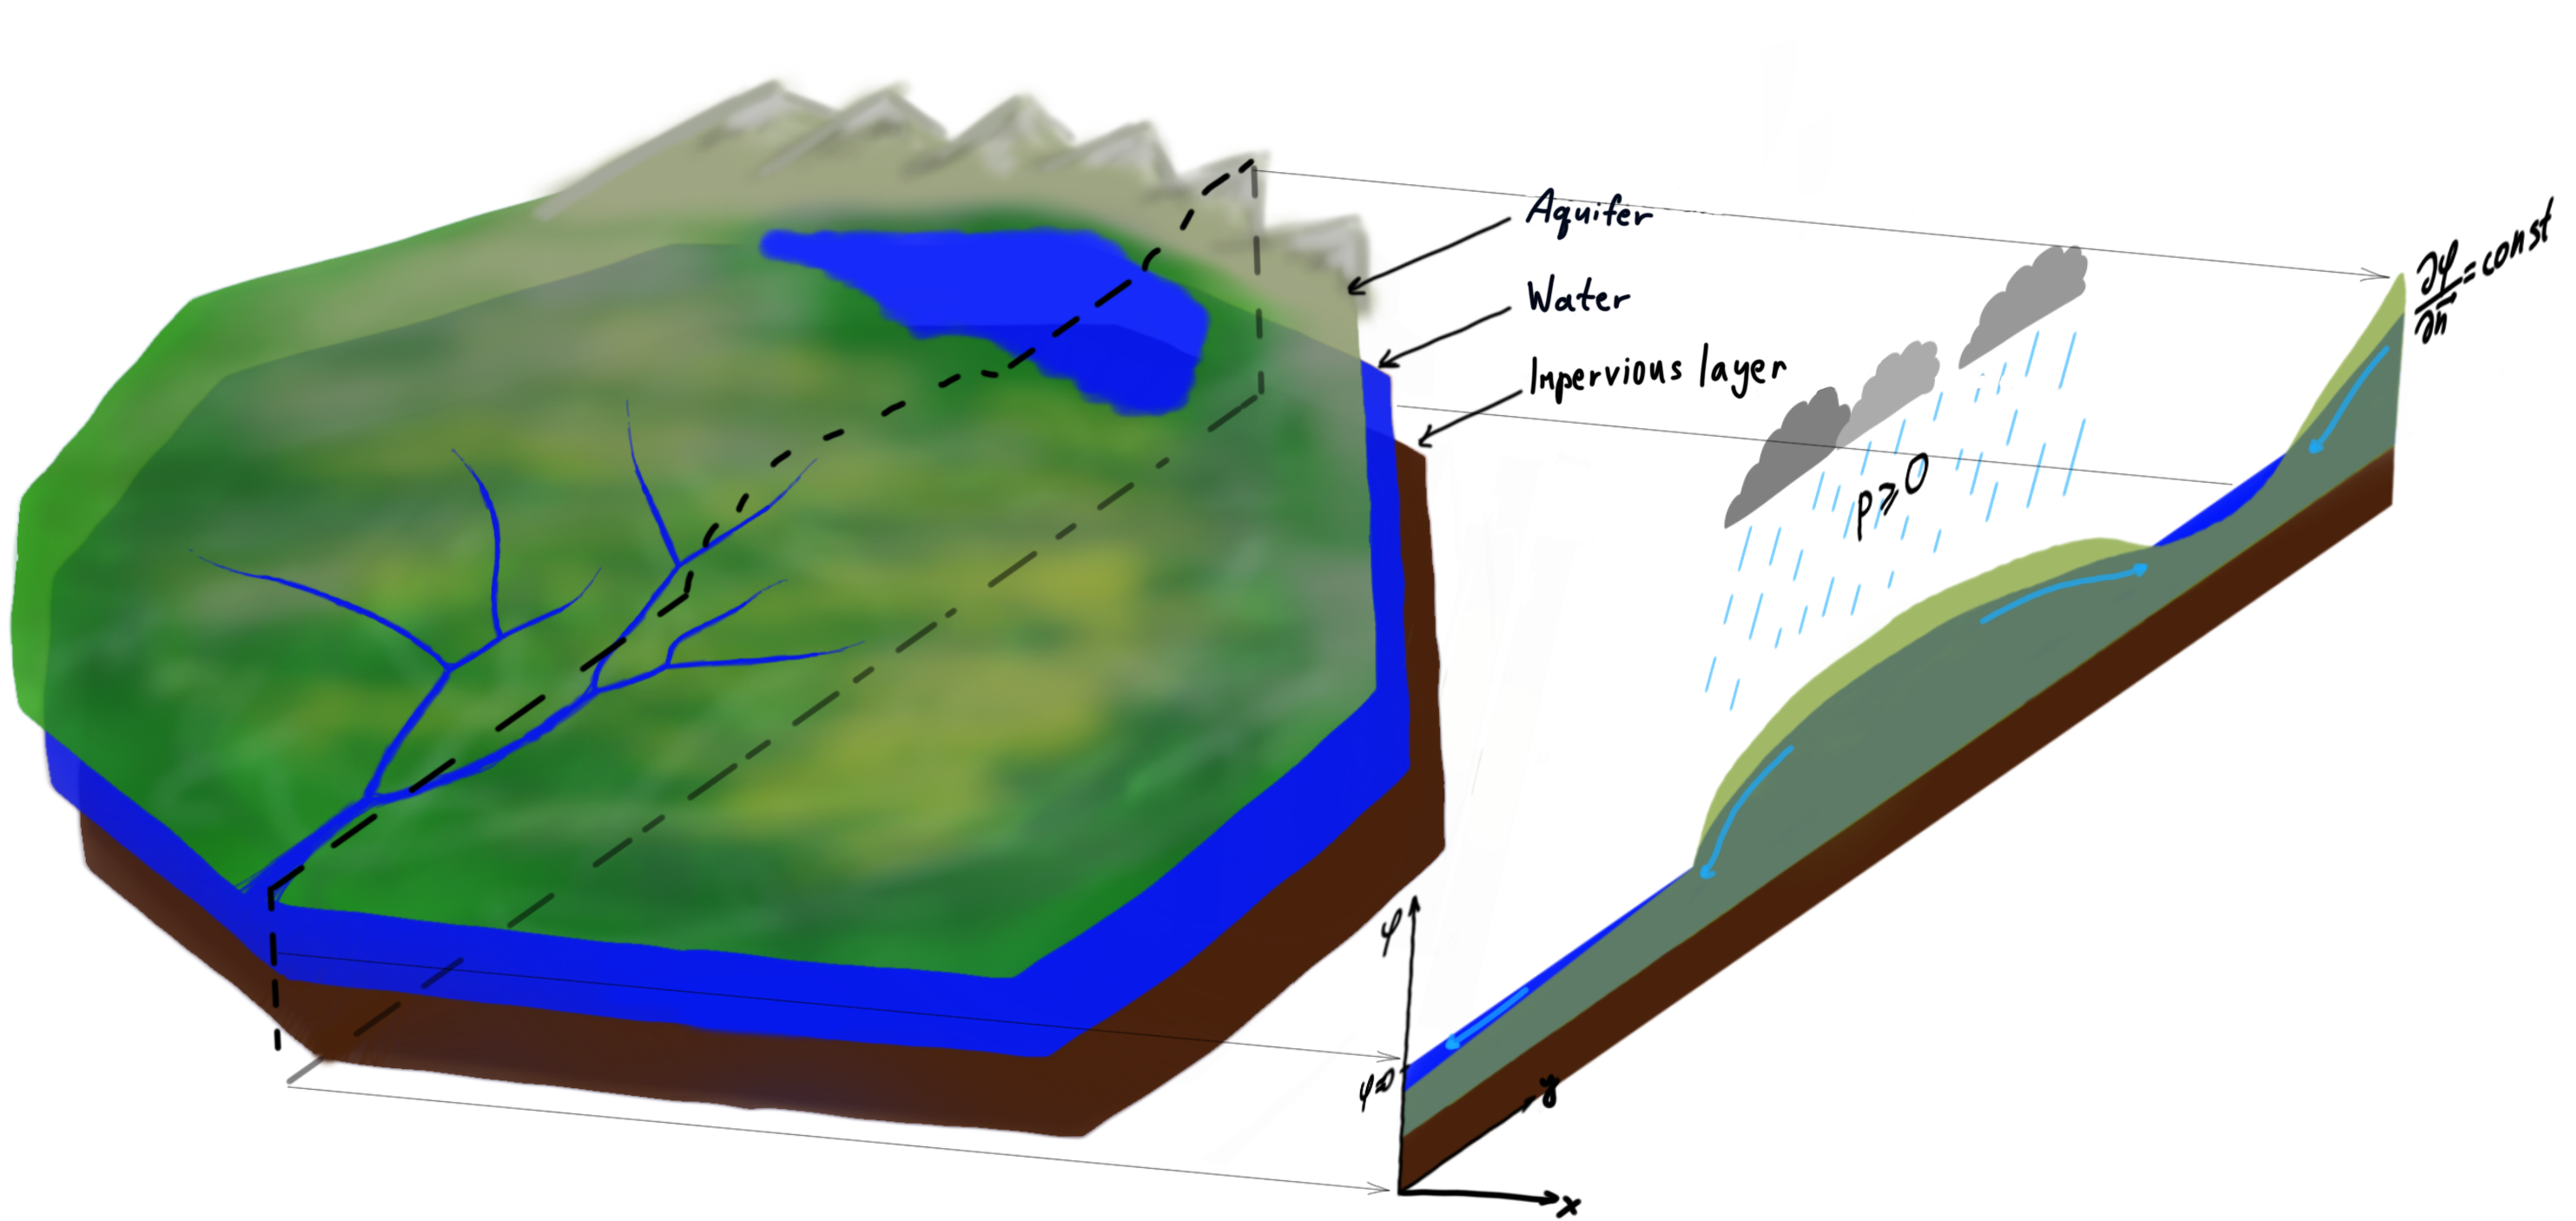
\includegraphics[width=1\textwidth]{figs/basic_river_illustration.png}
      %Dolina rzeki z jeziorem i ich przekrój. Po prawej stronie można widać jak wody podziemne są napędzane przez opady lub naprzykład przez spływ z gór.
      \caption{The river valley with the lake and their cross-section. On the right, you can see how groundwater is driven by precipitation or by runoff from mountains, for example.}
      \label{pow_wsiakanie}
    \end{figure}

    %Однак, якщо ґрунт достатньо проникний, вода може занурюватися в землю, а не стікати вниз (темно-сині стрілки на рис. \ref{float_soaking}). Вода спочатку накопичується в підземній водоймі, а потім під дією гідродинамічного тиску витікає з річкового джерела. Цей процес утворює ерозію ґрунту в околиці джерела.
    %Jeśli jednak gleba jest wystarczająco przepuszczalna, woda może wsiąkać w ziemię, zamiast spływać (ryc. \ref{pow_wsiakanie}). Woda najpierw gromadzi się w podziemnym zbiorniku, a następnie wypływa ze źródła rzeki pod wpływem ciśnienia hydrodynamicznego. Proces ten powoduje erozję gleby w pobliżu źródła.
    However, if the soil is sufficiently permeable, water can soak into the ground instead of running off (Fig. \ref{pow_wsiakanie}). Water first accumulates in an underground reservoir and then flows out of the river spring under the influence of hydrodynamic pressure. This process erodes the soil near the spring (black arrows in Fig. \ref{zrodlo}).

    \begin{wrapfigure}{r}{0.5\textwidth}
      \begin{center}
        \vspace{-20pt}
        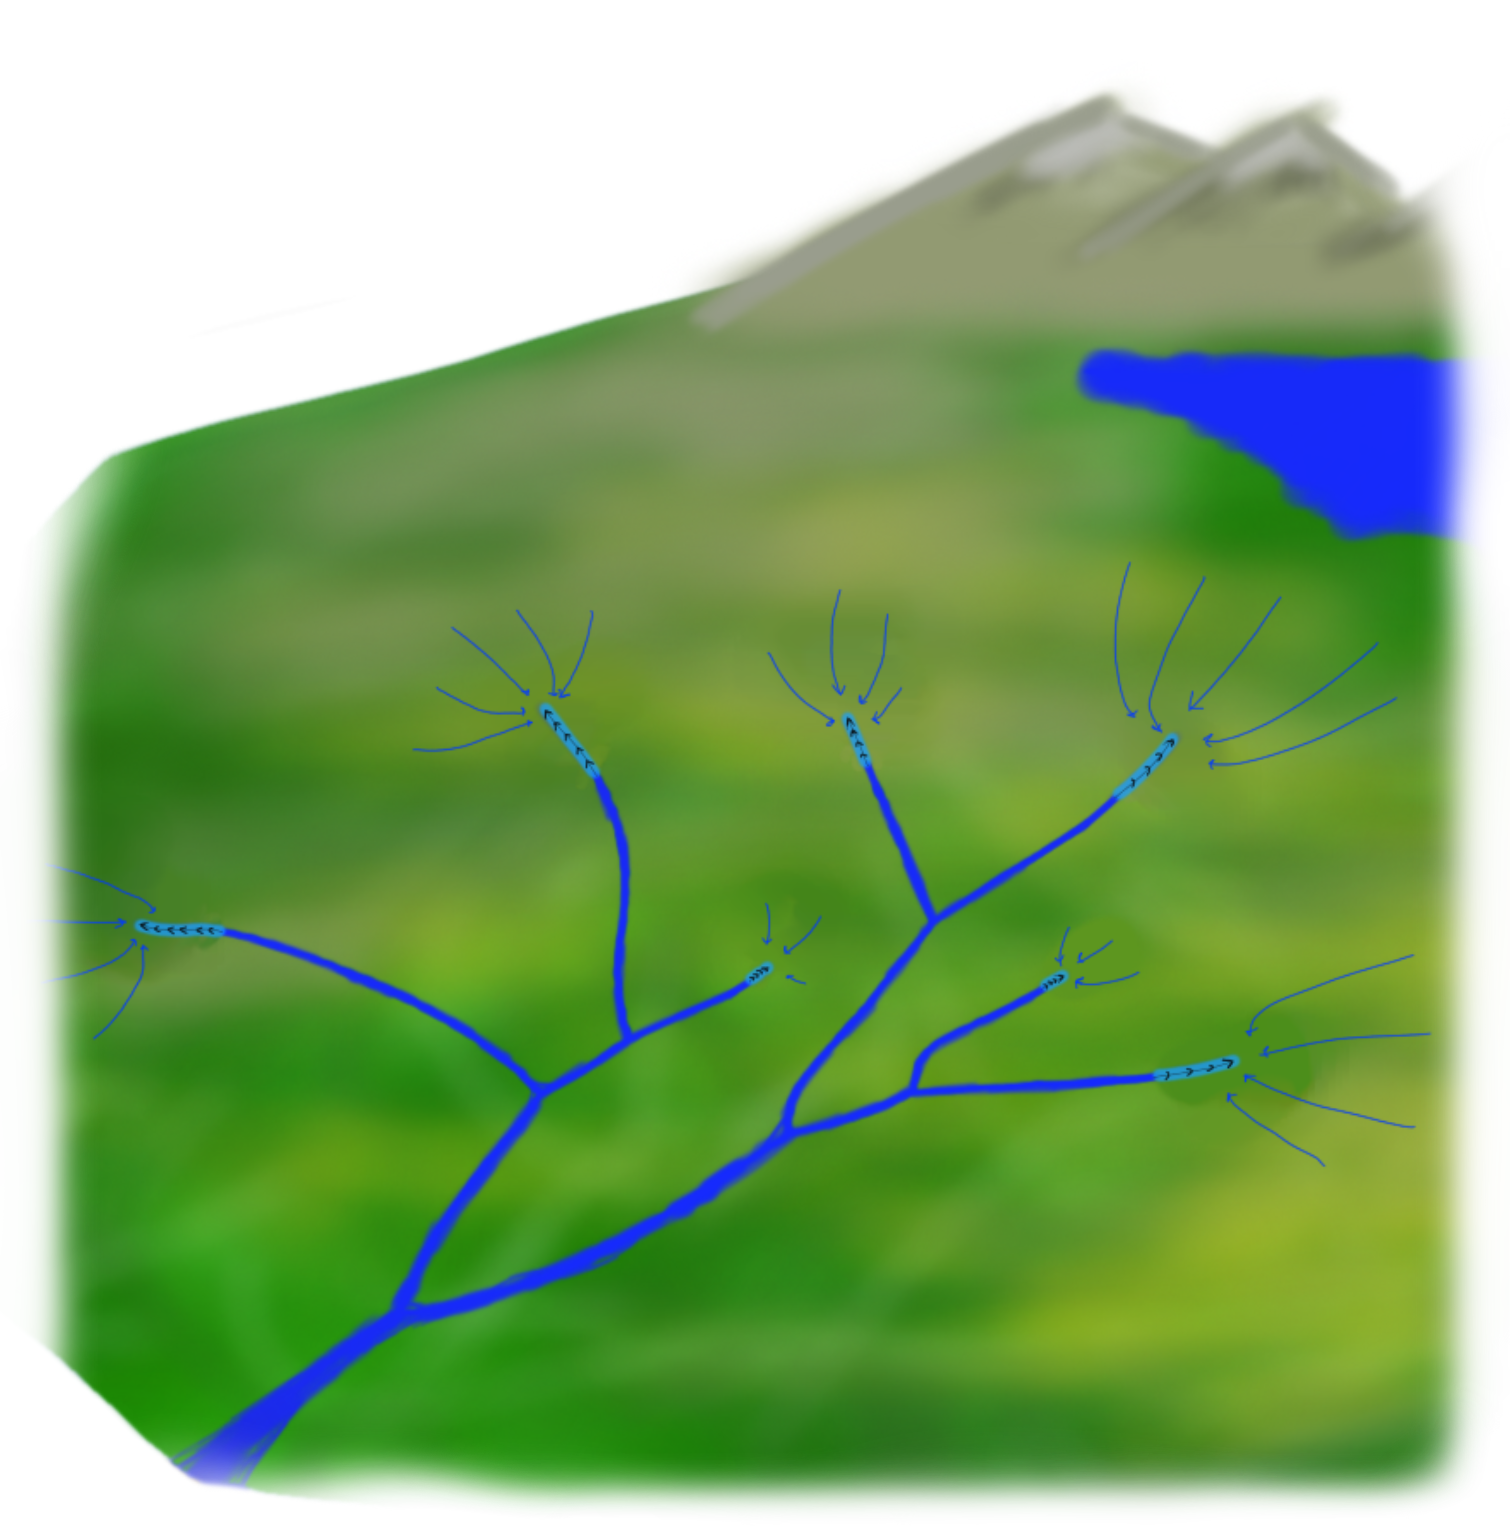
\includegraphics[width=0.45\textwidth]{figs/erosion_illustration.png}
      \end{center}
      \vspace{-20pt}
      %Ilustracja wzrostu rzeki poprzez procesy erozyjne zachodzącę w okolicy źródeł.
      \caption{Illustration of the growth of the river through erosion processes occurring in the vicinity of the springs.}
      \vspace{0pt}
      \label{zrodlo}
    \end{wrapfigure}

    %Ця ерозія в околиці джерела, котра відбувається в протилежному напрямку до течії відповідає за розширення та роздвоєння річки (біфуркація), загальну еволюцію річкової мережі.
    %Ta erozja w pobliżu źródła, która zachodzi w kierunku przeciwnym do nurtu, jest odpowiedzialna za ekspansję i bifurkację rzeki, ogólną ewolucję sieci rzecznej.
    This erosion in the vicinity of the spring, which occurs in the opposite direction to the flow, is responsible for the expansion and bifurcation of the river, the general evolution of the river network.


    %Перша кількісна модель, що описує еволюцію таких річок, була представлена ​​в 1980 році Данном \cite{dunne1980formation}. Більш детальні моделі були запропоновані групою Даніеля Ротмана з Массачусетського технологічного інституту (Refs.~\cite{petroff2012four, devauchelle2012ramification}). Автори пов’язали висоту рівня ґрунтових вод із напрямком і швидкістю зростання річки.
    %Pierwszy ilościowy model opisujący ewolucję takich rzek przedstawił w 1980 roku Dunne \cite{dunne1980formation}. Bardziej szczegółowe modele zostały zaproponowane przez grupę Daniela Rothmana z Massachusetts Institute of Technology (Refs.~\cite{petroff2012four, devauchelle2012ramification}). Autorzy powiązali wysokość poziomu wód gruntowych z kierunkiem i szybkością wzrostu rzeki.
    The first quantitative model describing the evolution of such rivers was presented in 1980 by Dunne \cite{dunne1980formation}. More detailed models have been proposed by Daniel Rothman group at the Massachusetts Institute of Technology (Refs.~\cite{petroff2012four, devauchelle2012ramification}). The authors linked the height of the groundwater table with the direction and speed of the river growth.

    %Остання модель передбачає однорідність проникної здатності і сталу висоту ґрунту, ширина річки вважається достатньо малою, а тому апроксимується лінією, а процес ерозії розглядають лише в околиці джерела.
    %Ten drugi model zakłada jednorodność przepuszczalności i stałą wysokość gruntu, szerokość rzeki uważa się za wystarczająco małą i dlatego jest przybliżona linią \cite{peterson1998singular,carleson2002laplacian,gubiec2008fingered}, a proces erozji uwzględnia się tylko w pobliżu źródła.
    The last model assumes homogeneity of permeability, the width of the river is considered small enough, and therefore is approximated by a line \cite{peterson1998singular,carleson2002laplacian,gubiec2008fingered}, and the erosion process is considered only in the vicinity of the spring.

    \section{Groundwater dynamics}

      %Wodę zgromadzoną w zbiorniku wód podziemnych opisuje prawo Darcy'ego \cite{darcy1856fontaines}:
      The movement of groundwater is described by Darcy's law \cite{darcy1856fontaines}:
      
      \begin{equation}
        \vec{u}=-\frac{\kappa}{\mu} \nabla p
      \end{equation}	
      
      %Równanie to opisuje prędkość filtracji ($\vec{u}$) płynu o lepkości dynamicznej $\mu$ przez ośrodek porowaty (np. piasek lub skały) o przepuszczalności $\kappa$ pod ciśnieniem $p$. 
      This equation describes the filtration velocity ($\vec{u}$) of a fluid with a dynamic viscosity $\mu$ through a porous medium (e.g. sand or rock) with a permeability $\kappa$ under a pressure $p$.
    
      %Aby obliczyć, ile wody przepływa przez określony punkt na płaszczyźnie $xy$, gdzie sieć się rozrasta, po prostu całkujemy prędkość Darcy'ego w danych współrzędnych $xy$ wzdłuż osi poziomej $z$ (wysokość zbiornika):
      To calculate how much water flows through a particular point in the $xy$ plane where the network grows, we simply integrate Darcy velocity in the given $xy$ coordinates along the $z$ horizontal axis (height of the groundwater table):
      
      \begin{equation}
        \vec{q}(x,y)=\int \vec{u}(x,y,z)\textrm{d}z
      \end{equation}
    
      %Teraz korzystamy z założenia Dupuit \cite{dupuit1863etudes}, które mówi, że wody gruntowe płyną poziomo. Ponadto zakładamy, że ciśnienie powodujące przepływ jest po prostu ciśnieniem hydrostatycznym $p = \rho g h $ ($\rho$ -- gęstość wody, $g$ -- przyspieszenie grawitacyjne, $h$ -- wysokość Tabela wód podziemnych). Dla takiego ciśnienia $\nabla p$ jest niezależne od współrzędnej $z$, a powyższa całka upraszcza się do iloczynu prędkości filtracji $\vec{u}$ i wysokości słupa wody $h(x, y)$ w danym miejscu:
      Now we use the Dupuit \cite{dupuit1863etudes} assumption that groundwater flows horizontally. In addition, we assume that the pressure causing the flow is simply hydrostatic pressure $p = \rho g h $ ($\rho$ -- density of water, $g$ -- gravitational acceleration, $h$ -- height of groundwater table). For such a pressure, $\nabla p$ is independent of the $z$ coordinate, and the above integral simplifies to the product of the filtration velocity $\vec{u}$ and the height of the water column $h(x, y)$ at a given location:
      
      \begin{equation}
        \label{qq}
        \vec{q}(x,y)=h\vec{u}=-h \frac{\kappa}{\mu} \nabla(\rho g h)=-\nabla \left(\frac{\kappa \rho g}{2\mu}h^2(x,y)\right) = - \nabla \phi(x,y) \,,
      \end{equation}
      
      %gdzie wprowadziliśmy potencjał $\phi(x,y)$:
      where we defined the groundwater potential $\phi(x,y)$:
      
      \begin{equation}
        \phi(x,y) = \frac{\kappa \rho g}{2\mu}h^2(x,y) \,.
      \end{equation}
    
      %Na koniec wyprowadzamy równania opisujące pole $\phi$ z równania ciągłości, uwzględniając opady (opisane przez średnią objętość opadów na jednostkę czasu i powierzchnię — $P$). Zmianę masy kolumny płynu ($M$) zamkniętej w obszarze $S$ można opisać następująco:
      Now we can derive the equation describing the field $\phi$ from the continuity equation, taking into account rainfall (described by the average volume of precipitation per unit time and area, $P$). The mass change of the fluid column ($M$) enclosed in the $S$ area can be described as follows:
      

      \begin{gather*}
        \frac{\partial M}{\partial t}=- \int\limits_{\partial S} \vec{q}\cdot \hat{n} \ \textrm{d}l + \int\limits_S P \ \textrm{d}S
        \\
        \frac{\partial}{\partial t} \int\limits_S \rho h \ \textrm{d}S=\int\limits_S \left(-\nabla \cdot \vec{q} + P\right)\textrm{d}S
        \\
        \rho \frac{\partial h}{\partial t}=-\nabla \cdot \vec{q} + P
      \end{gather*}	

      %W tym miejscu należy skomentować skale czasowe w rzeczywistych systemach. Średni czas między opadami to 10 dni, a średni czas przepływu wody przez system to $10^4$ dni. Oznacza to, że wahania wysokości zwierciadła wód gruntowych $h$ są bardzo małe i jako $P$ możemy przyjąć średnią roczną wielkość opadów. Ponadto szybkość wzrostu sieci rzecznej szacuje się na około 1~mm/rok, a charakterystyczny czas zmian geometrii to $10^4$ lat. To z kolei oznacza, że w skalach czasowych odpowiadających wzrostowi sieci rzecznej możemy pominąć $ \frac{\partial h} {\partial t} $ w równaniu ciągłości, otrzymując:
      Time scales in real systems should be commented on here. The average time between precipitation is 10 days, and the average time for water to flow through the system is $10^4$ days. This means that fluctuations in the height of the groundwater table $h$ are very small and as $P$ we can assume the average annual amount of precipitation. In addition, the growth rate of the river network is estimated at about 1~mm/year, and the characteristic time of geometry changes is $10^4$ years. This in turn means that on time scales corresponding to the growth of the river network, we can omit $ \frac{\partial h} {\partial t} $ in the continuity equation, yielding:  
      
      \begin{equation}
    		\nabla \cdot \vec{q} = P \,.
    	\end{equation}
      
      %Używając wcześniej zdefiniowanego potencjału $\phi$ otrzymujemy równanie Poissona:
      Using the previously defined potential $\phi$ we get the Poisson equation:
      
      \begin{equation}
        \label{poisson}
    		\Delta \phi = -P/\kappa
    	\end{equation}
      
      %lub równanie Laplace'a, gdzie nie ma opadów ($P=0$):
      or the Laplace equation where there is no precipitation ($P=0$)
      
      \begin{equation}
        \label{laplace}
    		\Delta \phi = 0 \,.
    	\end{equation}	

      %Równania te muszą być uzupełnione odpowiednimi warunkami brzegowymi. W naszym przypadku zakładamy, że rzeka płynie bezpośrednio po warstwie nieprzepuszczalnej (przy $h = 0$), czyli $\phi = 0$ na całej jej długości. Dodatkowo granice domeny są często nieprzepuszczalne, co można zapisać jako odblaskowy warunek brzegowy ($\frac{\partial \phi}{\partial \vec{n}} = 0$). Wreszcie, gdy nie ma opadów, zakładamy, że woda wchodzi do układu przez jedną z granic (na przykład z odległych lodowców) -- można to opisać jako stały przepływ pola $\phi$ wzdłuż rozważanej ściany ($\frac{\partial \phi}{\partial \vec{n}} = const.$).
      These equations must be supplemented with appropriate boundary conditions. In our case, we assume that the river flows directly over the impermeable layer (with $h = 0$), i.e. $\phi = 0$ along its entire length. Additionally, domain boundaries are often impermeable, which can be written as a reflective boundary condition ($\frac{\partial \phi}{\partial \vec{n}} = 0$). Finally, when there is no precipitation, we assume that water enters the system through one of the boundaries (for example, from distant glaciers) -- this can be described as a constant flow of the $\phi$ field along the wall under consideration ($\frac{\partial \phi }{\partial \vec{n}} = const.$).
      
      %W ten sposób udało nam się zredukować trójwymiarowy problem przepływu płynów do obliczenia dwuwymiarowego potencjału, który niesie pełną informację o dynamice wód gruntowych.
      In this way, we were able to reduce the three-dimensional problem of fluid flow to the calculation of a two-dimensional potential, which carries full information about groundwater dynamics.

  \section{Solving Laplace's equation}\label{chapter:solving}
    
    %We współrzędnych biegunowych (gdzie kierunek stycznej do palca na wierzchołku ustawia $\theta = 0$) pole w pobliżu wierzchołka można rozszerzyć \cite{derrida1992needle , petroff2013bifurcation}:
    In polar coordinates (where the direction of the tangent to the finger at the tip sets $\theta = 0$), the field near the spring can be extended \cite{derrida1992needle , petroff2013bifurcation}:
    
    \begin{equation}\label{phi_polar}
      \phi(r,\theta)=a_1r^{1/2}\cos\frac{\theta}{2}+a_2r \sin \theta+a_3 r^{3/2} \cos\frac{3\theta}{2}+\mathcal{O}\left(r^2\right) \,,
    \end{equation}

    %Równ. \eqref{phi_polar} obowiązuje również w przypadku pól Poissona, ponieważ w sąsiedztwie wierzchołka wkład strumienia z członu źródłowego jest pomijalny w porównaniu do strumienia z obszarów oddalonych od wierzchołka. Dla każdego z wiodących współczynników $a_i$ w równaniu \eqref{phi_polar} możemy znaleźć interpretację fizyczną.
    Eq. \eqref{phi_polar} is also valid for Poisson fields, because in the vicinity of the tip point the contribution of the flux from the source term is negligible compared to the flux from areas far from the spring. For each of the leading coefficients $a_i$ in the equation \eqref{phi_polar} we can find a physical interpretation.

    %Po pierwsze, współczynnik $a_1$ jest powiązany z całkowitym strumieniem na małym okręgu o promieniu $r_0$ wokół końcówki:
    First, the coefficient $a_1$ is related to the total flux in a small circle of radius $r_0$ around the tip: 
    
    \begin{equation}\label{circle}
      J|_{r_0} = \oint_{r_0} (-\kappa \nabla \phi) \cdot \hat{n} \ \textrm{d}l = 2 \kappa a_1 r_0^{1/2} + \mathcal{O}\left(r_0^{3/2}\right) \,.
    \end{equation}

    %Współczynnik $a_2$ jest powiązany z asymetrią pola wokół wierzchołka. Przy dodatnim $a_2$ strumień pola jest większy po prawej stronie wierzchołka, a przy ujemnym $a_2$ — po lewej stronie. Palec rośnie jednak w kierunku największego strumienia i w efekcie rośnie w taki sposób, że $a_2$ zawsze znika (zasada lokalnej symetrii \cite{cohen2015path}).
    The $a_2$ coefficient is related to the asymmetry of the field around the tip. With positive $a_2$, the field flux is greater on the right side of the tip, and with negative $a_2$ - on the left side. However, the finger grows in the direction of the greatest flux, and in effect grows in such a way that $a_2$ always vanishes (the principle of local symmetry \cite{cohen2015path}).
    
    %Wreszcie $a_3$ jest połączona z drugą pochodną pola. Jeśli ponownie skupimy się na małym okręgu o promieniu $r_0$ wokół końcówki i zbadamy pole jako funkcję kąta $\theta$, zauważymy, że przy ustalonych $a_1>0$ i $a_2=a_3=0$ pole ma pojedyncze maksimum przy $\theta = 0$. Im mniejszy współczynnik $a_3$, tym bardziej płaskie maksimum pola wokół końcówki. W końcu, gdy druga pochodna $\phi$ znika, co odpowiada ujemnej wartości $a_3/a_1$:
    Finally, $a_3$ is related to the second derivative of the field. If we focus again on the small circle of radius $r_0$ around the tip and examine the field as a function of the angle $\theta$, we see that given $a_1>0$ and $a_2=a_3=0$ the field has a single maximum at $\theta = $0. The smaller the $a_3$ factor, the flatter the field maximum around the tip. Finally, when the second derivative of $\phi$ disappears:
    
    \begin{equation}\label{a3a1}
      \frac{\partial^2 \phi}{\partial \theta^2}\big|_{\theta=0, r=r_0} = 0 \implies a_3/a_1 = -\frac{1}{9 r_0} \,, 
    \end{equation}
    
    %to pojedyncze maksimum przekształca się w dwa maksima w $\pm \theta_0$. Zauważ, że wartość progowa $a_3/a_1$ zależy od odległości $r_0$ od końcówki, przy której analizowane jest pole. Dla nieskończenie małych $r_0$ profil pola jest zawsze symetryczny z jednym maksimum przy $\theta=0$.
    This single maximum splits into two maxima at $\pm \theta_0$. Note that the threshold value $a_3/a_1$ depends on the distance $r_0$ from the tip where the field is analyzed. For infinitesimal $r_0$ the profile of the field is always symmetric with one maximum at $\theta=0$.

    %Aby otrzymać współczynniki $a_i$, możemy po prostu rozwiązać odpowiednie równanie dla pola (Laplace'a lub Poissona) metodą elementów skończonych, a następnie korzystając z postaci całkowej współczynników:
    To get the coefficients $a_i$, the appropriate equation for the field (Laplace or Poisson) should be solved using the finite element method and then using the integral form of the coefficients:
    
    \begin{equation}
      \label{a1}
      a_1 = \frac{1}{\pi r_0^{1/2}}\int^{\pi}_{-\pi} \phi(r_0,\theta)\cos\frac{\theta}{2}\textrm{d}\theta \,,
    \end{equation} 
    
    \begin{equation}
      \label{a2}
      a_2 = \frac{1}{\pi r_0}\int^{\pi}_{-\pi} \phi(r_0,\theta)\sin\theta \textrm{d}\theta \,,
    \end{equation}
    
    \begin{equation}
      \label{a3}
      a_3 = \frac{1}{\pi r_0^{3/2}}\int^{\pi}_{-\pi} \phi(r_0,\theta)\cos\frac{3\theta}{2}\textrm{d}\theta
    \end{equation}	
    
    %obliczyć je. Przeprowadzamy ją w programie Riversim który był inspirowany rozwiązaniem w FreeFEM++\cite{hecht2012new} początkowo stworzonych przez grupę Daniela Rothmana w MIT \cite{petroff2011geometry, petroff2013bifurcation, cohen2015path} i dalej rozwijanych w grupie Piotra Szymczaka \cite{morawiecki2016problem, zukowski2019zwiazek}.



  \section{Evolution of the river network}
    
    %\subsection{Reguły wzrostu}

    %W najogólniejszym przypadku prędkość wzrostu może być dowolną funkcją pola ($v = f(\phi)$), ale w klasycznym wzroście Laplace'a jest proporcjonalna do gradientu pola -- $f(\phi) = \alpha |\nabla \phi|$, gdzie $\alpha$ jest stałą proporcjonalności. Jednak, prawo potęgowe zostały odnotowane w wielu różnych systemach fizycznych, np. przebicie dielektryczne \cite{niemeyer1984fractal} i -- po tych pracach -- założymy tutaj, że prędkość końcówki jest proporcjonalna do strumienia wchodzącego w nią pola ($J$) do potęgi $\eta$. Przypominając równanie \eqref{circle} mamy \cite{carleson2002laplacian, selander1999two}:
    In the most general case, the growth rate can be any function of the field ($v = f(\phi)$), but in classical Laplace growth it is proportional to the gradient of the field -- $f(\phi) = \alpha |\nabla \phi |$, where $\alpha$ is a constant of proportionality. However, power law has been reported in many different physical systems, e.g. dielectric breakdown \cite{niemeyer1984fractal} and - following this work - we will assume here that the speed of the tip is proportional to the flux of the field entering it ($J$) to the power $\eta$. Recalling the equation \eqref{circle} we have \cite{carleson2002laplacian, selander1999two}:
       
    \begin{equation}\label{velocity}
      v = \alpha a_1^\eta \,.
    \end{equation}
      
    %W literaturze dotyczącej modelu cienkiego palca stosuje się dwa różne deterministyczne kryteria podziału -- kryterium prędkości i kryterium kształtu pola. Pierwsze kryterium może być wprost zaimplementowane w modelu cienkiego palca jako próg $a_1$: $a_1 > a_1^c$.
    In the literature on the thin finger model two different deterministic division criteria are used - the velocity criterion and the field shape criterion. The first criterion can be directly implemented in the thin finger model as the $a_1$ threshold: $a_1 > a_1^c$.

    %Drugie kryterium jest związane z ekstremami strumienia (w funkcji kąta biegunowego) \cite{petroff2013bifurcation, kaandorp2001algorithmic_Chapter4.4}, a więc ze współczynnikiem $a_3$. Gdy dla danego promienia $r_0$ strumień pola ma wysokie pojedyncze maksimum, palec rośnie w kierunku tego maksimum. Jeśli jednak strumień pola z boków wierzchołka staje się porównywalny do tego z przodu, a nawet w końcu staje się większy (co odpowiada pojawieniu się dwóch maksimów przy $\pm \theta_0$), palec próbuje rosnąć w dwóch kierunkach jednocześnie, co skutkuje bifurkacją. Mówiąc dokładniej, mówimy, że palec dzieli się, gdy $a_3/a_1$ jest mniejsze niż jakaś wartość krytyczna.
    The second criterion is related to the extremes of the flux (as a function of the polar angle) \cite{petroff2013bifurcation, kaandorp2001algorithmic_Chapter4.4}, i.e. with the coefficient $a_3$. When, for a given radius $r_0$, the field flux has a high single maximum, the finger grows towards this maximum. However, if the field flux from the sides of the spring becomes comparable to that of the front, and even eventually becomes larger (corresponding to the appearance of two maxima at $\pm \theta_0$), the finger tries to grow in two directions at once, resulting in a bifurcation. More precisely, we say that the finger splits when $a_3/a_1$ is less than some critical value.

  \chapter{Numerical solution and software structure}

    %\hspace{1em} \= 
    %Pole wód podziemnych kształtuję erozje w oklicy żródła i jak skutek dynamikę i rozwój sięci. Z matematycznego modelu dla opisu sieci rzecznych otrzymujemy równania dla opisu wód podziemnych w postaci równania Laplacea \ref{laplace}(lub Poissona \ref{poisson}). Pole w okolicy źródła jest aproxymowane współcznynnikami $a_i$ (\ref{a1} \ref{a2} \ref{a3}). Całkowanie współcznynników jak i rozwiązywanie też w swoją kolej wymaga metod numerycznych. W ogólnym przypadku równanie Laplace można rozwiązać metodami numerycznymi, a w szczegolności w tej pracy skorzystano z metody skończonych elementów. \\ \indent
    \hspace{1em} 
    The groundwater field is shaped by erosion in the vicinity of the spring and, as a result, the dynamics and development of the network. From the mathematical model for the description of river networks, we obtain equations for the description of groundwater in the form of the Laplace \ref{laplace} (or Poisson \ref{poisson}) equation. The field near the spring is approximated by the coefficients $a_i$ (\ref{a1} \ref{a2} \ref{a3}). Evaluation of the coefficients $a_i$ as well as solving groundwater field $\phi(x, y)$ requires numerical methods. In general, the Laplacian equation can be solved by numerical methods, and in particular, the finite element method was used in this work. \\ \indent
    
    %В попередніх проектах вже було представлені рішення для задачі еволюції мережі річки. Один з розв'язків був написаний з використанням Фреефем++ і Матлаб. Інший, з допомогою конформних перетворень. Однак для отримання і ще більших мереж річок потрібен був оптимальніший розв'язок. Другою вимогою було використання тільки технологій із відкритим вихідним кодом, адже не кожен має можливість придбати Матлаб. Вибір припав на C++\cite{Stroustrup1997} та Python. Адже ці мови програмування є одними з найбілш росповсюдженних, а також містять в собі багато бібліотек із відкритим кодом, що полегшує написання програм. C++ -- з одного боку, він дуже швидкий, але вимогливий до написання. С++ містить реалізацію частини програми, яка займає є складною в обчисленнях, такі як алгоритми для роботи із геометрією, генерацією сітки, розязок диференціальних рівняннь. Python\cite{python3} -- має меншу обчислювальну ефективність, але набагато швидший у розробці програмного забезпечення і надає інтерактивний інструмент для написання скрипту -- Jupyter.  
    %W poprzednich projektach prezentowano już rozwiązania problemu ewolucji sieci rzecznej. Jedno z rozwiązań zostało napisane przy użyciu Freefem++ i Matlaba. Inny, za pomocą przekształceń konforemnych. Jednak aby uzyskać jeszcze większe sieci rzeczne, potrzebne było bardziej optymalne rozwiązanie. Drugim wymogiem było korzystanie wyłącznie z technologii z otwartym kodem źródłowym, ponieważ nie każdy ma możliwość zakupu Matlaba. Wybór padł na C++\cite{Stroustrup1997} i Python\cite{python3}. W końcu te języki programowania należą do najbardziej rozpowszechnionych, a także zawierają wiele bibliotek z otwartym źródłołem kodem, co ułatwia pisanie programów. C++ -- z jednej strony jest bardzo szybki, ale wymagający w pisaniu. C++ zawiera implementację części programu, która jest złożona w obliczeniach, takich jak algorytmy pracy z geometrią, generowanie siatki i rozwiązywanie równań różniczkowych. Python — ma mniejszą wydajność obliczeniową, ale jest znacznie szybszy w tworzeniu oprogramowania i zapewnia interaktywne narzędzie do tworzenia skryptów — Jupyter.
    In previous projects, solutions for the problem of the evolution of the river network have already been presented. One of the solutions was written using Freefem++ and Matlab. Another, with the help of conformal transformations. However, in order to obtain even larger river networks, a more optimal solution was needed. The second requirement was to use only technologies with open source code, because not everyone has the opportunity to purchase Matlab. The choice fell on C++\cite{Stroustrup1997} and Python. After all, these programming languages are among the most widespread, and also contain many open source libraries, which makes it easier to write programs. C++ -- it is very fast, but demanding to write. Python\cite{python3} -- is less computationally efficient, but much faster in software development and provides an interactive scripting tool -- Jupyter.

    \begin{figure}[H]
      \centering
      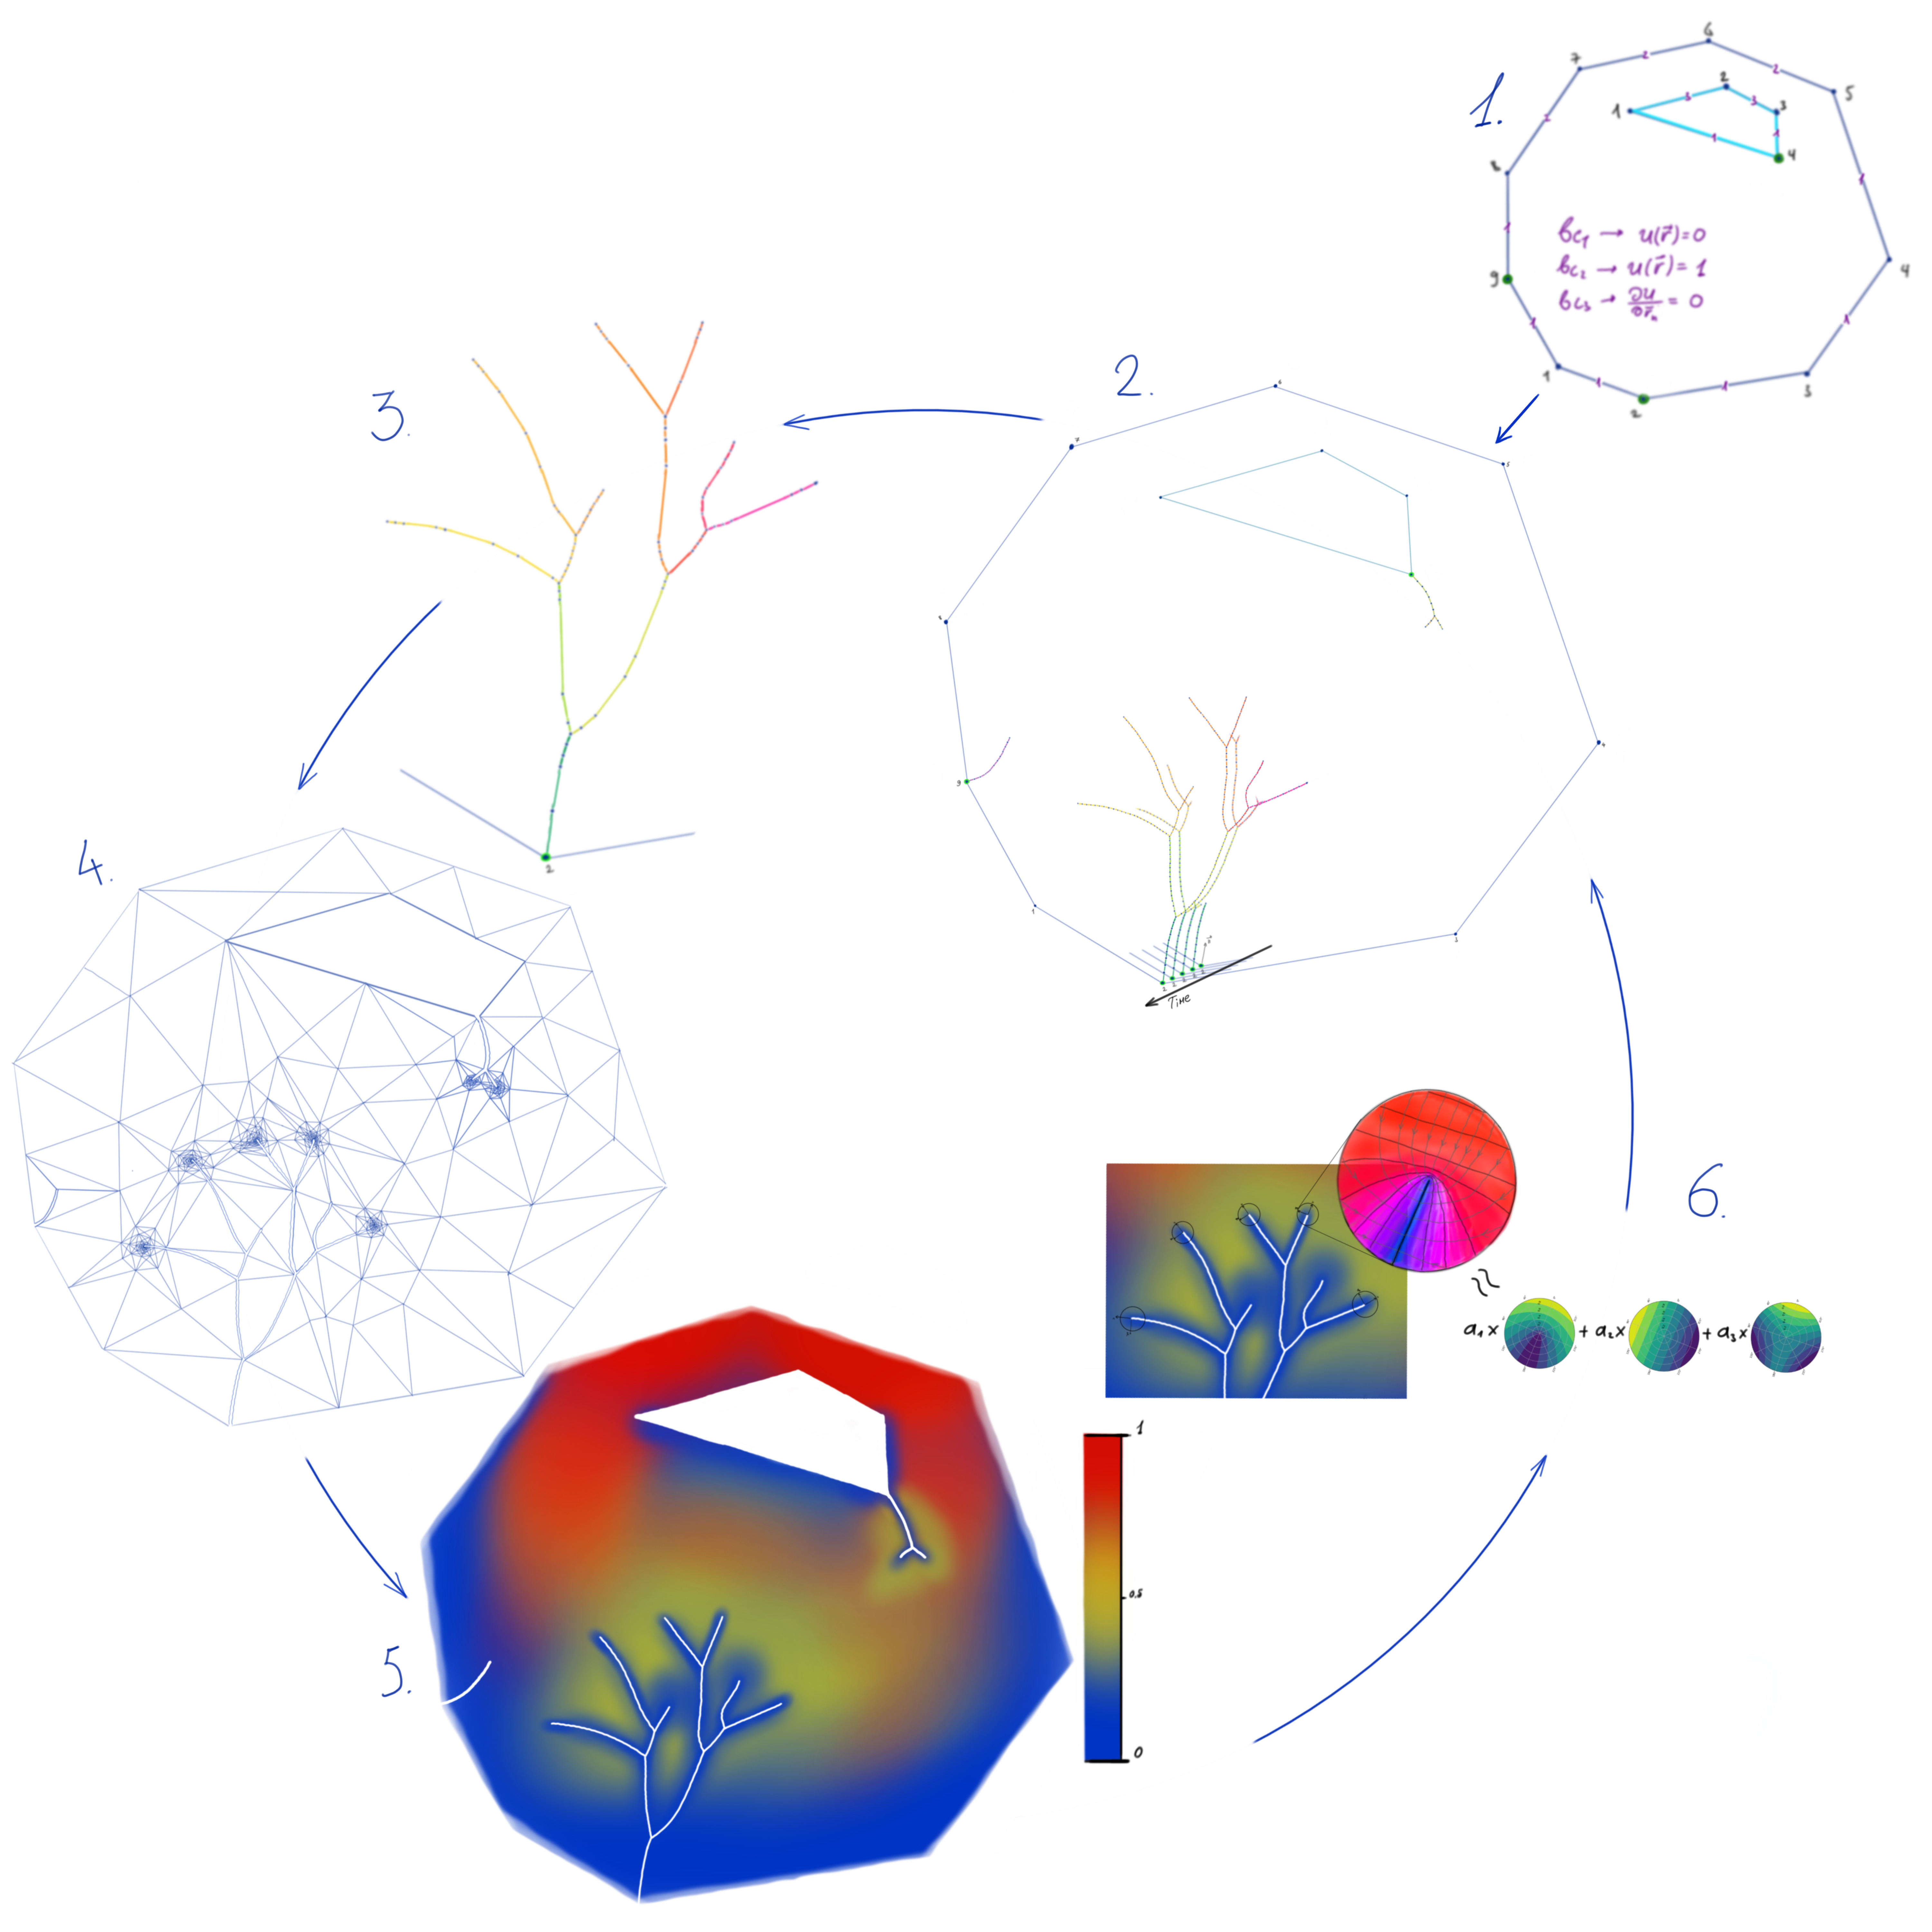
\includegraphics[width=1\textwidth]{figs/ProgramWorkflowMainIllustration.png}
      %(1) Початкова геометрія, задавання місць на границі звідки буде рости річка, граничні умови. (2) Початкова мережа річки(можна не задавати). (3) Спрощення геометрії річки. (4) Генерація дрібнозернистого мешу. (5) Розв'язок диференційних рівнянь. (6) Визначення параметрів ряду довкола джерел. (2) Ріст мережі річки.
      %Метод конечних елементів вимагає визначення геометрії області, потім її дискретизація, створення лінійних рівнянь, розв’язування рівнянь, інтегрування коефіцієнти $a_i$ розкладу в ряд. Наведені вище кроки формують структуру програмного забезпечення \ref{program_workflow}.
      %Metoda elementów skończonych wymaga wyznaczenia geometrii obszaru, następnie jej dyskretyzacji, utworzenia równań liniowych, rozwiązania równań, zintegrowania współczynników rozszerzenia $a_i$ w szereg. Powyższe kroki tworzą strukturę oprogramowania. (1) Geometria początkowa, ustalenie miejsc na granicy, z których rzeka będzie wypływać i warunki brzegowe. (2) Początkowa sieć rzeki (opcjonalnie). (3) Uproszczenie geometrii rzeki. (4) Generowanie drobnoziarnistej siatki. (5) Rozwiązywanie równań różniczkowych. (6) Wyznaczanie parametrów szeregu wokół źródeł. (2) Wzrost sieci rzecznej.
      \caption{The finite element method requires determining the geometry of the area, then discretizing it, creating linear equations, solving the equations, integrating the expansion factors $a_i$ into a series. The above steps form the structure of the software. (1) Initial geometry, determination of boundary locations from which the river will flow, and boundary conditions. (2) Initial river network (optional). (3) Simplifying the geometry of the river. (4) Fine mesh generation. (5) Solving differential equations. (6) Determining the parameters of the series around the springs. (2) Growth of the river network.}
      \label{program_workflow}
    \end{figure}
      
    %W trakcie tworzenia oprogramowania było stworzono dwa rzowiązania: Riversim\cite{Riversim} - program który zawiera wszystkie algorytmy dla generacji sieci rzecznych, Riversimpy\cite{Riversimpy} - biblioteka w Pythonie które zawiera algorytmy ułatwiające tworzenie skryptów dla symulacji wzrostu sieci w polu Laplasowskim. 
    During software development two solutions were created: Riversim\cite{Riversim} - a program that contains all the algorithms for river network generation, Riversimpy\cite{Riversimpy} - a Python library that contains algorithms that facilitate the creation of scripts for simulating network growth in a Laplacian field.
    
    %Riversim zawiera niektórę dodatkowe algorytmy dla odwracalnej ewolucji wsztecznej i do przodu, a poza tym Riversim i Riversimpy zawierają tę same algorytmy, w podalszym opisie głównie skupimysię na Riversimpy. 
    Riversim includes some additional algorithms for reversible backward and forward evolution, but except of this Riversim and Riversimpy contain the same algorithms and are build aroud workflow shown on Fig. \ref{program_workflow}, in the following description we will focus on Riversimpy.

    \section{Geometry}
      
      %В реальних середовищах еволюції русла річок даного типу, ми можемо зустріти цілий ряд чинників, котрі мають вплив на поле підземних вод. Наприклад, це можуть бути гори звідки регулярно надходить потік води, озеро котре може слугувати кінцевою точкою або початком річки. Мережа річки теж має вплив на поле підземних вод і багато інших чинників. Ця довільність геометрії продемонстрована на малюнку \ref{geometry_examples}.
      %W rzeczywistych środowiskach ewolucji koryt rzecznych możemy napotkać szereg czynników, które mają wpływ na pole wód gruntowych. Na przykład mogą to być góry, z których regularnie wypływa strumień wody, jezioro, które może służyć jako punkt końcowy lub początek rzeki. Sieć rzeczna ma również wpływ na pole wód gruntowych i wiele innych czynników. Ta arbitralność geometrii jest pokazana na rysunku \ref{geometry_examples}.
      In the real environments of the evolution of riverbeds of this type, we can meet a number of factors that have an impact on the groundwater field. For example, these can be mountains from which a stream of water regularly flows, a lake that can serve as the end point or the beginning of a river and the river network itself. Example of domain is demonstrated in the Fig. \ref{geometry_examples}.
      
      \begin{figure}[H]
        \centering
        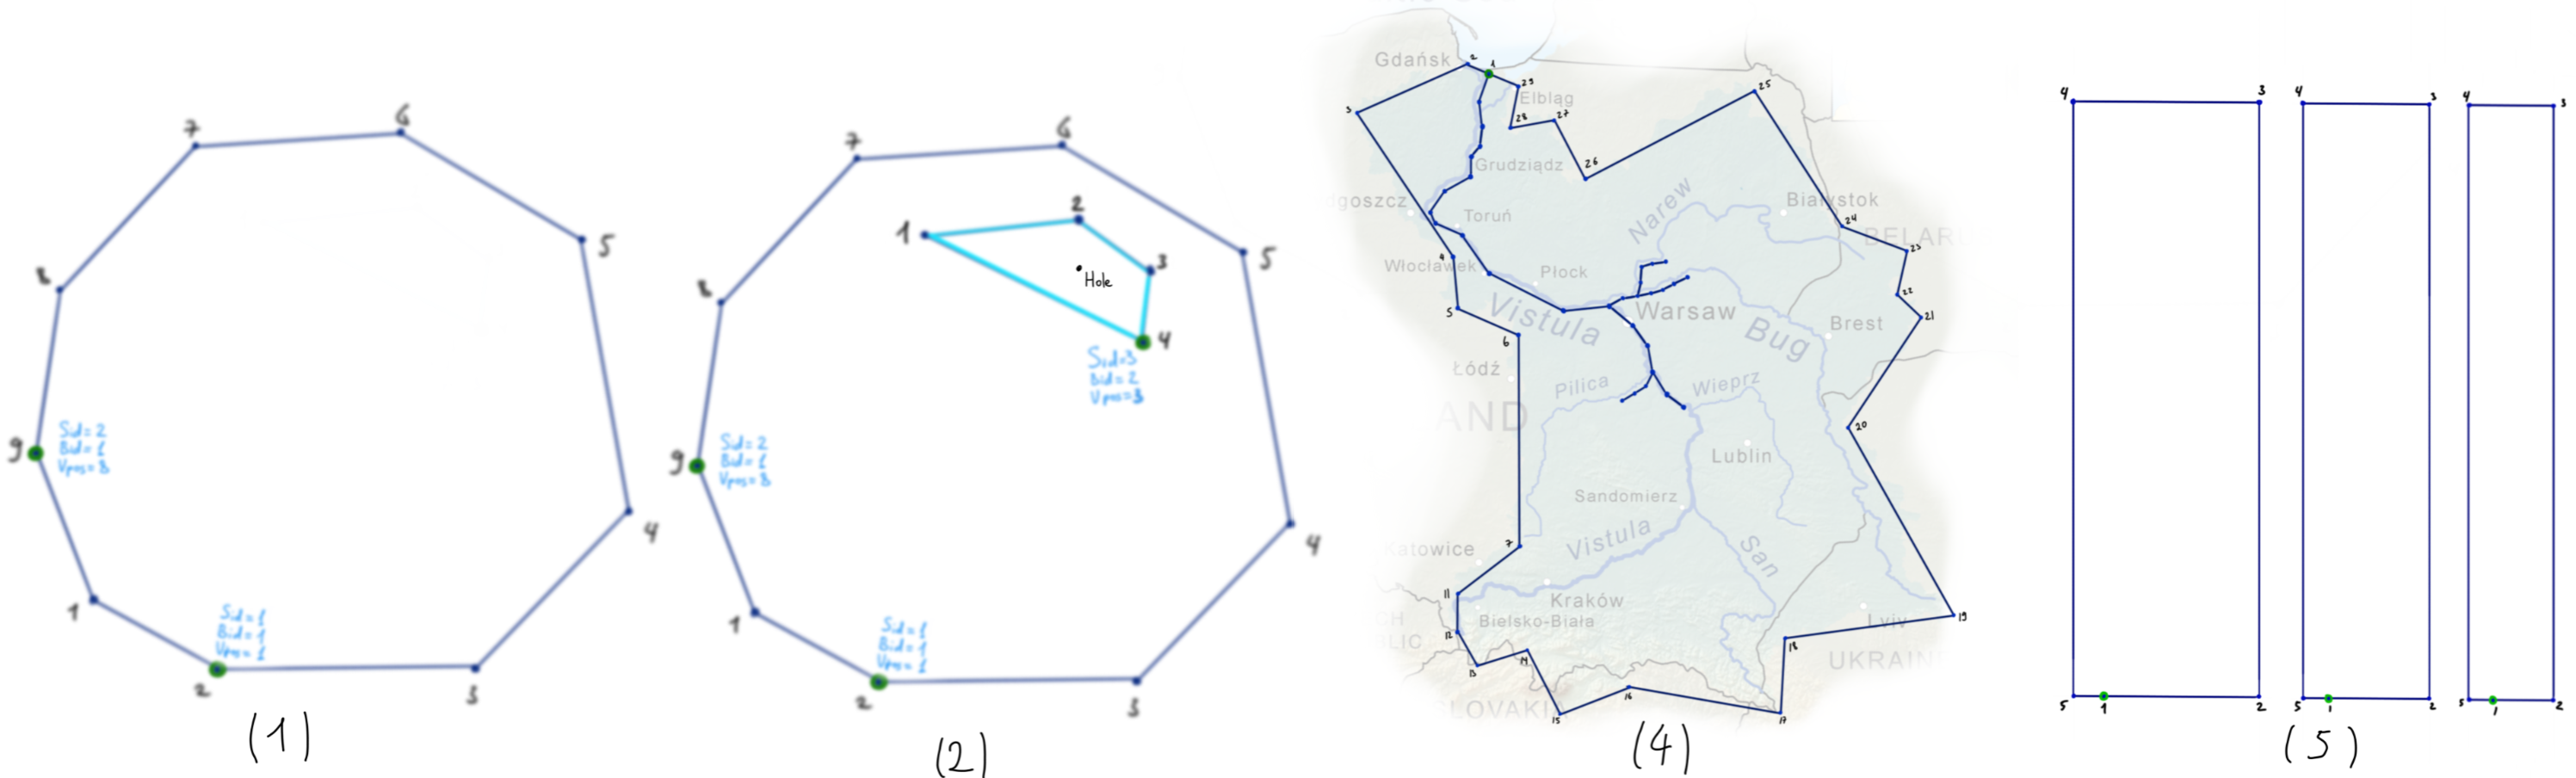
\includegraphics[width=1\textwidth]{figs/geometry_examples.png}
        %Szereg przykładów granicy:  brzeg z dwoma zaznaczonymi źródłami (1), granica zawierająca granicę(na przykład jezioro) (2), basen rzeki aproksymowany łamą linią i częściowo odzwierciedloną rżeką (4), dwa prostokąty z różną szerokością nie powiązane topologicznie(5).
        \caption{Examples of different domains: a boundary with two springs (1), a boundary containing a hole (for example, a lake) (2), a river basin approximated with the polygon and the river network (4), three domains not connected topologically which can be used for example to run several simulations with slightly different domains (5).}
        \label{geometry_examples}
      \end{figure}
      
      %І що б охопити всю цю довільність геометрії, було створено цілий ряд класів і функцій. Деякі найголовніші класи і функції: Point, Polar, Line, Boundary, BoundaryConditions, Sources, Branch, Rivers, Region і функція BoundaryGenerator. Приклади використання даних функцій розглянемо далі.
      %Aby pokryć całą tę arbitralność geometrii, stworzono szereg klas i funkcji\ref{GeometryClasses}. Niektóre z najważniejszych klas i funkcji to Point, Polar, Line, Boundary, BoundaryConditions, Sources, Branch, Rivers, Region i funkcja BoundaryGenerator. Poniżej rozważymy przykłady użycia tych funkcji.
      In order to cover all this arbitrariness of geometry, a number of classes and functions were created (Fig. \ref{GeometryClasses}). Some of the most important classes and functions are Point, Polar, Line, Boundary, BoundaryConditions, Sources, Branch, Rivers, Region, and the BoundaryGenerator function. We will consider examples of the use of these functions below.
      
      \begin{figure}[H]
        \centering
        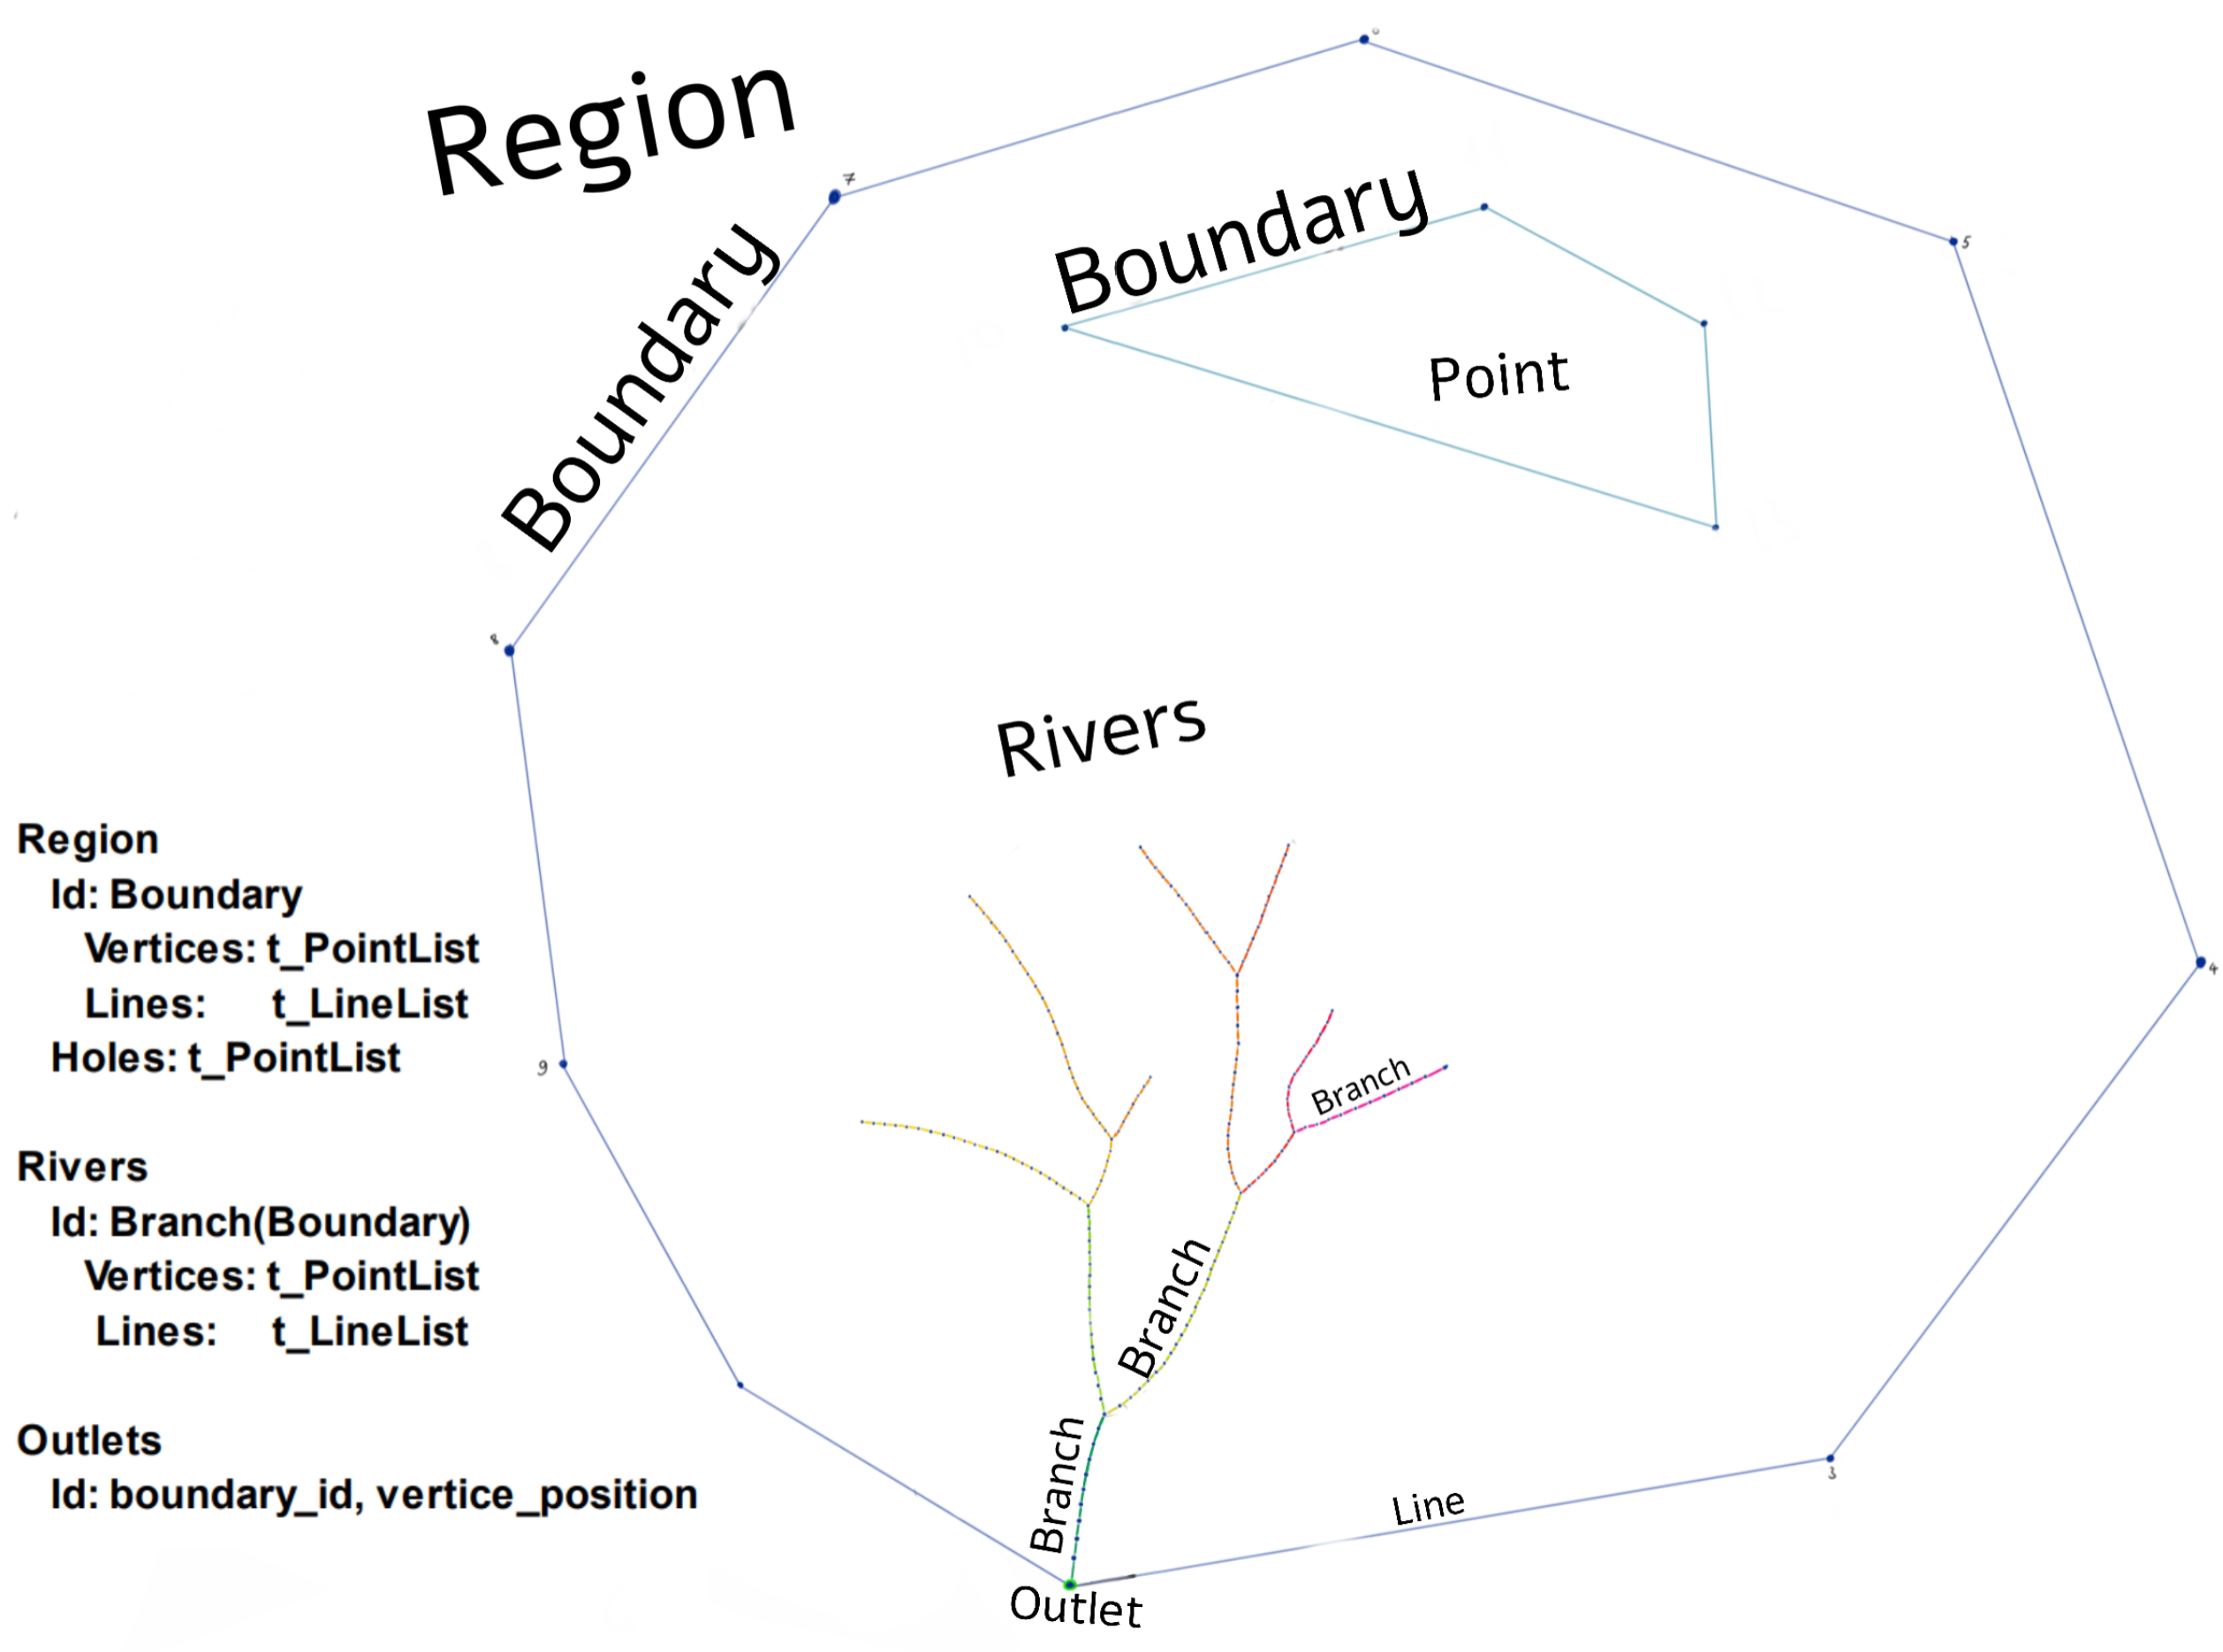
\includegraphics[width=0.7\textwidth]{figs/GeometryClasses.png}
        %Ilustracja objektów zdefiniowanych w bibliotece Riversim i ich relacje pomiędzy sobą przy konfigurowaniu geometrii.
        \caption{An illustration of objects defined in the Riversim library and their relationships to each other when configuring geometry.}
        \label{GeometryClasses}
      \end{figure}

      \begin{figure}[H]
        \centering
        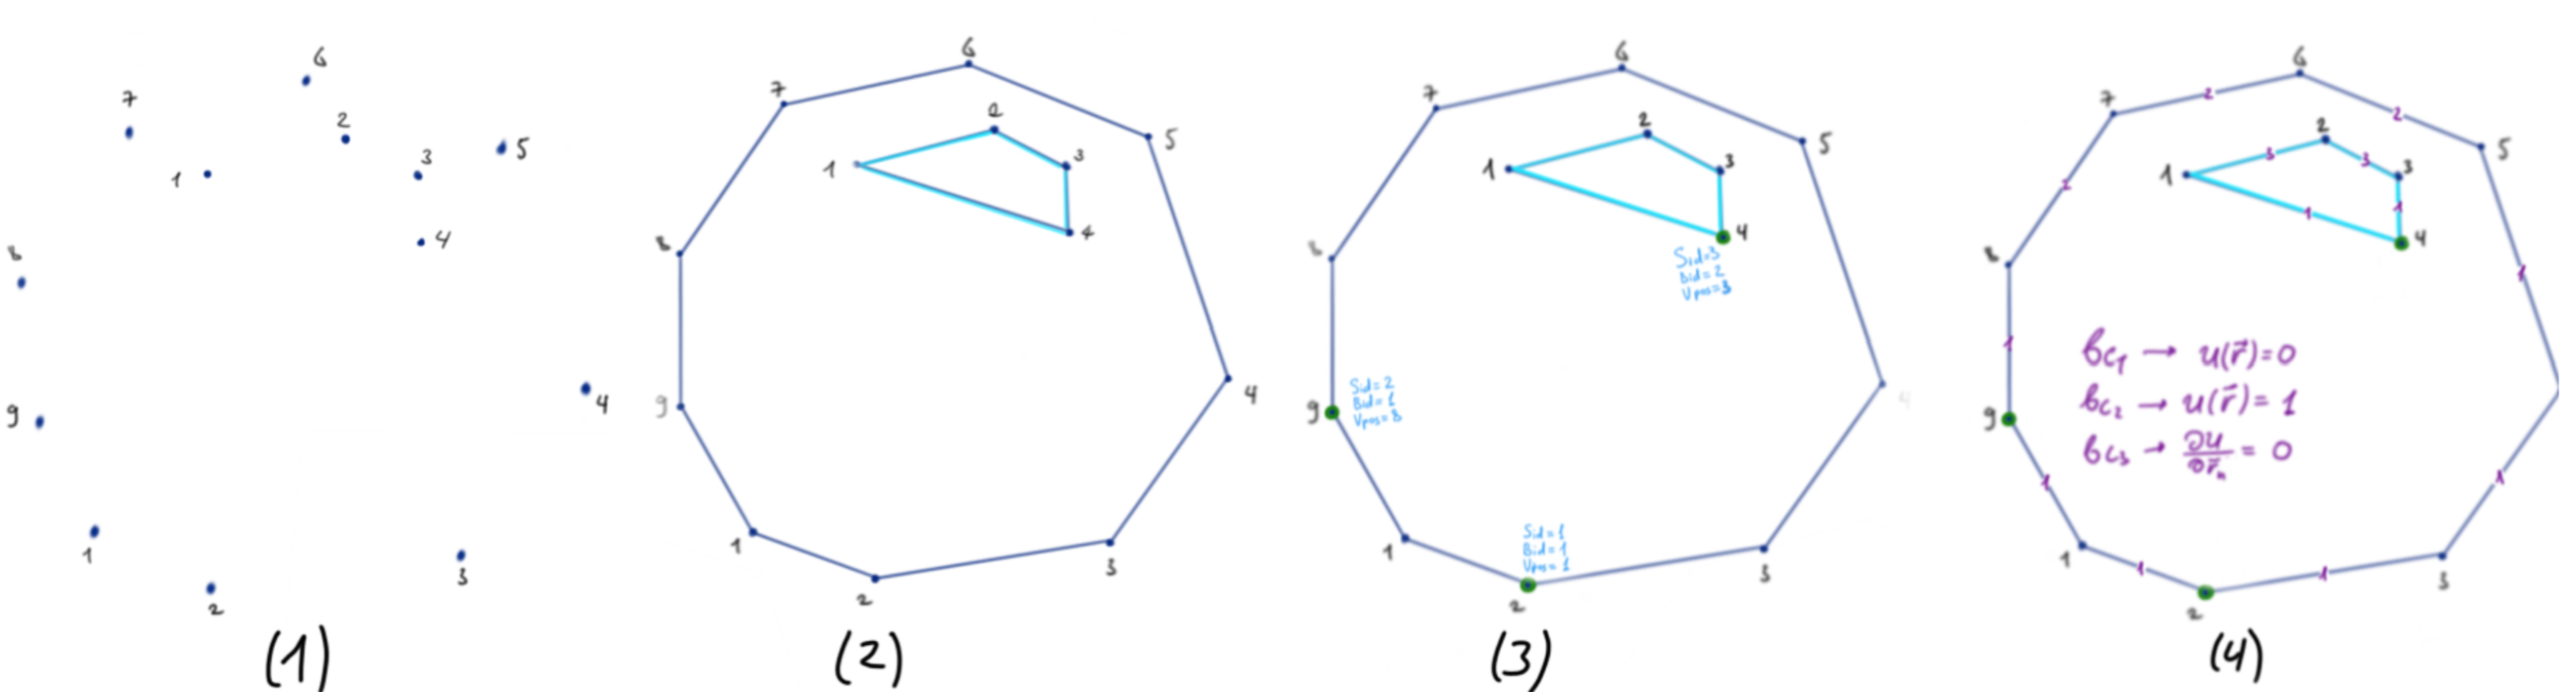
\includegraphics[width=0.9\textwidth]{figs/region_workflow.png}
        %Ilustracja kolejności kroków przy definicji regionu. Definicja wszystkich punktów i zapisanie ich do oddzielnychlist t\_PointList jeżeli należą do różnych brzegów (1). Definicja linii i indeksów i też przepisanie ich do oddzielnych list t\_LineList (2). Definicja punktów źródłowych na granicy w klasie spring (3). Definicja warunków brzegowych (4).
        \caption{Illustration of the sequence of steps in defining a region. Define all points and store them in separate lists t\_PointList if they belong to different edges (1). Definition of lines and indexes and rewriting them to separate lists t\_LineList (2). Definition of spring points on the boundary in the Source class (3). Definition of boundary conditions (4).}
        \label{region_workflow}
      \end{figure}

      %Спочатку задаємо впорядковану множину координат з допомогою класу Point і ліній з допомогою класу Line для визначення границі. В програмі границя репрезентується класом Boundary. Таких границь може бути декілька. Група границь котрим присвоєний унікальний індекс утворює регіон який репрезентується класом Region. Границя - це замкнута лінія, іншими словами полігон. В регіоні немає обмежень на кількість границь. Границя також може містити цілковито іншу границю, проте перетин ліній не допускається. Щоб утворити дірку в границі потрібно визначити координату в межах цієї границі і присвоїти до списку дір який зберігається в класі Region. Наступним кроком є визначення місць звідки буде відбуватися ріст мережі річки. Такими місцями може бути кожна  точка границі і джерел може бути необмежена кількість(практично обмежена сумарної кількістю координат границь). Для зберігання інформації про початкові координати джерел створено клас Source. Цей клас зберігає унікальний номер кожного джерела, номер границі на котрій розташовується і номер координати на даній границі.
      %Najpierw określamy uporządkowany zestaw współrzędnych za pomocą klasy Point i linii za pomocą klasy Line, aby określić granicę. W programie granica jest reprezentowana przez klasę Boundary. Takich granic może być kilka. Grupa granic, którym przypisano unikalny indeks, tworzy region reprezentowany przez klasę Region. Granica jest zamkniętą linią, innymi słowy wielokątem. W regionie nie ma ograniczeń co do liczby granic. Jedna granica może również zawierać inną granicę, ale przecięcie linii jest niedozwolone. Aby utworzyć otwór w granicy, należy zdefiniować współrzędną w obrębie tej granicy i przypisać ją do listy otworów przechowywanej w klasie Region. Kolejnym krokiem jest określenie miejsc, z których nastąpi rozwój sieci rzecznej. Takimi miejscami może być każdy punkt granicy, a źródeł może być nieograniczona (praktycznie ograniczona całkowitą liczbą współrzędnych granic). Klasa Source została stworzona do przechowywania informacji o początkowych współrzędnych źródeł. Ta klasa przechowuje unikalny numer każdego źródła, numer granicy, na której się znajduje, oraz numer współrzędnej na tej granicy.
      First, we specify an ordered set of coordinates using the Point class and lines using the Line class to determine the boundary. In the program, the boundary is represented by the Boundary class. There can be several such borders. A group of boundaries assigned a unique index forms a region represented by the Region class. The border is a closed line, in other words, a polygon. There are no limits on the number of borders in the region. The border can also contain a different border, but crossing lines is not allowed nor sharing common vertex. To create a hole in a border, you need to define a coordinate within this border and assign it to the list of holes stored in the Region class. The next step is to determine the places from where the growth of the river network will take place. Such places can be every point of the border and there can be an unlimited number of springs (practically limited by the total number of coordinates of the borders). The Source class was created to store information about the initial coordinates of the springs. This class stores the unique number of each spring, the number of the boundary on which it is located, and the number of the coordinate on this boundary (Fig. \ref{region_workflow}).

      \begin{mintedbox}{python}
        from riversim import *

        outer_boundary = Boundary()
        outer_boundary.vertices.extend([Point(0.13, 0.011), Point(0.31, 0), Point(0.74, 0.15), Point(0.95, 0.35), Point(0.8, 0.75), Point(0.47, 0.85), Point(0.152, 0.76), Point(0, 0.5), Point(0.025, 0.3)])
        outer_boundary.lines.extend([Line(0, 1, 1), Line(1, 2, 1), Line(2, 3, 1), Line(3, 4, 1), Line(4, 5, 2), Line(5, 6, 2), Line(6, 7, 1), Line(7, 8, 1), Line(8, 0, 1)])

        inner_boundary = Boundary()
        inner_boundary.vertices.extend([Point(0.3, 0.7), Point(0.5, 0.76), Point(0.65, 0.7), Point(0.66, 0.59)])
        inner_boundary.lines.extend([Line(0, 1, 1), Line(1, 2, 3), Line(2, 3, 3), Line(3, 0, 1)])

        region = Region()
        region[1] = outer_boundary; region[2] = inner_boundary
        region.holes.append(Point(0.4, 0.7))

        sources = Sources()
        sources[1] = t_source_coord(1, 1) 
        sources[2] = t_source_coord(1, 8) 
        sources[3] = t_source_coord(2, 3)\end{mintedbox}

      %Після визначення регіону і розташування джерел, тепер можемо перейти до побудови геометрії річки. Всі дані про геометрію річок і алгоритми містяться в класі Rivers. Rivers містить унікальний номер для кожної річки, котрий має теж саме значення,  що й номер джерела в Sources. Для ініціалізації класу Rivers, потрібно конвертувати дані з класу Sources в координати і напрямок. Для цього служить функція GetSourcesIdsPointsAndAngles класу Region аргументом котрої є Sources. В результаті ми отримаємо набір індексів річок і відповідні їм координати і напрямок перпендикулярний до границі. Для визначення точного напрямку перпендикуляру, має значення напрямок координати при задаванні границі. Прийнято, що перпендикуляр буде з лівої сторони від напрямку координат. Тому якщо звернути увагу на регіон де є дірка по центрі, то зовнішня границя має протилежний напрямок нумерації координат відносно внутрішньої.
      %Po określeniu regionu i lokalizacji źródeł możemy przystąpić do konstruowania geometrii rzeki. Wszystkie dane geometrii rzeki i algorytmy są zawarte w klasie Rivers. Rzeki zawierają unikalny numer dla każdej rzeki, który ma takie samo znaczenie jak numer źródła w Źródłach. Aby zainicjować klasę Rivers, należy przekonwertować dane z klasy Sources na współrzędne i kierunek. W tym celu jako argument służy funkcja GetSourcesIdsPointsAndAngles klasy Region, której argumentem jest Sources. W rezultacie otrzymamy zestaw indeksów rzecznych i odpowiadających im współrzędnych oraz kierunek prostopadły do granicy. Aby określić dokładny kierunek prostopadłej, podczas wyznaczania granicy ważny jest kierunek współrzędnych. Zakłada się, że prostopadła będzie po lewej stronie kierunku współrzędnych. Dlatego jeśli zwrócisz uwagę na obszar, w którym znajduje się dziura w środku, wówczas zewnętrzna granica ma przeciwny kierunek numeracji współrzędnych w stosunku do wewnętrznej.
      After determining the region and the location of the springs, we can now proceed to the construction of the geometry of the river. All river geometry data and algorithms are contained in the Rivers class. Rivers contains a unique number for each river, which has the same value as the spring number in Sources. To initialize the Rivers class, you need to convert the data from the Sources class into coordinates and nomal vector (Fig. \ref{rivers_initialization}). For that purpose the GetSourcesIdsPointsAndAngles function of the Region class is used, which has Sources as its argument. As a result, we will get a set of river indices and their corresponding coordinates and the normal vectors to the border. To determine the normal vector dirrection, order of the coordinate is important when setting the border. It is assumed that the perpendicular will be on the left side of the coordinate order. Therefore, if you pay attention to the region where there is a hole in the center, then the outer border has the opposite order of coordinate numbering relative to the inner one.
      
      \begin{figure}[H]
        \centering
        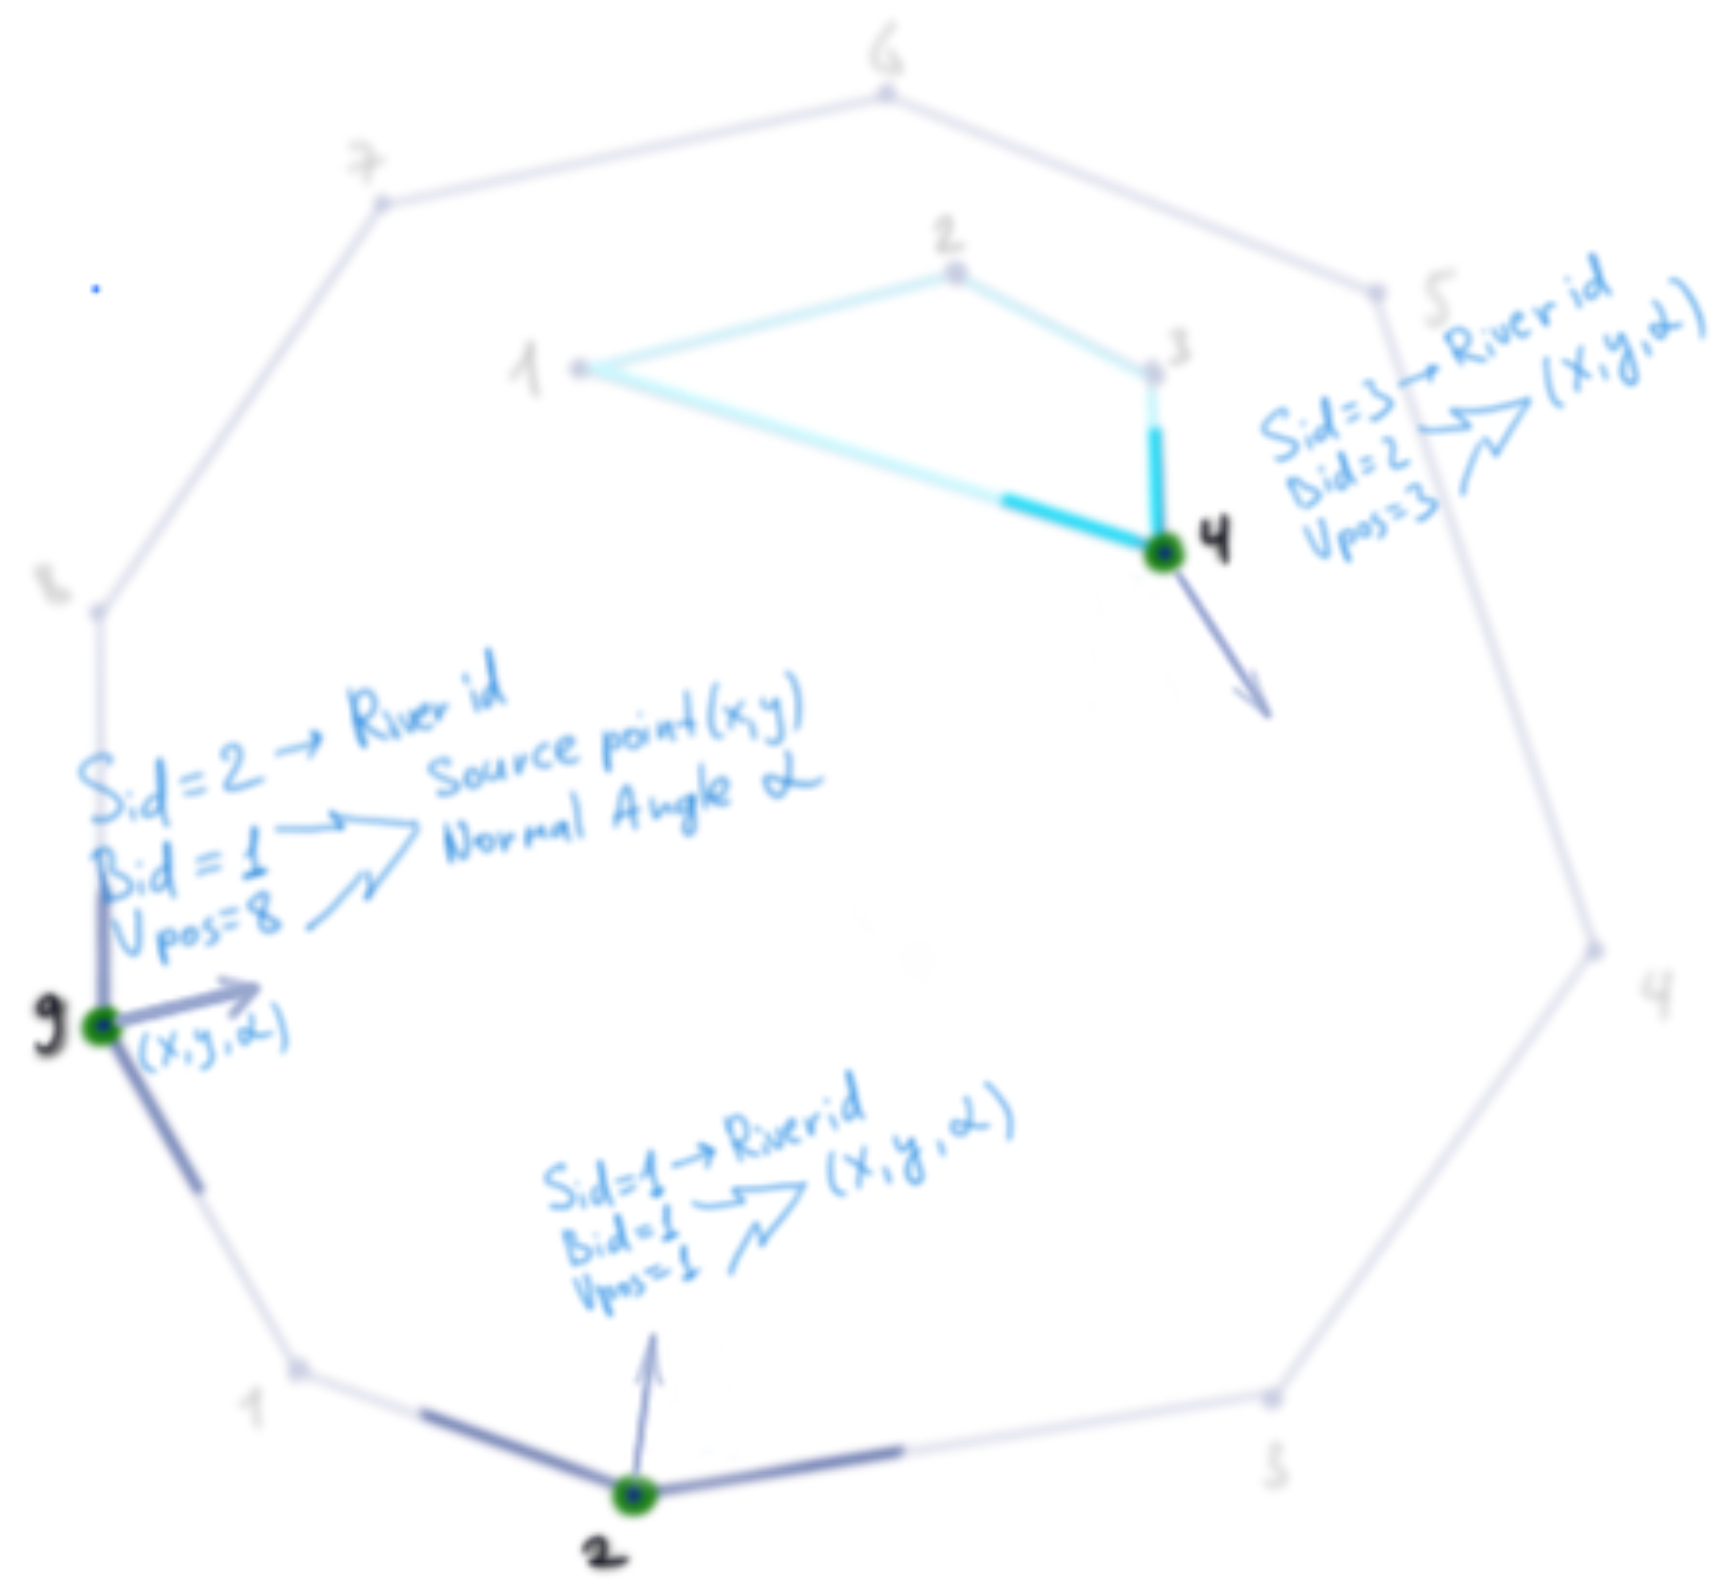
\includegraphics[width=0.6\textwidth]{figs/rivers_initialization.png}        
        %Indeksy brzegów i odpowiednich współrzędnych, które są przechowywane w klasie Source, są konwertowane w współrzędne i kąt normalnej linii w danym punkcie granicy. Te dane są wykorzystywane dla inicjalizacji struktury Rivers która przechowuje dane o sieci rzecznej.
        \caption{The boundary and corresponding coordinate indexes, which are stored in the Source class, are converted to the coordinates and angle of the normal line at the given boundary point. This data is used to initialize the Rivers structure which holds data about the river network.}
        \label{rivers_initialization}
      \end{figure}

      \begin{mintedbox}{python}
        rivers = Rivers()
        rivers.initialize(region.getSourcesIdsPointsAndAngles(sources))\end{mintedbox}
      
      %Вище вказувалося, що в більшості випадків біфуркація річки відбувається на дві частини. А якщо поділів відбувається більше, ми можемо вважати це двома послідовними достатньо близько розташованими між собою біфуркаціями. Поміж біфуркаціями річка апроксимується ламаною лінією. Інформація  про цю лінію криється в класі Branch. А інформація про те котрі частини річки з'єднуються з іншими частинами річки в пунктах біфуркації міститься в графі котрий в свою чергу міститься в класі Rivers. Класс Rivers надає можливості для легкого способу працювати із геометрією річки, а саме: отримання інформації про поточний стан річок(довжини, відношення між частинами річками, визначення кривизни, координати джерел і тд), розвиток мережі річки(додавання нових координат до річки при рості, згладжування кривизни, створення нових річок, додавання нових пунктів біфуркації), зменшення довжини річки і  видалення пунктів біфуркації для полегшення обрахунків при оберненій еволюції. 
      %Powyżej zaznaczono, że w większości przypadków rzeka rozdziela się na dwie części. A jeśli podziałów jest więcej, możemy to uznać za dwa kolejne bifurkacje dostatecznie blisko siebie. Pomiędzy punktami bifurkacji rzeka jest aproksymowana linią przerywaną. Informacje o tej linii znajdują się w klasie Branch. A informacja o tym, które odcinki rzeki łączą się z innymi odcinkami rzeki w punktach rozwidlenia, zawarta jest w grafie, który z kolei jest zawarty w klasie Rivers. Klasa Rivers daje możliwość łatwej pracy z geometrią rzek, a mianowicie: uzyskiwania informacji o aktualnym stanie rzek (długości, relacje między odcinkami rzek, określanie krzywizny, współrzędne źródeł itp.), opracowywania sieci rzecznej ( dodawanie nowych współrzędnych do rzeki podczas wzrostu, wygładzanie krzywizny, tworzenie nowych rzek, dodawanie nowych punktów bifurkacji), zmniejszanie długości rzeki i usuwanie punktów bifurkacji w celu ułatwienia obliczeń podczas ewolucji odwrotnej.
      It was indicated above that in most cases at the bifurcation points river divides into two parts. And if there are more divisions, we can consider it as two successive bifurcations sufficiently close to each other. Between the bifurcations, the river is approximated by a broken line. Information about this line lies in the Branch class. And the information about which parts of the river connect with other parts of the river at bifurcation points is contained in the Rivers class. The Rivers class provides methods for an easy way to work with river geometry, namely: obtaining information about the current state of rivers (lengths, relationships between parts of rivers, determining curvature, coordinates of springs, etc.), developing a river network (adding new coordinates to a river when growing, smoothing the curvature, creating new rivers, adding new bifurcation points), reducing the length of the river and removing bifurcation points to facilitate calculations in reverse evolution.
      
      \begin{mintedbox}{python}
        rivers_ids = t_sources_ids(); rivers_ids.extend([1, 2, 3])
        ds = 0.01
        tip_points = t_PolarList(); tip_points.extend([Polar(ds, 0), Polar(ds, 0), Polar(ds, 0)])
        boundaries_ids = t_boundaries_ids(); boundaries_ids.extend([1, 2, 1])
        rivers.addPolars(rivers_ids, tip_points, boundaries_ids)
      
        sub_branch_ids = rivers.createSubBranches(1, -3.1415/5, 3.1415/5)\end{mintedbox}

      %Оскільки мережа річки котра міститься в класі Rivers опирається в своїй реалізації на клас Boundary, то для кожного сегменту річки ми можемо задати унікальні граничні умови. Наприклад, можна врахувати "опір" русла ріки і збільшення висоти підземних вод вздовж.
      %Ponieważ sieć rzeczna zawarta w klasie Rivers opiera się w swojej implementacji na klasie Boundary, możemy ustawić unikalne warunki brzegowe dla każdego odcinka rzeki. Naprzykład, możemy uwzględnić „opór” koryta rzeki i wzrost wysokości wód gruntowych wzdłuż niego.
      Since the river network contained in the Rivers class is based on the Boundary class, we can set unique boundary conditions for each segment of the river. For example, it is possible to take into account the "resistance" of the river bed and the increase in the height of groundwater along it. So, we can remove assumption that groundwater level $\phi$ is equal to zero on its entire length and assign unique boundary index for each segment which corresponds to different groundwater table height ($\phi(i) \sim i$, where $i$ is segment number).

      \begin{figure}[H]
        \centering
        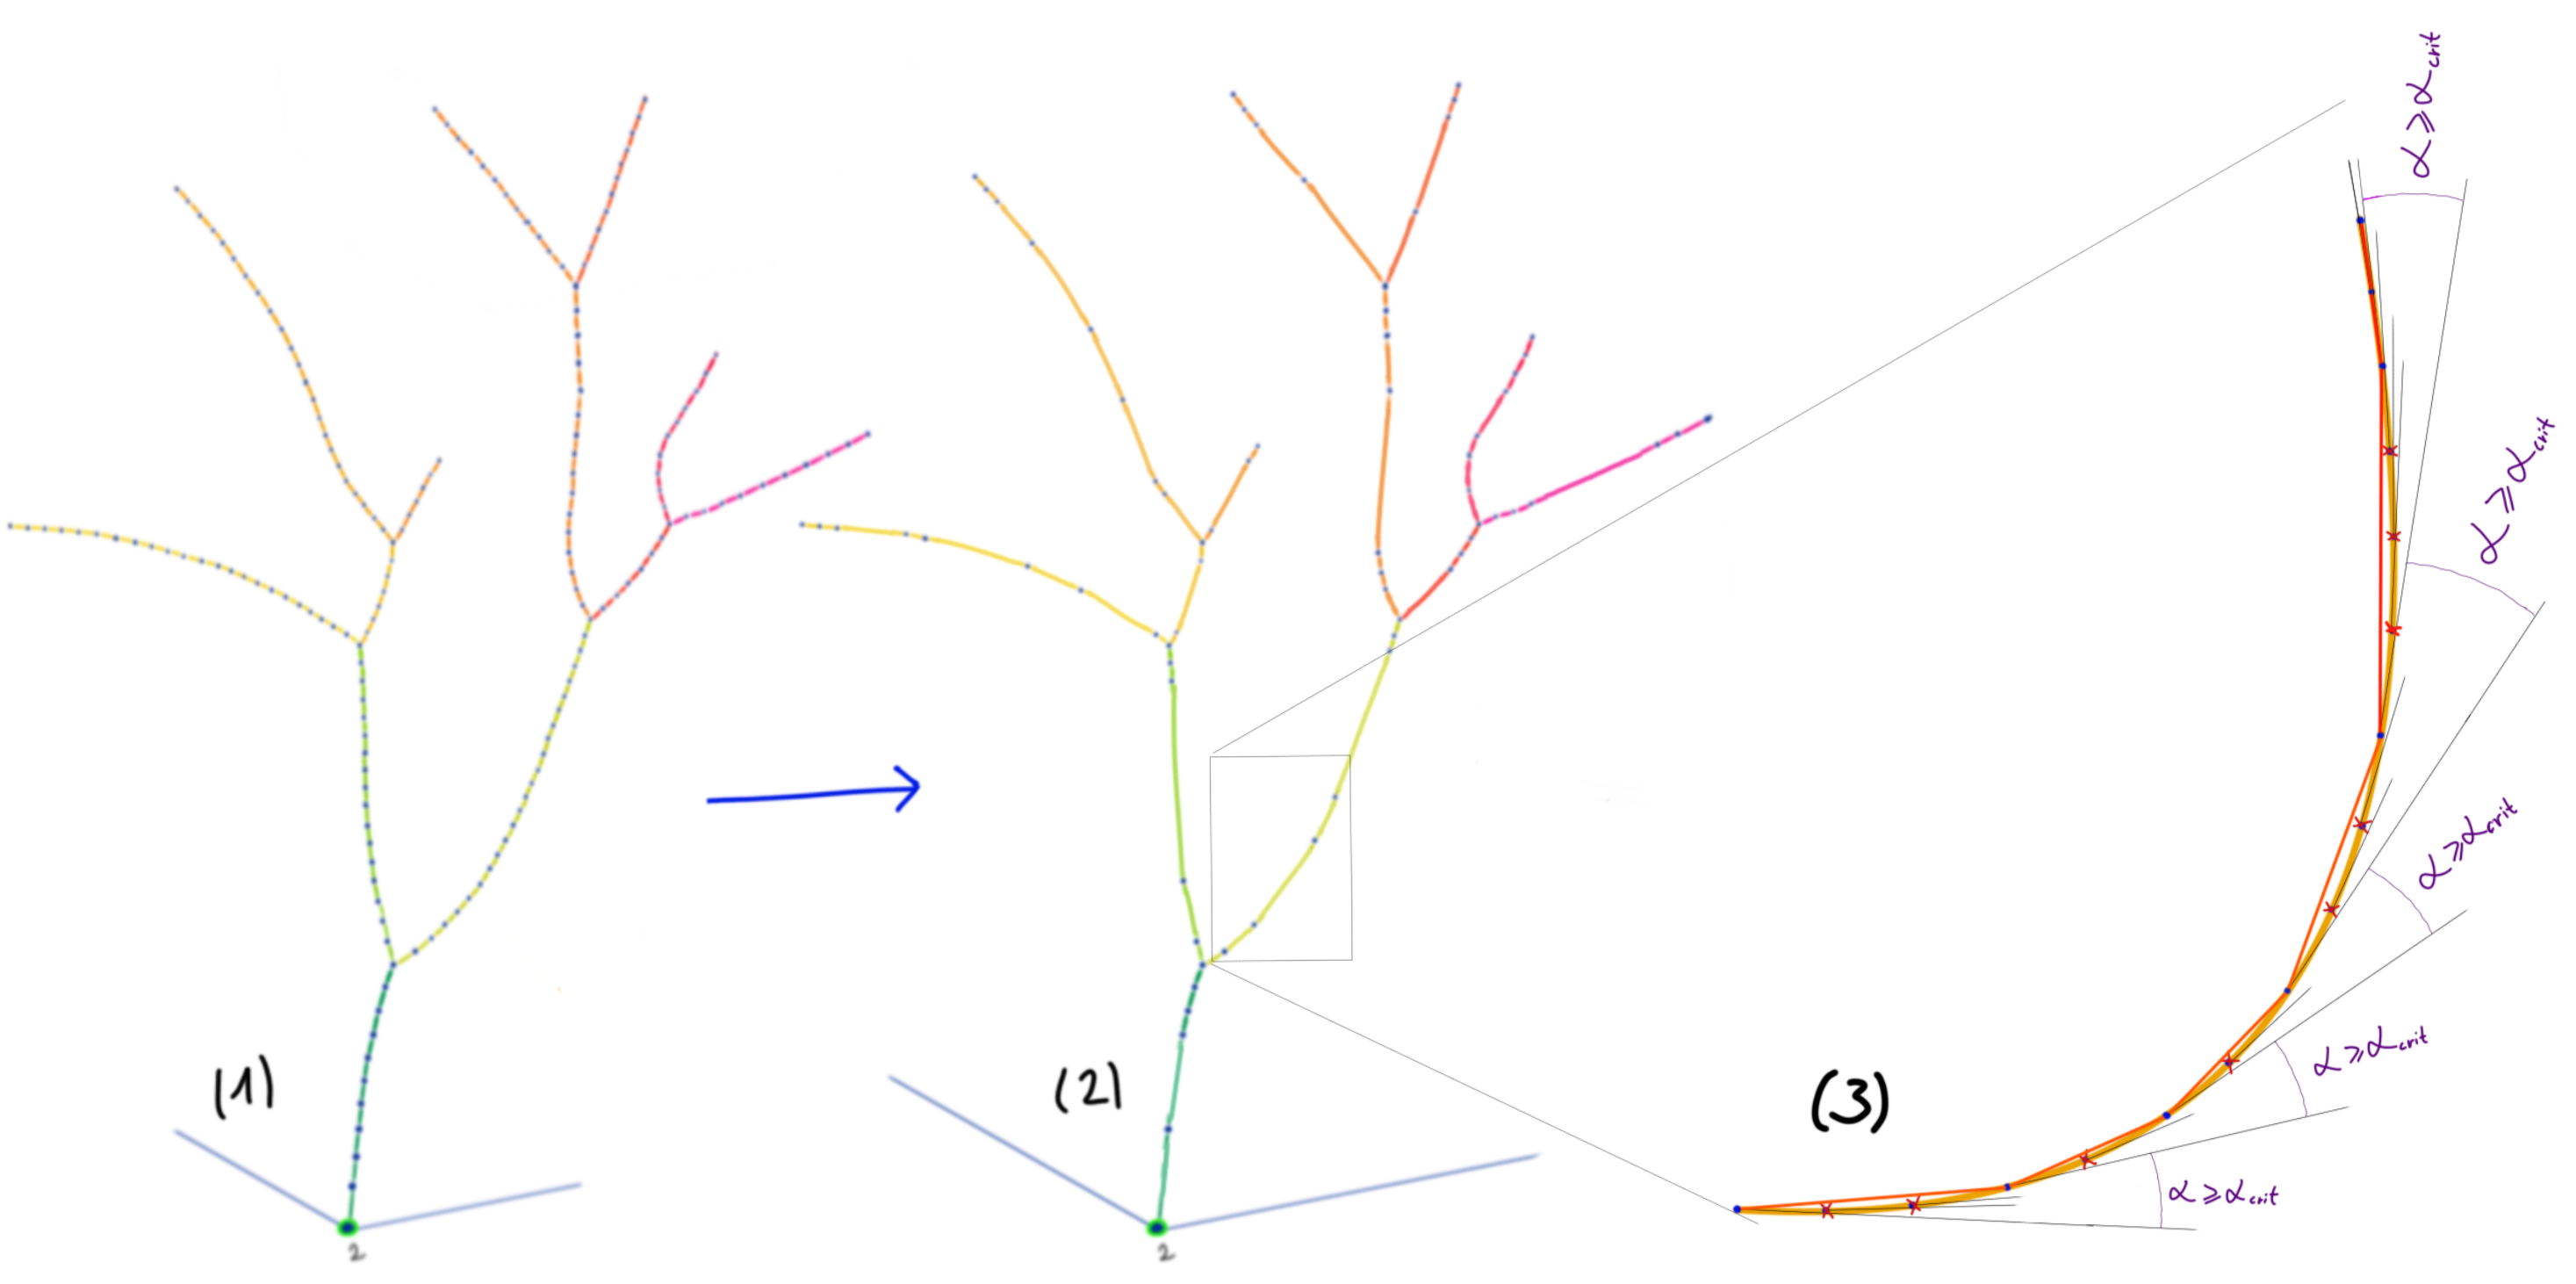
\includegraphics[width=0.9\textwidth]{figs/tree_coarsening.png}        
        %Ilustracja zmniejszenia gęstości współrzędnych na granicy przy zachowaniu wystarczającej dokładności.
        \caption{Illustration of reducing the coordinate density at the boundary while maintaining sufficient accuracy.}
        \label{tree_coarsening}
      \end{figure}

      %Кількість елементів сітки на котру ми розділюємо регіон має прямий вплив на розмір матриці лінійних рівняння, а тому на час знаходження розв'язку диференційного рівняння. Щоб зменшити час обчистленнь, ми можемо зменшити густини координат границі річки, при цьому не втрачаючи на точності. Для цього ми робимо процедуру огрублення границь частин річки. Тепер нам потрібно класи  Sources, Region та Rivers вкласти в границю Boundary, оскільки генератор сітки вимагає тільки  границю як аргумент. Другою проблемою, котра згадувалася вище є те, що немає можливості задати граничні умови в середині регіону, а тільки на границі. Для цього лінії з котрих складається мережа річки розділяються на дві лінії котрі знаходяться дуже близько одна до одної.
      %Liczba elementów siatki, na jakie dzielimy obszar, ma bezpośredni wpływ na wielkość macierzy równań liniowych, a więc na czas znalezienia rozwiązania równania różniczkowego. Aby skrócić czas obliczeń, możemy zmniejszyć gęstość współrzędnych granicy rzeki bez utraty dokładności. Zmniejszenie zagęszczenia współrzędnych na granicy opiera się na następującej idei: każda kolejna współrzędna zmienia kierunek linii o pewien kąt. Jeśli kąt jest bardzo mały, możemy założyć, że współrzędne leżą praktycznie na tej samej linii. Dlatego możemy usunąć wszystkie współrzędne pośrednie i pozostawić tylko te skrajne. Aby znaleźć „skrajne” współrzędne linii, iterujemy po wszystkich współrzędnych i obliczamy całkowity kąt odchylenia, gdy tylko ten kąt stanie się większy niż wartość krytyczna, traktujemy tę współrzędną jako skrajną.
      The number of grid elements into which we divide the region has a direct effect on the size of the matrix of linear equations, and therefore on the time of finding the solution of the differential equation. To reduce the solution time, we can reduce the density of the coordinates of the river border without losing much of accuracy (Fig. \ref{tree_coarsening}). For this purpose, we perform the procedure of roughing the borders of parts of the river. 
      %Now we need to nest the Sources, Region, and Rivers classes in the Boundary boundary since the mesh generator requires only the boundary as an argument. The second problem, which was mentioned above, is that there is no possibility to set boundary conditions in the middle of the region, but only on the border. For this, the lines that make up the river network are divided into two lines that are very close to each other.

    \section{Mesh generation}

      \begin{figure}[H]
        \centering
        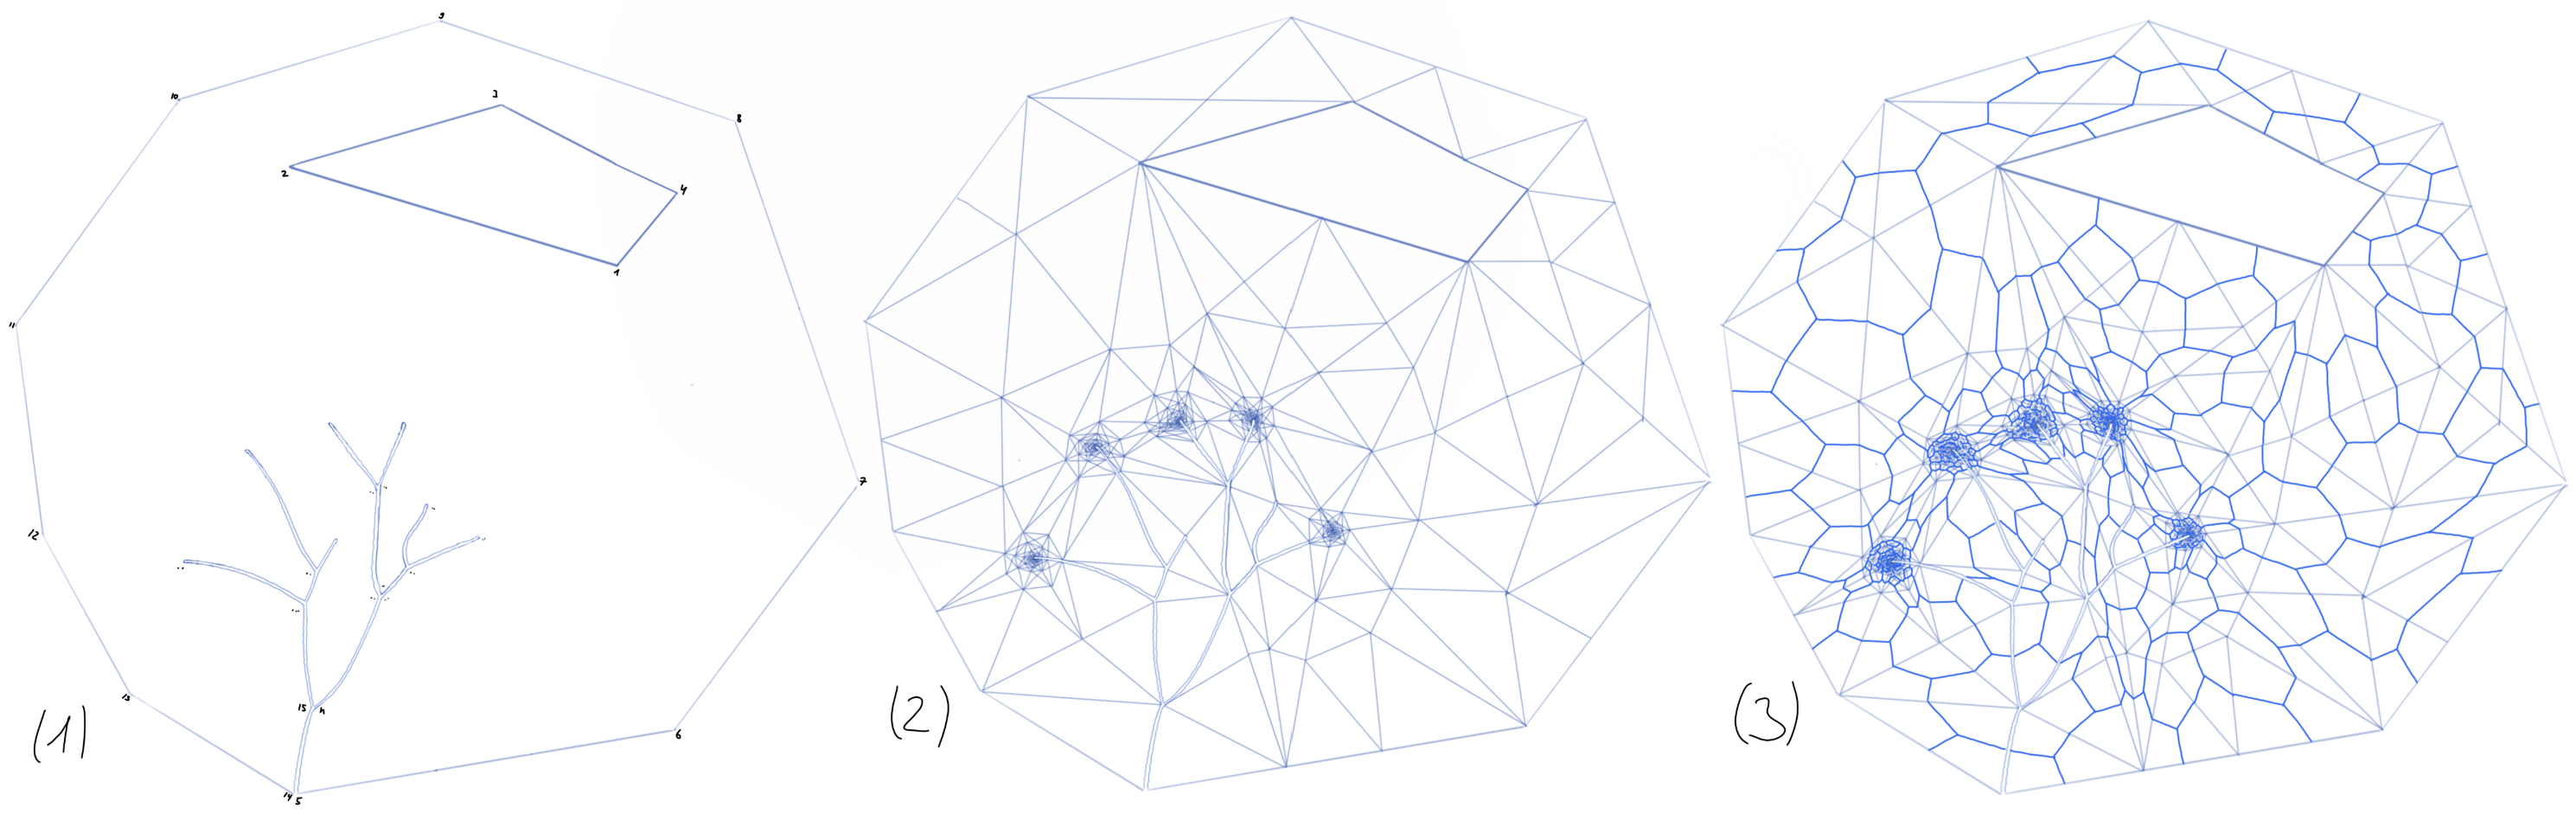
\includegraphics[width=0.9\textwidth]{figs/mesh_generation.png}        
        %Wszystkie brzegi które są zawierane w klasie Region, a także brzegi rzek w klasie Rivers łączą się w jeden zamknięty brzeg (1). Z pomocą Triangle na bazie jednej zamkniętej granicy jest generowana siatką trójkątowa (2). Siatka trójkątowa z pomocą biblioteki Tethex jest konwertowana w siatkę prostokątów (3).
        \caption{All boundaries that are contained in the Region class, as well as river boundaries in the Rivers class are merged into one closed boundary (1). With the help of a Triangle, a triangular mesh (2) is generated on the basis of one closed border. A triangular mesh is converted into a rectangular mesh with the help of the Tethex library (3).}
        \label{mesh_generation}
      \end{figure}

      %Для генерації сітки нам потрібна замкнута границя Boundary. Для цього існує функція BoundaryGenerator, котра об'єднує класи  Sources, Region та Rivers в одну границю Boundary. Другою проблемою, котра згадувалася вище є те, що немає можливості задати граничні умови в середині регіону, а тільки на границі. Для цього лінії з котрих складається мережа річки розділяються на дві лінії котрі знаходяться достатньо близько одна до одної.
      %Aby wygenerować siatkę, potrzebujemy zamkniętej granicy Boundary. W tym celu dostępna jest funkcja BoundaryGenerator, która łączy klasy Sources, Region i Rivers w jedną granicę Boundary. Drugi problem, o którym była mowa powyżej, polega na tym, że nie ma możliwości ustalenia warunków brzegowych w środku regionu, a jedynie na granicy. W tym celu linie tworzące sieć rzeczną są podzielone na dwie linie, które są wystarczająco blisko siebie.
      To create a grid, we need a closed Boundary. For this, there is a BoundaryGenerator function that combines the Sources, Region, and Rivers classes into a single Boundary boundary. The second problem mentioned above is that it is not possible to set boundary conditions in the middle of the region, only on the boundary. For this, the lines that make up the river network are converted into two parallel lines, located quite close to each other(Fig. (1) \ref{mesh_generation}).

      \begin{mintedbox}{python}
        region_params = RegionParams()
        region_params.smoothness_degree = 0.2
        region_params.river_width = 1e-8
        boundary = BoundaryGenerator(sources, region, rivers, region_params)\end{mintedbox}

      %Коли є замкнута границя можна згенерувати сітку. Для цього була використана C++ бібліотека \cite{szewczuk1996triangle}. Методи і алгоритми бібліотеки Traingle містяться в однойменному класі. Triangle генерує Деланау сітку. Triangle дає можливість задати значення мінімального кута трикутника, мінімальної і максимальної довжини сторони трикутника, мінімальної і максимальної площі трикутника, співвідношення сторін трикутника та інше. Другим важливим аспектом є генерація достатньо малої сітки в місцях, де поле підземних вод змінюється найшвидше -- довкола джерел. Для цього можна задати множину координат(а саме координат джерел), де буде обмежена радіально площа трикутника відносно даних точок. Функція котра обмежує площу трикутника виглядає наступним чином:
      %Gdy istnieje zamknięta granica, można wygenerować siatkę. W tym celu wykorzystano bibliotekę C++ Triangle\cite{szewczuk1996triangle}. Metody i algorytmy biblioteki Traingle są zawarte w klasie o tej samej nazwie. Trójkąt generuje siatkę Delaunaya. Trójkąt pozwala ustawić wartość minimalnego kąta trójkąta, minimalną i maksymalną długość boku trójkąta, minimalną i maksymalną powierzchnię trójkąta, stosunek boków trójkąta itp. Drugim ważnym aspektem jest generowanie odpowiednio małej siatki w miejscach, w których pole wód podziemnych zmienia się najszybciej - w okolicach źródeł. Aby to zrobić, możesz określić zestaw współrzędnych (czyli współrzędne źródeł), w których obszar trójkąta względem danych punktów będzie ograniczony promieniowo. Funkcja ograniczająca pole trójkąta wygląda następująco:
      When there is a closed border, you can generate a grid (Fig. (2) \ref{mesh_generation}). For this, the Triangle C++ library \cite{szewczuk1996triangle} was used. The methods and algorithms of the Triangle library are contained in the class of the same name. Triangle generates a Delaunay mesh. Triangle allows you to set the value of the minimum angle of the triangle, the minimum and maximum length of the side of the triangle, the minimum and maximum area of the triangle, the ratio of the sides of the triangle, etc. The second important aspect is the generation of a sufficiently small grid in places where the groundwater field changes the fastest - around springs. To do this, you can specify a set of coordinates (namely, the coordinates of the springs), where the area of the triangle relative to the given points will be limited radially. The function that limits the area of the triangle looks like this:
      \begin{equation}
        A(r) = A_{min} + (A_{max} - A_{min}) \frac{1 - \exp{(\frac{-(\frac{r}{r_{ref}})^{e}}{2 \sigma^2})}}{1 + \exp{(\frac{-(\frac{r}{r_{ref}})^{e}}{2 \sigma^2})}} 
      \end{equation}

      Where $A_{min}$ -- is the minimal mesh area, $A_{max}$ -- the maximal mesh area, $r_{ref}$ -- specifies charatcterstic radius of transition, $\sigma$ and $e$ are responsible for slope of transiotion.

      %Розв'язувач Deal.II\cite{dealII94} вимагає сітки із квадратними елементами. Для цього ми використовуємо бібліотеку C++  Tethex \cite{tethex}  котра конвертує трикутні елементи сітки у чотирикутники, розбиваючи один трикутний елемент на три квадратних, чим збільшуючи кількість елементів сітки у три рази.
      %Solver Deal.II\cite{dealII94} wymaga siatki z elementami kwadratowymi. W tym celu używamy biblioteki Tethex \cite{tethex} C++, która konwertuje trójkątne elementy siatki na czworoboki, dzieląc jeden trójkątny element na trzy kwadratowe, zwiększając w ten sposób liczbę elementów siatki trzykrotnie.
      The Deal.II\cite{dealII94} solver requires a mesh with quadrilateral elements. For this, we use the Tethex C++ library \cite{tethex} , which converts triangular grid elements into quadrilaterals, dividing one triangular element into three square ones, thereby increasing the number of grid elements by three times (Fig. (3) \ref{mesh_generation}).

      \begin{mintedbox}{python}
        mesh_params = MeshParams()
        mesh_params.max_area = 1e6
        mesh_params.min_area = 6e-7
        mesh_params.max_edge = 1
        mesh_params.min_edge = 8e-12
        mesh_params.ratio = 2.3
        mesh_params.refinment_radius = 5e-3
        mesh_params.exponant = 1
        mesh_params.sigma = 1.9
      
        triangle = Triangle(mesh_params)
        triangle.mesh_params.tip_points = rivers.TipPoints()
        mesh = triangle.generate(boundary, region.holes)\end{mintedbox}

    \section{Boundary conditions}

      %Кожна лінія містить також номер(посилання) граничної умови. Boundaries -- клас котрий містить набір пар із унікальним номером і відповідною йому граничною умовою котра може бути двох типів: Діріхлет і Ноймана. Граничну умову можна задати тільки на граничній лінії, іншими словами задати лінію посеред регіону і граничну умову на ній не можна. Проте лінію завжди можна апроксимувати дуже тонким прямокутником, тож за потреби це не є проблемою.
      %Każda linia zawiera również numer (odniesienie) warunku brzegowego. Boundaries -- klasa zawierająca zbiór par o unikalnym numerze i odpowiadającym mu warunku brzegowym, który może być dwojakiego rodzaju: Dirichlet i Neumann. Warunek brzegowy można ustawić tylko na linii granicznej, innymi słowy, nie można ustawić linii pośrodku regionu i warunku brzegowego na nim. Jednak linię zawsze można przybliżyć bardzo cienkim prostokątem, więc w razie potrzeby nie stanowi to problemu.
      Each line also contains the number (reference) of the boundary condition. Boundaries -- is a class that contains a set of pairs with a unique number and the boundary condition corresponding to it, which can be of two types: Dirichlet and Neumann. The boundary condition can be set only on the boundary line, in other words, you cannot set a line in the middle of the region and a boundary condition on it. However, the line can always be approximated by a very thin rectangle, so this is not a problem if needed.

      \begin{mintedbox}{python}
        boundary_conditions = BoundaryConditions()
        boundary_conditions[1] = BoundaryCondition(DIRICHLET, 0)
        boundary_conditions[2] = BoundaryCondition(NEUMAN, 0)
        boundary_conditions[3] = BoundaryCondition(NEUMAN, 1)\end{mintedbox}

    \section{Groundwater potential profiles}

      \begin{figure}[H]
        \centering
        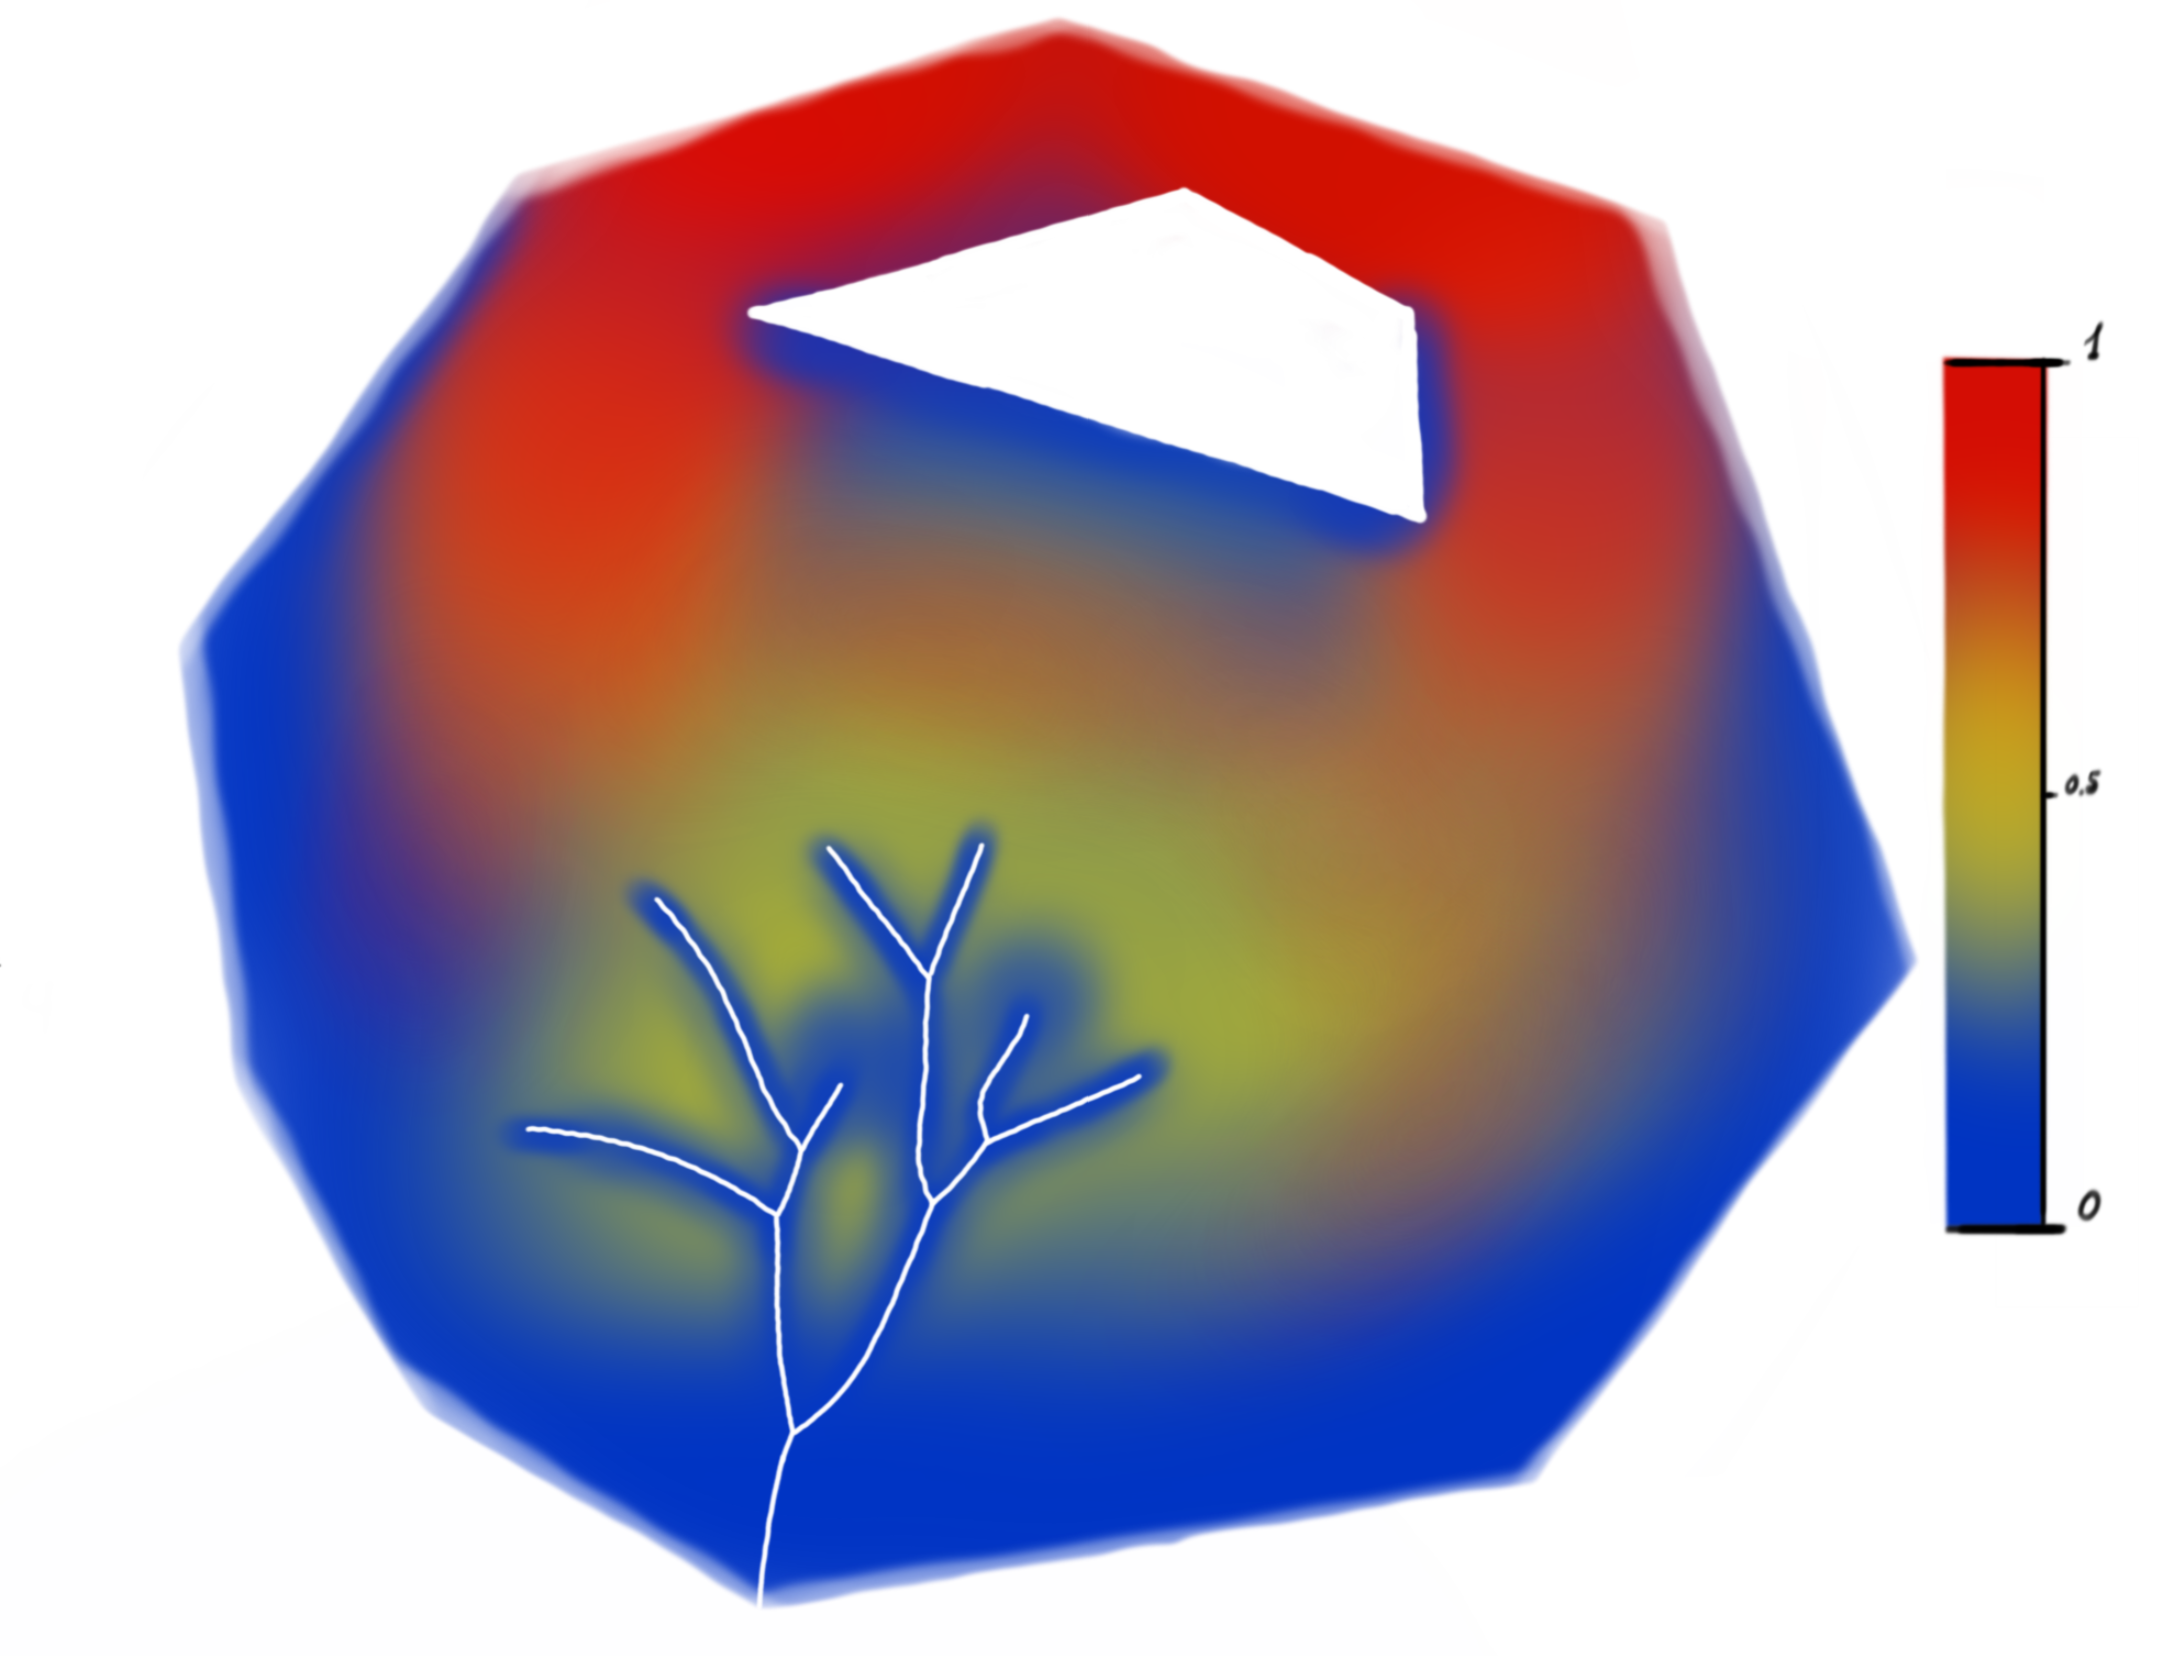
\includegraphics[width=0.9\textwidth]{figs/solver.png}        
        \caption {Groundwater field on the example domain.}
        \label{solver}
      \end{figure}

      %Deal.II\cite{dealII94} to C++ biblioteka  przeznaczona do numerycznego rozwiązywania równań różniczkowych cząstkowych przy użyciu adaptacyjnych elementów skończonych. Wykorzystuje najnowocześniejsze techniki programowania, aby zaoferować nowoczesny interfejs do złożonych struktur danych i algorytmów.
      Deal.II\cite{dealII94} is a C++ library for numerically solving partial differential equations using adaptive finite elements. It uses state-of-the-art programming techniques to offer a modern interface to complex data structures and algorithms.

      %Rozwiążemy prostą wersję równania Poissona na naszym obszarze z niezerową prawą stroną.
      We are going to find solution (Fig. \ref{solver}) for a simple version of the Poisson equation in our area with a non-zero right-hand side $\Delta \phi = -P/\kappa$ = f (\ref{poisson}).

      %Od podstaw metody elementów skończonych wiemy, że potrzebne są kolejne kroki, aby przybliżyć rozwiązanie $\phi$ przybliżeniem skończonych wymiarów. Konkretnie, najpierw musimy wyprowadzić słabą postać powyższego równania, którą otrzymujemy mnożąc równanie przez funkcję testową $u$ z lewej strony i całkując po domenie $S$:
      From the basics of the finite element method, we know that further steps are needed to approximate the $\phi$ solution with the finite-dimensional approximation. Specifically, we first need to derive the weak form of the above equation, which we get by multiplying the equation by the $u$ test function on the left and integrating over the $S$ domain:
      
      \begin{align*}
        -\int_S u \Delta \phi = \int_S u f.
      \end{align*}
      
      %Można to zcałkować przez części:
      This can be integrated by parts:
      
      \begin{align*}
        \int_S \nabla u \cdot \nabla \phi
        -
        \int_{\partial S} u \mathbf{n}\cdot \nabla \phi
         = \int_S u f.
      \end{align*}
      
      %Funkcja testowa $u$ musi spełniać ten sam rodzaj warunków brzegowych (w sensie matematycznym: musi pochodzić z przestrzeni stycznej zbioru, w którym szukamy rozwiązania), więc na granicy $u=0$ w konsekwencji otrzymujemy następny wygląd słabej formy:
      The test function $u$ must satisfy the same kind of boundary conditions (in the mathematical sense: it must come from the tangent space of the set in which we are looking for a solution), so at the boundary $u=0$ we consequently get the next appearance of the weak formulation:
      
      \begin{align*}
        (\nabla u, \nabla \phi)
         = (u, f),
      \end{align*}

      %gdzie zastosowaliśmy powszechną notację $(a,b)=\int_S a\; b$. Następnie problem pyta o funkcję $\phi$, dla której to stwierdzenie jest prawdziwe dla wszystkich funkcji testowych $u$ z odpowiedniej przestrzeni (która tutaj jest przestrzenią $H^1$).
      where we used the common notation $(a,b)=\int_S a\; b$. The problem then asks for the $\phi$ function for which this statement is true for all $u$ test functions in the appropriate space (which here is the space $H^1$).

      %Oczywiście nie możemy znaleźć takiej funkcji w ogólnym przypadku i zamiast tego szukamy przybliżenia $\phi_h(\mathbf x)=\sum_j \Phi_j u_j(\mathbf x)$, gdzie $\Phi_j$ to nieznane współczynniki rozszerzalności, które musimy wyznaczyć („stopnie swobody” tego problemu), a $u_i(\mathbf x)$ to funkcje kształtu elementów skończonych, których będziemy używać. Aby zdefiniować te funkcje kształtu, potrzebujemy:
      Of course, we can not find such a function in the general case, and instead, we look for the approximation $\phi_h(\mathbf x)=\sum_j \Phi_j u_j(\mathbf x)$, where $\Phi_j$ are the unknown expansion factors we need to find („degrees of freedom” of this problem) and $u_i(\mathbf x)$ are the finite element shape functions we will be using. To define these shape functions we need:
      
      \begin{itemize}
        %\item Siatka, na której można zdefiniować funkcje kształtu;
        \item Grid on which shape functions can be defined;
        %\item Element skończony opisujący funkcje kształtu, których chcemy użyć w komórce odniesienia (kwadrat jednostkowy $[0,1]^2$). Zwykłe funkcje Lagrange'a;
        \item A finite element describing the shape functions we want to use in the reference cell (unit square $[0,1]^2$). Usually Lagrangian functions;
        %\item Numeracja wszystkich stopni swobody w siatce;
        \item Numbering of all degrees of freedom in the mesh;
        %\item Odwzorowanie, które mówi, w jaki sposób funkcje kształtu w rzeczywistej komórce są uzyskiwane z funkcji kształtu zdefiniowanych przez klasę elementów skończonych w komórce odniesienia. Domyślnie Deal.II użyje biliniowego mapowania;
        \item A mapping that tells how the shape functions in the real cell are derived from the shape functions defined by the finite element class in the reference cell. By default, Deal.II will use bilinear mapping.
      \end{itemize}

      %Dzięki tym krokom mamy teraz zbiór funkcji $u_i$ i możemy zdefiniować słabą postać problemu dyskretnego: Znaleźć funkcję $\phi_h$, czyli Znaleźć wspomniane wyżej współczynniki rozszerzalności $\Phi_j$, tak aby
      With these steps, we now have a set of functions $u_i$ and we can define the weak form of the discrete problem: Find the function $\phi_h$, i.e., find the expansion coefficients $\Phi_j$ mentioned above, so that

      \begin{align*}
        (\nabla u_i, \nabla \phi_h)
         = (u_i, f),
         \qquad\qquad
         i=0\ldots N-1.
      \end{align*}

      %Przestrzegamy tutaj konwencji, że wszystko jest liczone od zera, co jest powszechne w C i C++. To równanie można zapisać jako układ liniowy, jeśli wstawi się reprezentację $\phi_h(\mathbf x)=\sum_j \Phi_j u_j(\mathbf x)$, a następnie zaobserwujemy, że
      We follow the convention here that everything is zero-based, which is common in C and C++. This equation can be written as a linear system if you insert the representation $\phi_h(\mathbf x)=\sum_j \Phi_j u_j(\mathbf x)$ and then observe that

      \begin{align*}
        (\nabla u_i, \nabla \phi_h)
        &= \left(\nabla u_i, \nabla \Bigl[\sum_j \Phi_j u_j\Bigr]\right)
        \\
        &= \sum_j \left(\nabla u_i, \nabla \left[\Phi_j u_j\right]\right)
        \\
        &= \sum_j \left(\nabla u_i, \nabla u_j \right) \Phi_j.
      \end{align*}

      %Ostatecznie otrzymejmy równanie dla przebliżnoego rozwiązania $\Phi$, aby
      Finally, we get the equation for the approximate solution $\Phi$:
      
      \begin{align*}
        A \Phi = F,
      \end{align*}
      
      %gdzie macierz $A$ i prawa strona $F$ są zdefiniowani jak:
      where the matrix $A$ and the right side vecvtor $F$ are defined as:

      \begin{align*}
        A_{ij} &= (\nabla u_i, \nabla u_j),
        \\
        F_i &= (u_i, f).
      \end{align*}

      \paragraph{Adaptive mesh}

        \begin{figure}[H]
          \centering
          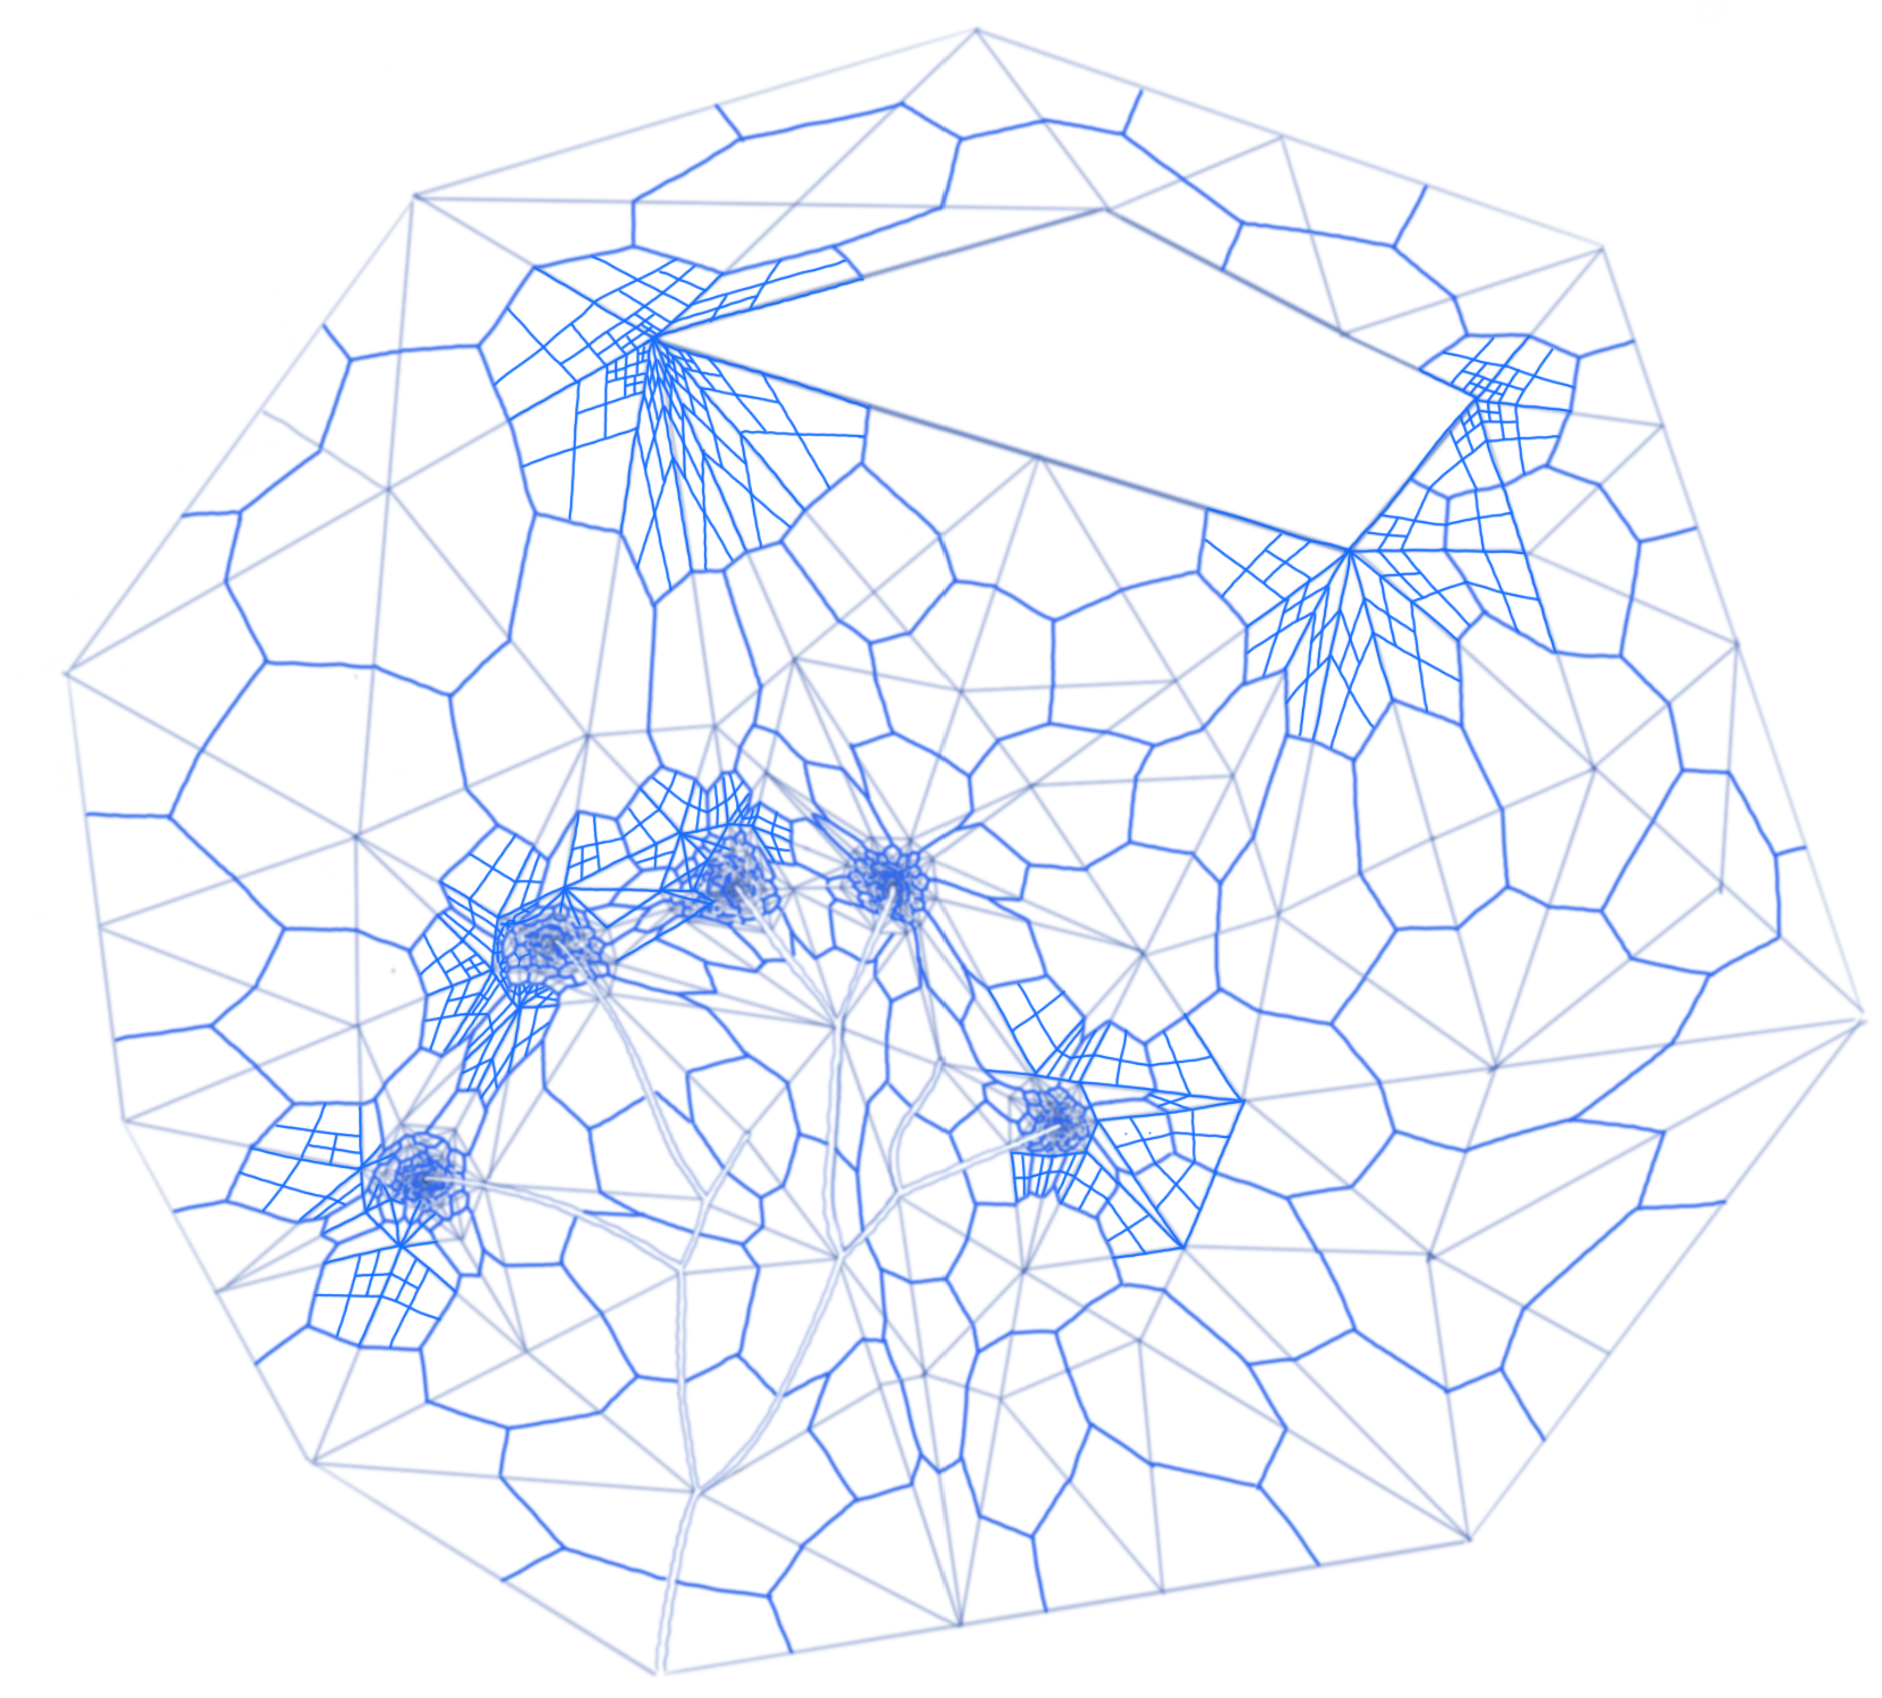
\includegraphics[width=0.9\textwidth]{figs/adaptive_refinment.png}        
          %Elementy siatki są dzielone w tych miejscach, gdzie błąd rozwiązania jest największy. W okolicy źródła pole zachowuje się jako $\frac{1}{\sqrt[2]{r}}$.
          \caption{Mesh elements are adapted in those places where the solution error is the greatest. Near the spring, the field behaves as $\sqrt{r}$.}
          \label{adaptive_refinment}
        \end{figure}

        %Istnieje wiele sposobów adaptacyjnego udoskonalania siatek. Podstawowa struktura algorytmu jest zawsze taka sama i składa się z pętli obejmującej następujące kroki:
        There are many ways to refine meshes adaptively. The basic structure of the algorithm is always the same and consists of a loop with the following steps:

        \begin{itemize}
          %\item Rozwiąż równanie różniczkowe cząstkowe na bieżącej siatce;
          %\item Oszacuj błąd w każdej komórce za pomocą pewnego kryterium wskazującego na błąd;
          %\item Zaznacz te komórki, które mają duże błędy do udoskonalania, zaznacz te, które mają szczególnie małe błędy do zgrubienia, a resztę zostawiamy;
          %\item Podziel lub połącz zaznaczone komórki, aby uzyskać nową siatkę;
          \item Solve a partial differential equation on the current mesh;
          \item Estimate the error in each cell with some error criterion;
          \item Select those cells that have large errors for refinement, mark those that have particularly small errors for bulging, and leave the rest;
          \item Split or combine selected cells to get a new grid.
        \end{itemize}

        %Poza tą strukturą istnieje jednak wiele sposobów osiągnięcia tego celu. Zasadniczo różnią się tym, jak dokładnie generuje się jedną siatkę z poprzedniej. Dla siatki z trójkątów, trójkąt zaznaczony do udoskonalenia jest dzielony na dwie części poprzez wprowadzenie jednej nowej krawędzi od środka najdłuższej krawędzi do przeciwległego wierzchołka. Oczywiście punkt środkowy od najdłuższej krawędzi musi być w jakiś sposób zrównoważony poprzez udoskonalenie komórki po drugiej stronie tej krawędzi (jeśli taka istnieje). Ta metoda nie działa w przypadku czworokątów, a przynajmniej nie jest łatwa. Powodem jest to, że elementy przejściowe utworzone z czworobocznych sąsiadów czworobocznej komórki, która ma zostać udoskonalona, byłyby trójkątami, a tego nie chcemy. W związku z tym podejście do adaptacyjności wybrane w Deal.II polega na wykorzystaniu siatek, w których sąsiednie komórki mogą różnić się poziomem udoskonalenia o jeden. Powoduje to, że węzły na interfejsach komórek należą do jednej strony, ale są niezrównoważone po drugiej. Powszechnym terminem dla nich są „wiszące węzły”. Jeśli udoskonalimy siatkę globalnie, błąd spadnie jako
        Outside of this structure, however, there are many ways to achieve this goal. They fundamentally differ in how accurately one mesh is generated from the previous one. For a triangular mesh, the triangle selected for refinement is split in two by inserting one new edge from the center of the longest edge to the opposite tip. Of course, the midpoint from the longest edge has to be balanced somehow by refining the cell on the other side of that edge (if any). This method does not work for quadrangles, at least it is not easy. The reason is that the transition elements created from the quadrilateral neighbors of the quadrilateral cell to be refined would be triangles, and we don not want that. Therefore, Deal.II approach to adaptability is to use grids where adjacent cells can differ in the level of refinement by one. This causes nodes on cell interfaces to belong to one side but are unbalanced on the other. The common term for these is "hanging nodes". If we refine the mesh globally, the error will behave as

        \begin{align*}
          \|\nabla(\phi-\phi_h)\|_{S} \le C h_\text{max}^p \| \nabla^{p+1} \phi \|_{S},
        \end{align*}

        %gdzie $C$ jest pewną stałą niezależną od $h$ i $\phi$, $p$ jest stopniem wielomianu używanego elementu skończonego, a $h_{max}$ jest średnicą największej komórki. Jeśli więc ważną jest największa komórka, to dlaczego mielibyśmy chcieć, aby siatka była drobna w niektórych częściach domeny, ale nie we wszystkich? Odpowiedź tkwi w spostrzeżeniu, że powyższy wzór nie jest optymalny. W rzeczywistości poniższe wzór jest lepszym oszacowaniem:
        where $C$ is some constant independent of $h$ and $\phi$, $\parallel \cdot \parallel_S $ is $\mathsf{L}_1-norm$, $p$ is the polynomial degree of the finite element used, and $h_{max}$ is the diameter of the largest cell. Above formula is not optimal, not only largest cells are important, but also value of solution derivative in some parts of domain also impacts error. Taking this into account, we can introduce better estimate:
        

        \begin{align*}
          \|\nabla(\phi-\phi_h)\|_{S}^2 \le C \sum_K h_K^{2p} \| \nabla^{p+1} \phi \|^2_K.
        \end{align*}

        %(Ponieważ $h_K\le h_\text{max}$, ta formuła natychmiast implikuje poprzednią, jeśli po prostu wyciągniesz rozmiar oczek z sumy.) Ta formuła sugeruje, że nie jest konieczne, aby największa komórka była mała, ale te komórki tak naprawdę potrzebują być małymi, gdzie $\| \nabla^{p+1} \phi \|_K$ jest duże! Innymi słowy: Siatka naprawdę musi być dokładna tylko wtedy, gdy rozwiązanie ma duże zmiany, na co wskazuje $p+1$ pochodna.
        (Since $h_K\le h_\text{max}$, this formula immediately implies the previous one if you simply take the mesh size from the sum.) This formula implies that it is sufficient that these cells need to be small where $\| \nabla^{p+1} \phi \|_K$ is big. In other words: The grid only really needs to be fine if the solution has large variations, as indicated by the $p+1$ derivative (Fig. \ref{adaptive_refinment}).
        
        %Oczywiście to oszacowanie a priori nie jest zbyt przydatne w praktyce, ponieważ nie znamy dokładnego rozwiązania $\phi$, a za tym idzie, że nie możemy obliczyć $\nabla^{p+1} \phi$. Ale możemy obliczyć numeryczne przybliżenia $\nabla^{p+1} \phi$ bazując tylko na dyskretnym rozwiązaniu $\phi_h$.
        In practice numerical aproximations are used to compute estimate of the $\nabla^{p+1} \phi$ derivative based on the discrete solution $\phi_h$.

      \paragraph{Riversim}
        
        %Powyższe rozumuwania teoretyczne są zaimplementowane w bibliotece Riversim w pliku `solver.hpp`:
        The above theoretical reasoning is implemented in the Riversim library in the file `solver.hpp`:
        
        \begin{mintedbox}{python}
          solver_params = SolverParams()
          solver_params.field_value = 1
          solver_params.quadrature_degree = 3
          solver_params.renumbering_type = 0
          solver_params.tollerance = 1e-12
          solver_params.num_of_iterrations =  6000
          solver_params.refinment_fraction = 0.1
          adaptive_refinment_steps = 1
        
          solver = Solver(solver_params)
          solver.openMesh(mesh)
          
          for j in range(adaptive_refinment_steps + 1):
              if j > 0:
                  solver.refineGrid()
              solver.setupSystem()
              solver.assembleSystem(boundary_conditions)
              solver.solve()\end{mintedbox}

    \section{Calculation of the $a_i$ coefficients}
      
      \begin{figure}[H]
        \centering
        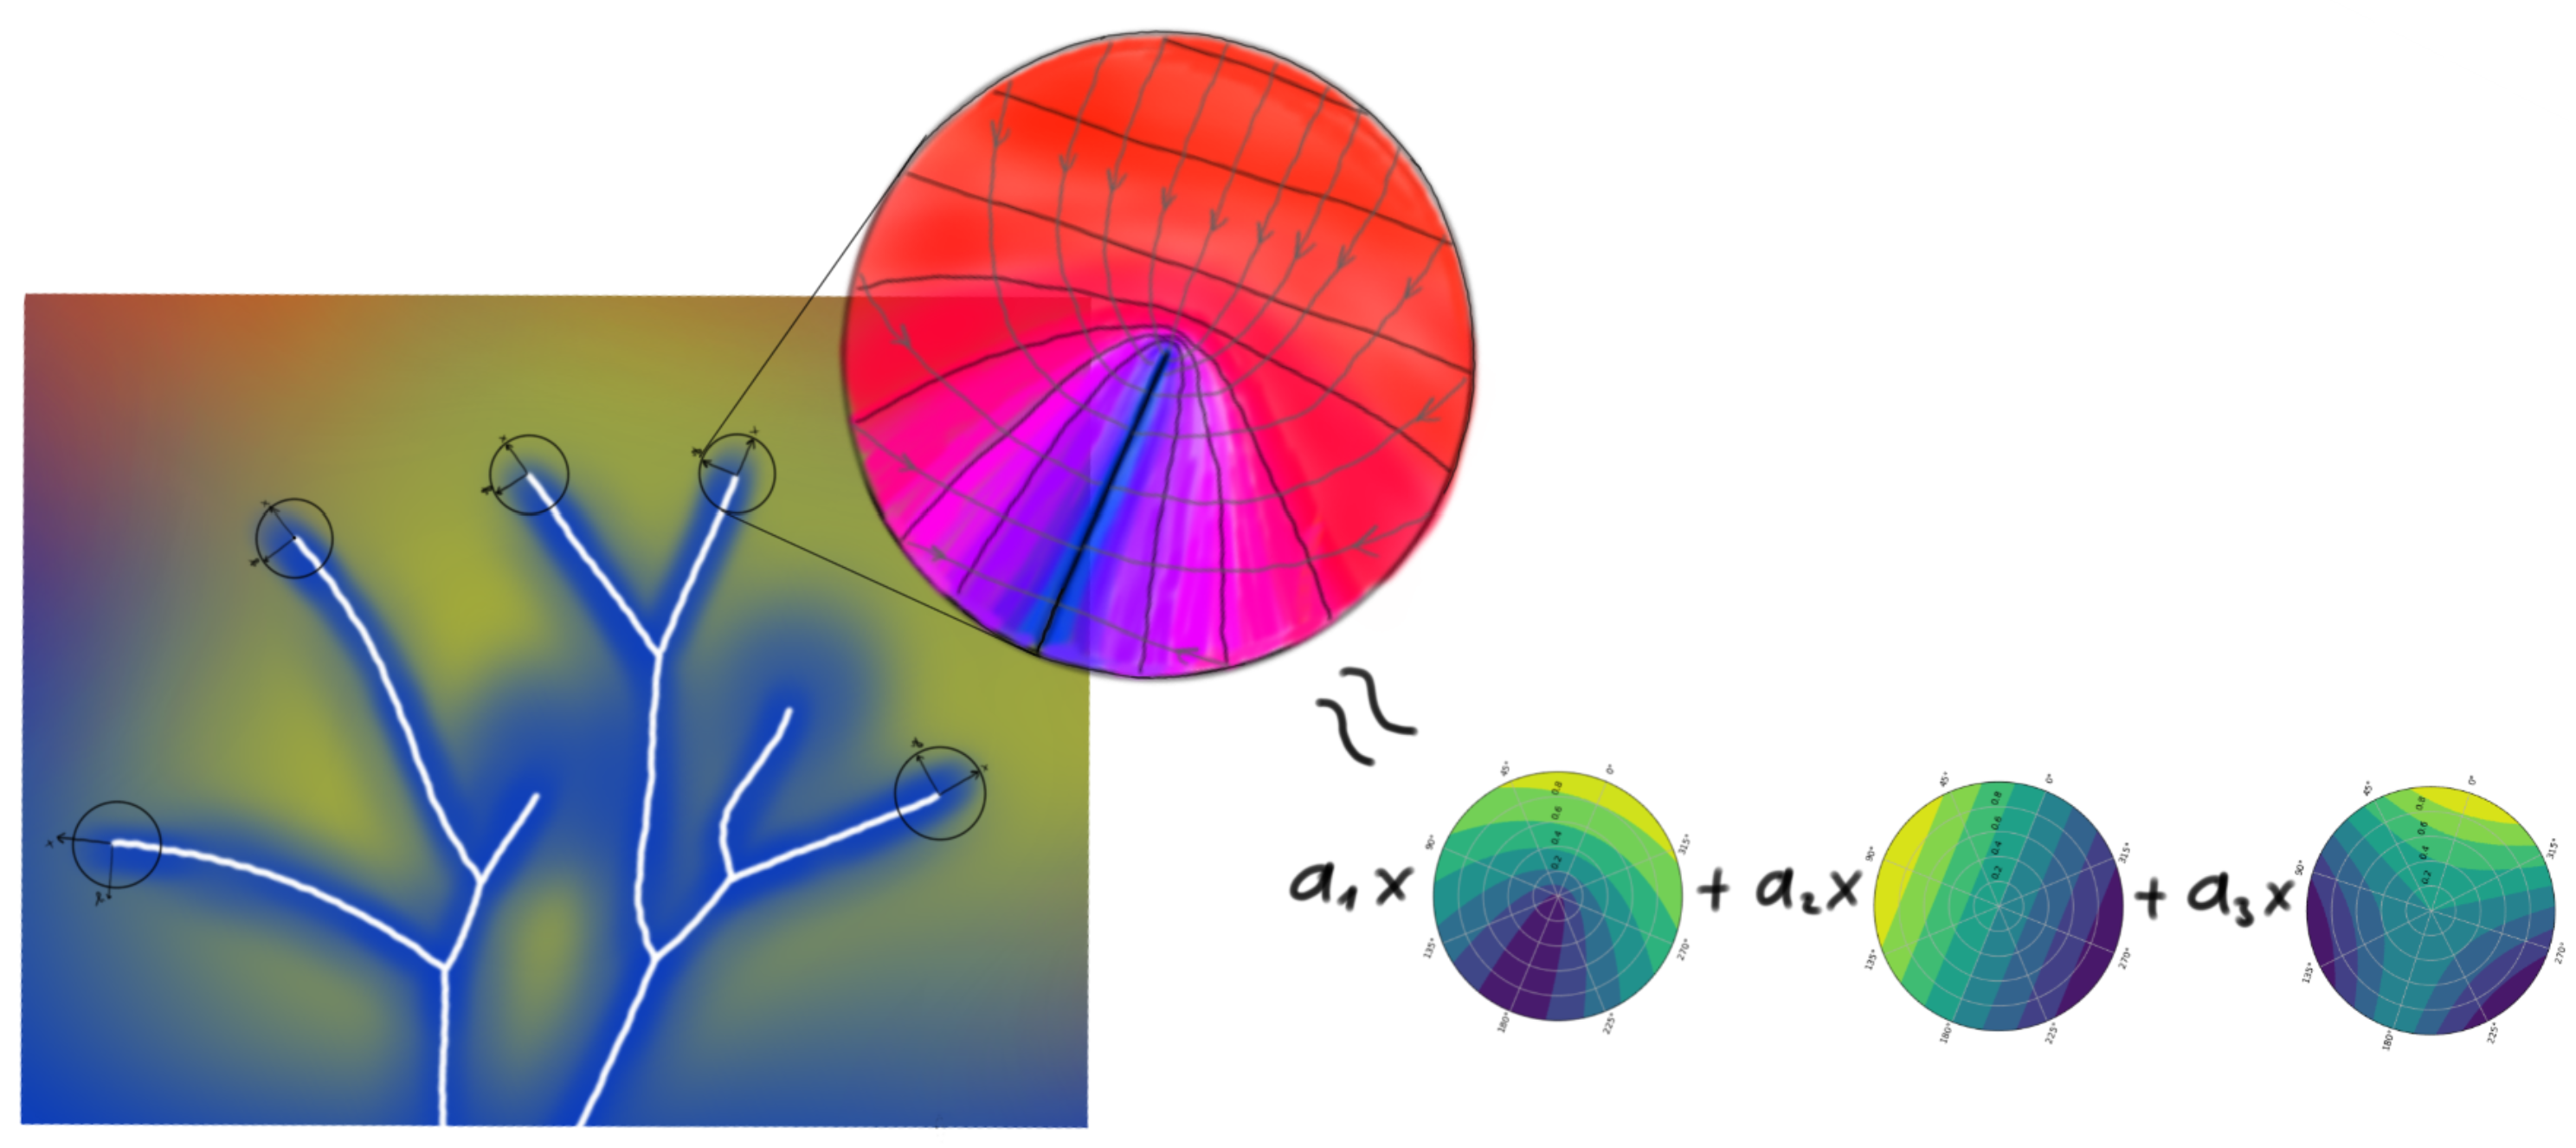
\includegraphics[width=0.9\textwidth]{figs/series_params_integration.png}        
        %Ilustracja rozkładu pola w okolicy źródła na współczynniki $a_n$.
        \caption{Illustration of the distribution of the field in the vicinity of the spring into $a_n$ coefficients.}
        \label{series_params_integration}
      \end{figure}

      %Powyżej już było pokazano że erozja jest największa w miejscach gdzie gradient pola jest największy. Takim miejscem z największym gradientem są oklicy źródeł. We współrzędnych biegunowych pole w pobliżu wierzchołka można rozszerzyć z pomocą równania \ref{series_params_integration}. Gdzie kazdy parameter $a_n$, $n \epsilon [1, 3]$ ma fizyczną interpretację (\ref{circle}, \ref{a3a1}) i jest powiązany z regułami wzrostu (\ref{velocity}). Współczynniki $a_n$ są wylicznę z postaci całkowej \ref{a1}, \ref{a2} i \ref{a3}. Aby zmniejszyć szum numeryczny uśredniamy postaci całkowe wzdłuż promienia $r$:
      It has already been postulated above that erosion is greatest in places where the field gradient is greatest. The areas in which the filed gradient is at its largest are usually located in the neighbourhood of the springs. In polar coordinates, the field near the spring can be expanded using equation (Fig. \ref{series_params_integration}). Each parameter $a_n$, $n \epsilon [1, 3]$ has a physical interpretation (\ref{circle}, \ref{a3a1}) and is associated with growth rules (\ref{velocity}). The coefficients $a_n$ are derived from the integral form (\ref{a1}, \ref{a2} and \ref{a3}). To reduce the numerical noise and to grasp field features(\ref{a3a1}) we average the integral forms along the radius $r$ to some $r_{max}$ value:
      
      \begin{equation}
        \label{a1_num}
        a_1 = \frac{\int^{r_{max}}_{0} \int^{\pi}_{-\pi} \phi(r, \theta) \cos \frac{\theta}{2} \omega(r) \textrm{d} \theta \textrm{d} r}{\int^{r_{max}}_{0} \int^{\pi}_{-\pi} \cos^2 \frac{\theta}{2} \omega(r) \textrm{d} \theta \textrm{d} r} \,,
      \end{equation} 
      
      \begin{equation}
        \label{a2_num}
        a_2 = \frac{\int^{r_{max}}_{0} \int^{\pi}_{-\pi} \phi(r, \theta) \sin \theta \omega(r) \textrm{d} \theta \textrm{d} r}{\int^{r_{max}}_{0} \int^{\pi}_{-\pi} \sin^2 \theta \omega(r) \textrm{d} \theta \textrm{d} r} \,,
      \end{equation}
      
      \begin{equation}
        \label{a3_num}
        a_3 = \frac{\int^{r_{max}}_{0} \int^{\pi}_{-\pi} \phi(r, \theta) \cos \frac{3 \theta}{2} \omega(r) \textrm{d} \theta \textrm{d} r}{\int^{r_{max}}_{0} \int^{\pi}_{-\pi} \cos^2 \frac{3 \theta}{2} \omega(r) \textrm{d} \theta \textrm{d} r}
      \end{equation}	

      %Gdzie $\omega(r)$ funkcja wagi ma postać:
      Where $\omega(r)$ the weight function is used to control field averaging:

      \begin{equation}
        \label{integration_weight}
        \omega(r) = \exp(-{(\frac{r}{r_{ref}})}^e)
      \end{equation}

      %Całka $\int^{r_{max}}_{r_{min}} \int^{\pi}_{-\pi} f(r, \theta) \textrm{d} \theta \textrm{d} r$ jak i równanie dla pola wód podziemnych, jest wyliczana numerycznie. Chociaż mamy dyskretnę rozwiązania pola wód podziemnych, ale wciąż otzrymanie wartości pola $\phi(x, y)$ w dowolnym punkcie nadal jest numerycznie skomplikowanym, o ile wymaga iterację po całej siatce regionu, a po znaleziniu odpowiedniego elementu -- interpolacje. Przez to przy aproksymówaniu całki skończoną sumą celem jest minimizacja ilości elementów. Kwadratura Gaussa jest dobrym rozwiązaniem, ale w danej pracy korzystamy z iteracujnej metody prostokątów:
      Integral $\int^{r_{max}}_{r_{min}} \int^{\pi}_{-\pi} f(r, \theta) \textrm{d} \theta \textrm{d} r$ is calculated numerically. Although we have a discrete groundwater field solution, still getting the value of the $\phi(x, y)$ field at any point is numerically complicated, as it requires iterating over the whole region mesh, and after finding the right element, evaluate value using quadrature. Thus, when approximating the integral with a finite sum, the goal is to minimize the number of elements. Gaussian quadrature is a good solution, but in this paper, we use the iterative method of rectangles:

      \begin{equation}
        \label{numerical_integral}
        \int^{b}_{a} f(x) \textrm{d} x = h \sum_{i = 0}^{n - 1} f(x_i + \alpha h),    \\
        h = \frac{a - b}{n}  
      \end{equation}

      %Ta całka jest rozwiązywana iteracyjnie aby osiągnąć potrzebną dokładność \cite{Press2007}:
      This integral is solved iteratively to achieve the necessary accuracy \cite{Press2007}:

      \begin{mintedbox}{c++}
        class Quadrature {
            public:
                size_t n = 0;
                virtual double next() = 0; };

        template<typename T> class Trapzd: virtual public Quadrature {
            public:
                T f;
                double s = 0., a, b;

                Trapzd(T func, double aa, double bb):
                    f{func}, a{aa}, b{bb} {}

                double next(){
                    ++n;
                    if (n==1) s = (b - a) / 2. * (f(a) + f(b));
                    else if (n > 1) {
                        auto tnm = pow(2., n - 2.), d = (b - a) / tnm, x = a + 0.5 * d, sum = 0.;
                        for(size_t j = 0; j < tnm; ++j) {
                            sum += f(x); x += d;
                        }
                        s = 0.5 * (s + d * sum);
                    }
                    return s;
                }
        }
        
        template<typename T> double qtrap(T func, double a, double b, double eps){
            auto s = 0., olds = 0.;
            auto t = Trapzd(func, a, b);
            for (size_t i = 0; i < (size_t)30; ++i) {
                s = t.next();
                auto cur_eps = abs(s - olds) / abs(olds);
                if (cur_eps < eps || (s < EPS && olds < EPS))
                    return s;
                olds = s;
            }
            throw Exception("qtrap: Too many steps in routine.");
        };\end{mintedbox}

        %W Riversimpy dla obliczenia współczynników $a_i$ służy metoda integrate (lub integrate\_new) klasy Solver:
        In Riversimpy, the integrate\_trap (or integrate\_new) method of the Solver class is used to calculate the $a_i$ coefficients:
        
        \begin{mintedbox}{python}
          integration_params = IntegrationParams()
          integration_params.eps = 1e-10
          integration_params.integration_radius = 3e-2
          integration_params.exponant = 2.0
          integration_params.weigth_func_radius = 1e-2        
          
          river_id = 1
          tip_point = rivers[river_id].tipPoint()
          tip_angle = rivers[river_id].tipAngle()

          ids_series_params = t_ids_series_params()
          ids_series_params[river_id] = solver.integrate_new(integration_params, tip_point, tip_angle)\end{mintedbox}

    \section{Growth and bifurcation rules, save and load from file, class Model}
      \begin{figure}[H]
        \centering
        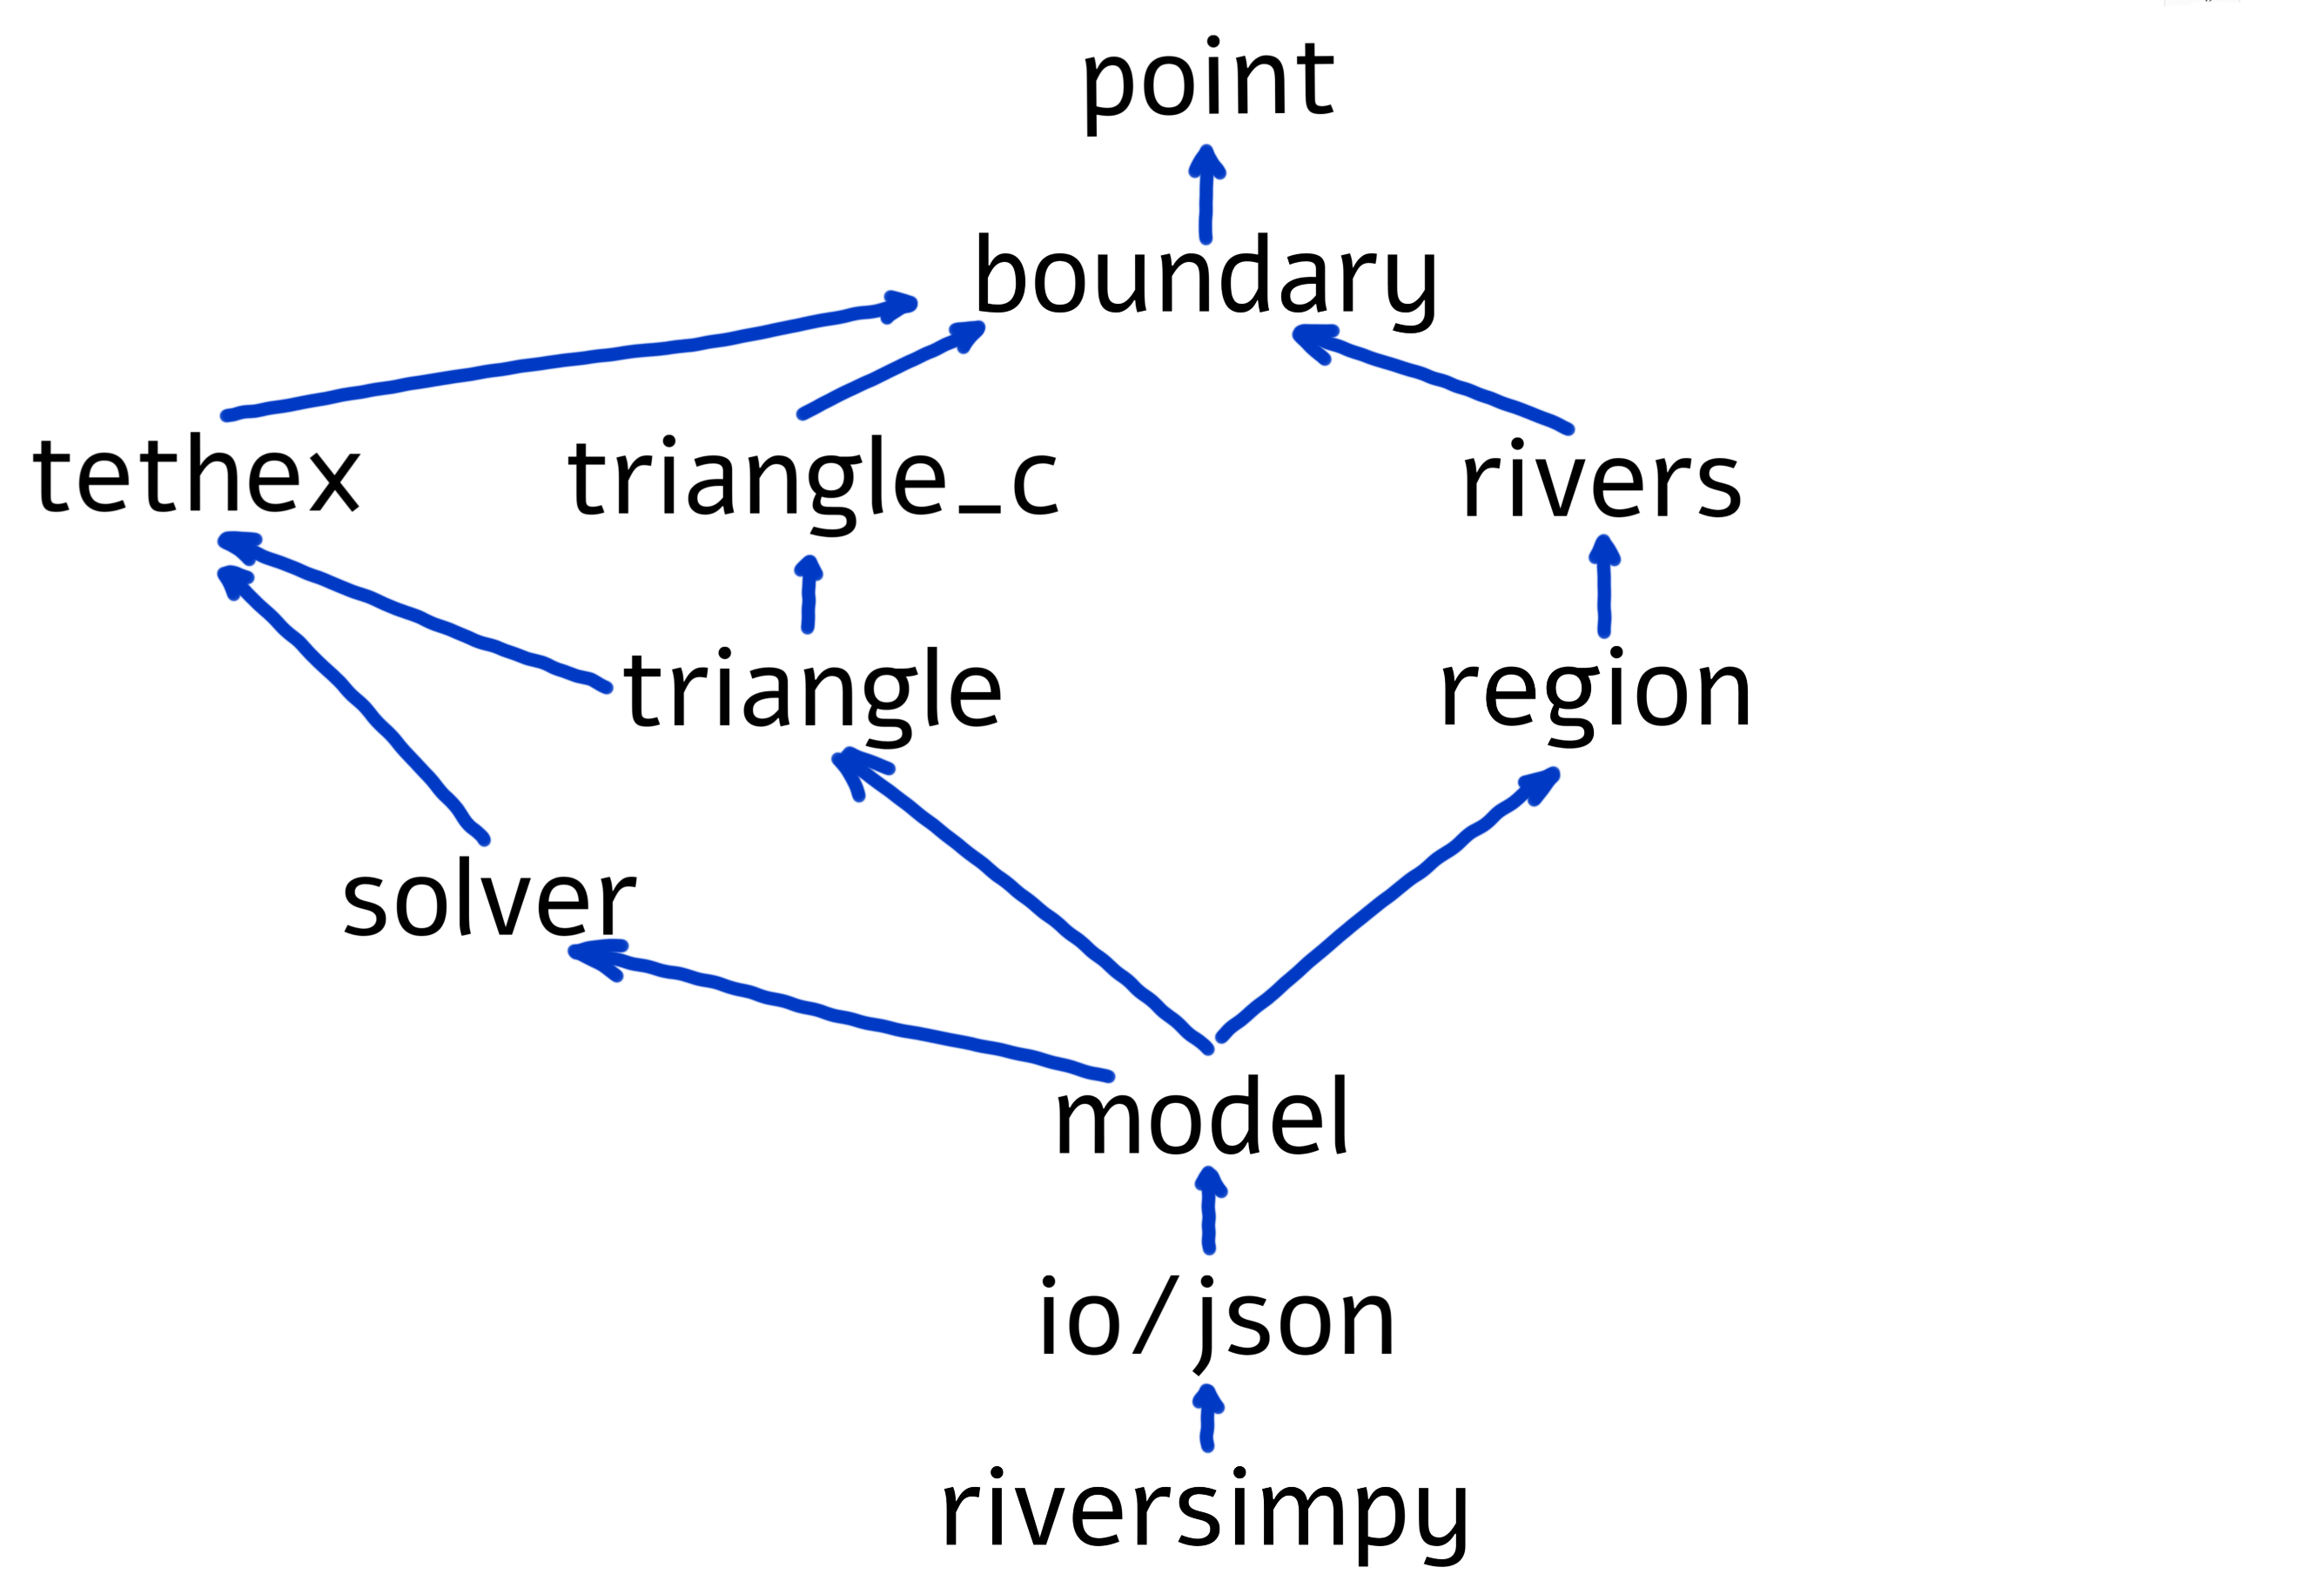
\includegraphics[width=0.5\textwidth]{figs/program_dependecy_graph.png}        
        %\caption{Graph zależności między modułami programu.}
        \caption{Graph of dependencies between program modules.}
        \label{program_strucutre}
      \end{figure}

    %Przedstawione powyżej klasy biblioteki Riversim już są wystarczają dla symulacji sieci rzecznych. Ale dla prostszego wykorzystania programu była stworzona klasa Model która zawiera wszystkie struktury danych programu, a tak że metody z regułami dla bifurkacji i wzrostu. Korzystajac z klasi Model możemy zapisać danę do pliku JSON, lub odczytać geometrie i wartości paratmetrów z pliku JSON:
    The Riversim library classes presented in Fig \ref{program_strucutre} are already sufficient to simulate river networks. But for simpler use of the program, the Model class was created which contains all the data structures of the program as well as methods with rules for bifurcation, growth and standard parameters. Using the Model class, we can save data to a JSON file, or read geometries and parameter values from a JSON file:

    \begin{mintedbox}{python}
      model = Model()
      model.initializeDirichlet();
      save(model, "river_initializet_to_dirichlet.json")
      
      model_dirichlet = Model()
      open(model_dirichlet, "river_initializet_to_dirichlet.json")\end{mintedbox}


  \chapter{Verification and validation}

    %Розв'язання росту мережі річки в полі Лапласа є складною задачею. Щоб отримати наближений розв'язок були використані методи дискретизації. Способи дискретизації включали в себе як і заміну гладких ліній мережі на дискретні із подальшим зменшення кількості точок дискретизації в залежності від кривизни. Дискретизація регіону на чотирикутні елементи і ступінь квадратури в кожному елементі. Кількість елементів суми для обчислення інтегралу параметрів довкола джерела. Але відомо що в границі із ростом дескритизації:
    Solving the growth of the river network in the Laplacian field is a difficult task. Several discretization methods were used to obtain an approximate solution: 
    
    \begin{itemize}
      \item Replacement of smooth network lines with discrete ones, followed by a reduction in the number of discretization points depending on the curvature;
      \item Discretization of the region into quadrilateral elements and the degree of quadrature in each element;
      \item The number of elements of the sum for calculating the integral of the parameters around the spring. But it is known that in the limit of high descritization;
      \item Split or combine selected cells to get a new grid.
    \end{itemize}
    
    In the limit of infinite discretization: 

    \begin{equation}
      \label{convergence}
      \lim_{n \to \infty} a_i(n)  = a_i
    \end{equation}

    %ми повинні отримати значення аналітичного розв'язку.
    where $n$ stands for total of each descritization, aproximate result should approach analytical solution value.
    
    \section{Convergence of integration and comparison with analytical result}

    \begin{figure}[H]
      \centering
      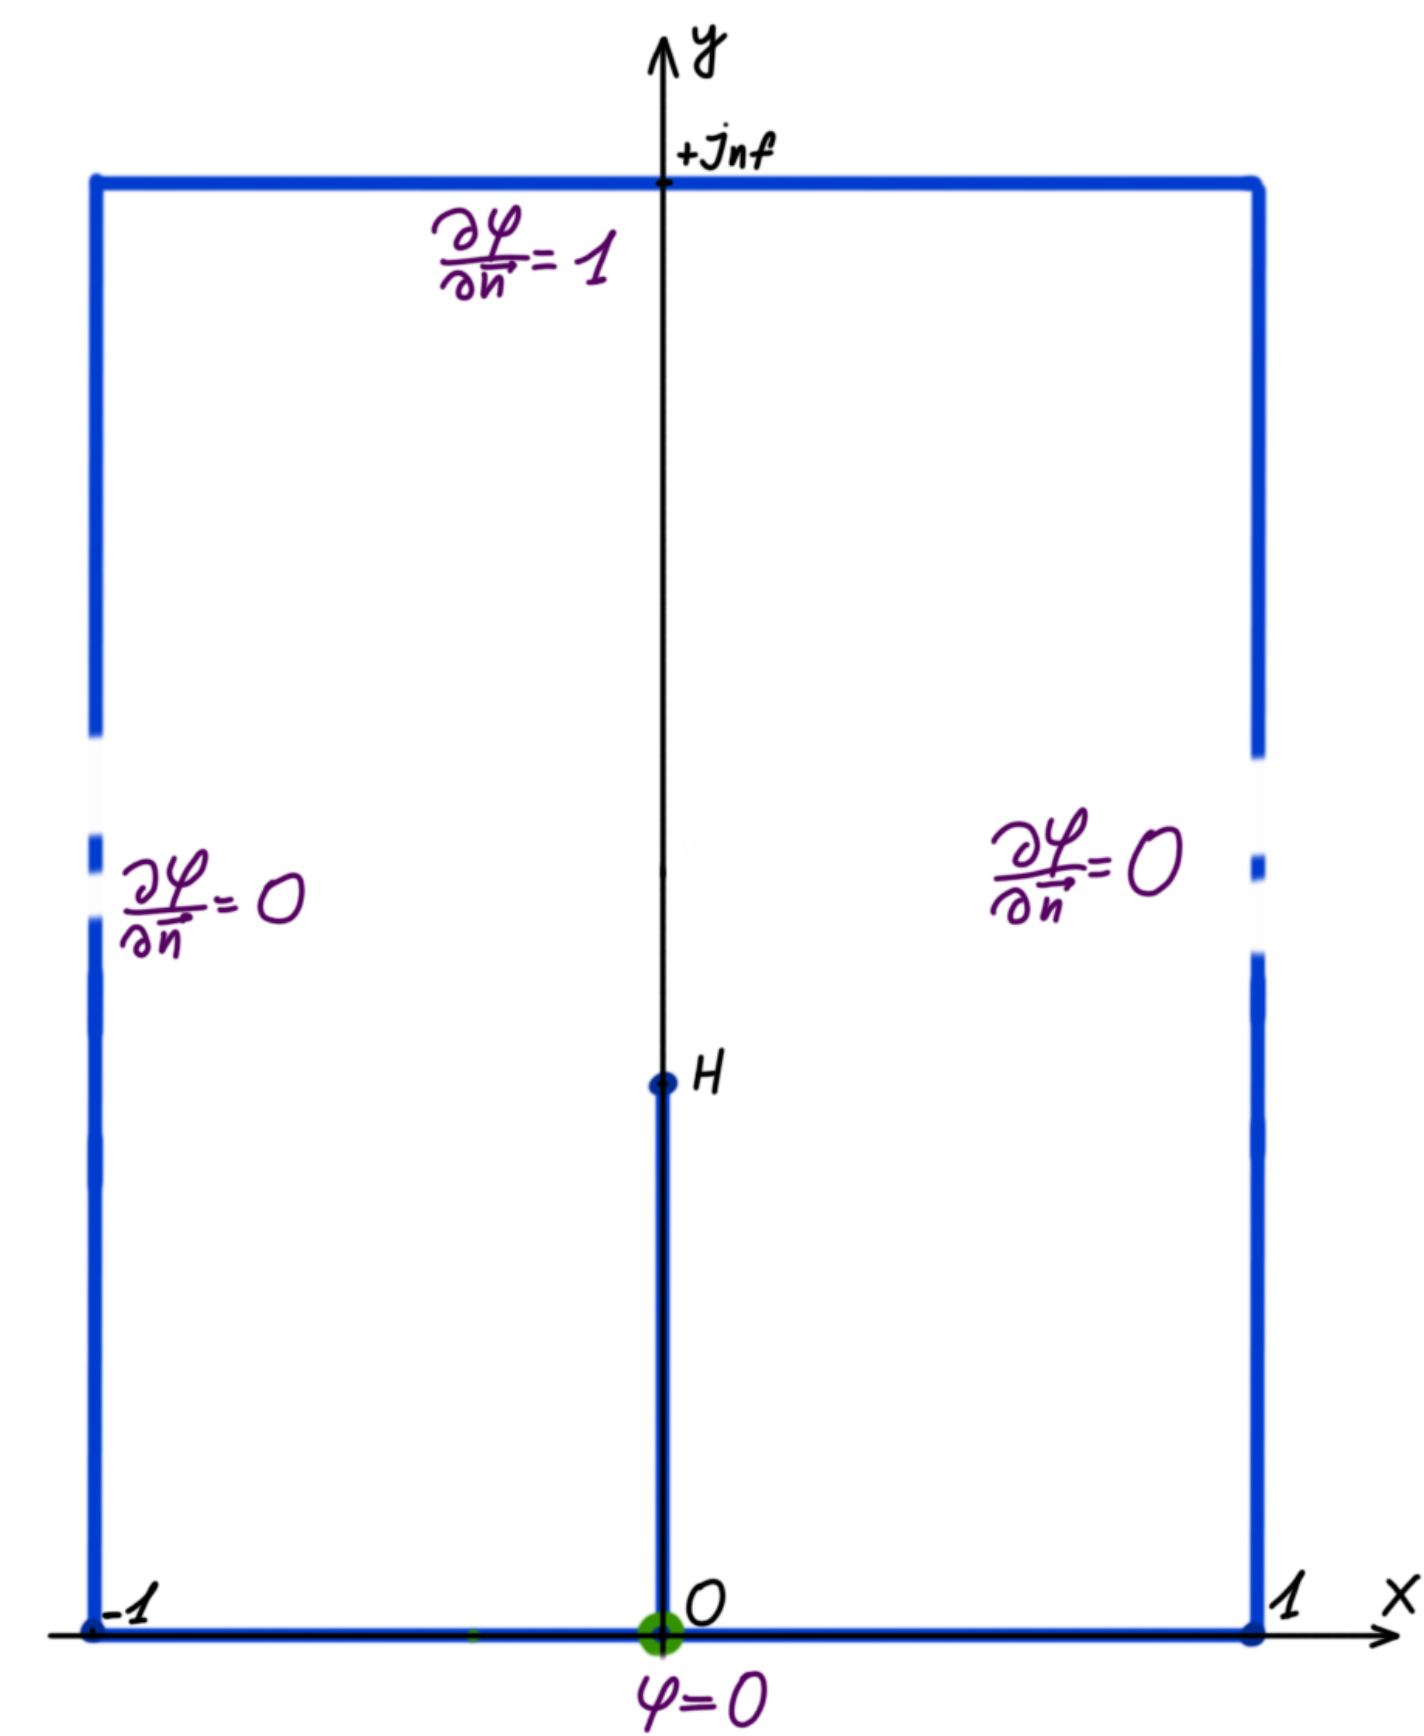
\includegraphics[width=0.5\textwidth]{figs/test_function_boundary.png}
      \caption{Semi-infinite domain with flux of the field coming from infinity used for evaluation of analitical value for $a_1$.}
      \label{test_boundary}
    \end{figure}

    %В роботі Ґубєц \cite{gubiec2008fingered} було отримано вираз для швидкості $\upsilon(H)$ взросту одної річки в наступних умовах: регіон прямокутної форми, висота котрого прямує до безмежності, ширина рівна $2$. На нижній грані звідки посередині звідки і зростає одна гілка річки маємо поглинаючі граничні умови ($\phi(0, y) = 0$), ізолюючі граничні умови на бокових гранях ($(\nabla \phi(x, y))_{\vec{n}} = 0$) і маємо сталий потік на безмежній відстані на верхній грані ($(\nabla \phi(x, y))_{\vec{n}} = 1$). 
    In the work of Gubiec et al.\cite{gubiec2008fingered}, an expression was obtained for the rate $\upsilon(H)$ of the growth of one river under the following conditions: a rectangular region with infinite height, the width is $2$. In the middle of lower face, river branch with lenght $H$ is set (Fig. \ref{test_boundary}). At the bottom face and river branch, absorbing boundary conditions ($\phi(0, y) = 0$) are set, insulating boundary conditions on the side faces ($(\nabla \phi(x, y))_{ \vec{n}} = 0$) and constant flow at an infinite distance on the upper face ($(\nabla \phi(x, y))_{\vec{n}} = 1$).

    \begin{equation}
      \label{velocity_analytical}
      \upsilon(H) = \sqrt{\frac{2}{\frac{\pi}{2}\coth(\frac{\pi}{2}H)}} \,.
    \end{equation}
    
    %В нашому випадку ми не можемо задати безмежну відстань верхньої грані, тому ми обмежимося достатньо витягнутим прямокутником ($50/2$).
    In our case, semi-infinite domain is aproximated by elongated rectangle (height -- $50$, width --$2$).

    \begin{figure}[H]
      \centering
      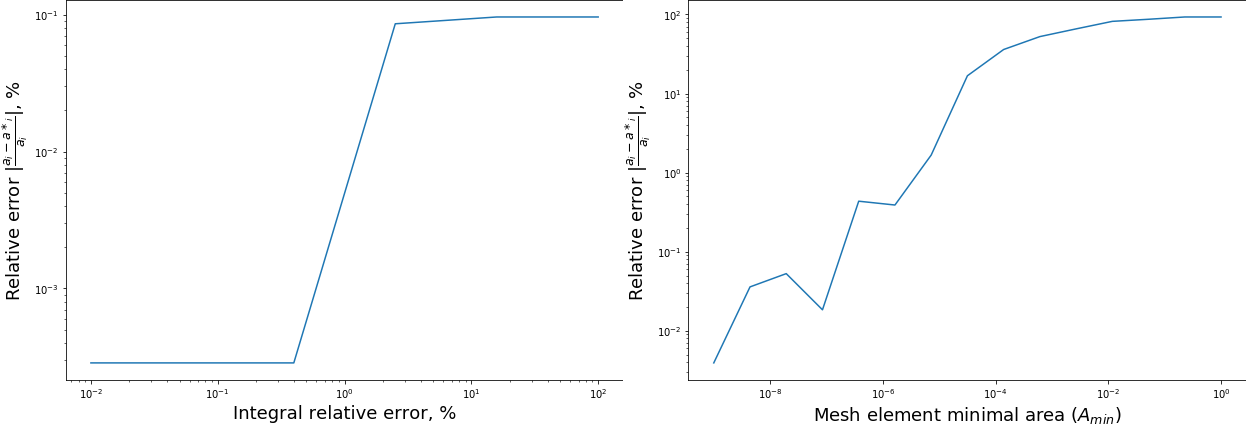
\includegraphics[width=1\textwidth]{figs/convergence.png}        
      \caption{Left plot shows how the relative error in percentage between evaluated and analitical value $a_1$ is converging. Right plot shows convergence when number of mesh elements are increased.}
      \label{convergence_new}
    \end{figure}

  \chapter{Summary}

    %В цій праці магістерській ми розглянули розвиток просторової мережі на прикладі еволюції мережі річок. Спочатку ми зарепрезентували теоретичну модель з фокусом на підземні води і ерозію в околиці джерел. Запровадили спрощення одновимірної річки. Показали як описати поле підземних вод $\phi(x, y)$ в околиці джерела за допомогою пареметрів розкладу $a_i$. Тоді показали як параметри $a_i$ можна інтерпретувати і як вони пов'язані із динамікою розвитку мережі.\par
    In this master's thesis, we considered the development of the spatial network using the example of the evolution of the river network. First, we represented a theoretical model with a focus on groundwater and erosion in the vicinity of springs. Simplification of the one-dimensional river was introduced. It was shown how to describe the field of groundwater $\phi(x, y)$ in the vicinity of the spring using the $a_i$ parameters. Then it was shown how the parameters $a_i$ can be interpreted and how they are related to the dynamics of the network development.\par

    %Далі ми запропонували своє чисельне рішення цієї складної проблеми взаємозалежності мережі і поля під впливом якого, вона розвивається у бібліотеці Python -- Riversim. Детально описали структуру бібліотеки із прикладами її використання. Як задавати довільну початкову геометрію. Як задати початкову позицію джерел із яких буде відбуватися розвиток річки. В якій структурі даних зберігається мережа річки і як із нею працювати. Як задавати граничні умови і яких видів вони присутні у програмі. Те, як із початкової геометрії згенерувати сітку з допомогою Tethex i Triangle С++ бібліотек. Після цього як отримати поле підземних вод з допомогою методу FEM, який імплементований в бібліотеці Deal.II. Як обчислити параметри  $a_i$ використовуючи чисельний інтеграл.\par
    Next, we described our open source numerical solution to the river network development in the Python library -- Riversim. The structure of the library was described in detail with examples of its use: 
    
    \begin{itemize}
      \item Setting arbitrary initial geometry;
      \item Setting initial position of the springs;
      \item How to work with Rivers class, which holds river network related data;
      \item Setting of boundary conditions;
      \item Mesh generation, using capabilities based on Triangle and Tethex C++ libraries;
      \item Groundwater field evaluation using the FEM method, which is implemented in the Deal.II C++ library;
      \item Evaluation of $a_i$ parameters using a numerical integral.
    \end{itemize}

    %Коротко показана верифікація бібліотеки Riversim, приклад програми для обрахування розвитку мережі і деякі резултати симуляцій.\par
    The verification of the Riversim library, an example of a program for calculating the development of the network, simulations result in Laplacian and Poisson field for different $\eta$ are shown.\par

    \section*{Acknowledgements}
      
      I would like to thank Olivier Devauchelle from Institut de Physique du Globe, Paris and Hansjörg Seybold from ETH Zurich for sharing the code of river network growth simulation in FreeFEM++ which helped me to came out with my own solution. And also thanks to Stasiek Żukowski for using Riversim software for backward simulation and giving me usage experience of the program.

    \bibliographystyle{unsrt_initials} %ieeetr
    \bibliography{bibliography}

  \appendix

  \chapter{The main loop of the program}
    
    %Instalacja biblioteki Riversim w Python3 (tylko Linux):
    Installing the Riversim library in Python3 (Linux only):
    
    \begin{mintedbox}{bash} 
      python3 -m pip install riversim\end{mintedbox}
    
    %Skrypt Python symulujący rozwój sieci rzecznej napisany w oparciu biblioteki riversm:
    Python script simulating the development of the river network written on the basis of the Riversim library:

    \begin{mintedbox}{python} 
      from riversim import *
      import numpy as np

      m = Model()
      m.InitializeDirichlet()

      solver = Solver(m.solver_params)
      triangle = Triangle(m.mesh_params)
      mesh = TethexMesh()

      dynamic_river_ids = m.rivers.tipBranchesIds()

      for i in range(m.number_of_steps):
          m.boundary = BoundaryGenerator(\
              m.sources, \
              m.region, \
              m.rivers, \
              m.region_params)

          num_of_intersects = NumOfBoundaryIntersection(m.boundary, m.rivers.tipBoundary())
          if num_of_intersects > 0:
              break

          empt_rivers = Rivers()
          empt_source = Sources()
          only_boundary = BoundaryGenerator(empt_source, m.region, empt_rivers, m.region_params)
          distance_to_boundary = DistanceFromPointsToBoundary(only_boundary, m.rivers.tipPoints())
          if distance_to_boundary <= m.integr_params.integration_radius:
              break

          if len(m.boundary.vertices) == 0:
              break 

          # mesh will be refined aroud growing tip points
          tip_points = t_PointList()
          for id in dynamic_river_ids:
              tip_points.append(m.rivers[id].tipPoint())
          triangle.mesh_params.tip_points = tip_points
          mesh = triangle.generate(m.boundary, m.region.holes)
              
          solver.openMesh(mesh)
          for j in range(m.solver_params.adaptive_refinment_steps + 1):
              if j > 0:
                  solver.refineGrid()
              solver.setupSystem()
              solver.assembleSystem(m.boundary_conditions)
              solver.solve()

          id_series_params = t_ids_series_params()
          max_a1 = 0
          for id in dynamic_river_ids:
              tip_point = m.rivers[id].tipPoint()
              tip_angle = m.rivers[id].tipAngle()
              id_series_params[id] = solver.integrate_new(m.integr_params, tip_point, tip_angle)
              if id_series_params[id][0] > max_a1:
                  max_a1 = id_series_params[id][0]

          for id_series_param in id_series_params:
              id = id_series_param.key()
              series_param = id_series_param.data()
              if m.qGrowth(series_param):
                  l = m.rivers[id].lenght()
                  if m.qBifurcate(series_param, l):
                      tip_point = m.rivers[id].tipPoint()
                      tip_angle = m.rivers[id].tipAngle()
                      br_left = Branch(tip_point, tip_angle + m.bifurcation_angle)
                      br_left.addPoint(Polar(m.ds, 0), m.region_params.river_boundary_id)
                      br_right = Branch(tip_point, tip_angle - m.bifurcation_angle)
                      br_right.addPoint(Polar(m.ds, 0), m.region_params.river_boundary_id)
                      ids = m.rivers.addSubBranches(id, br_left, br_right)

                      # add new branches
                      dynamic_river_ids.append(ids.left)
                      dynamic_river_ids.append(ids.right)

                      # and remove parent from growth evaluation
                      for f in range(len(dynamic_river_ids)):
                          if dynamic_river_ids[f] == id:
                              del dynamic_river_ids[f]
                              break
                  else: 
                      m.rivers[id].addPoint(\
                          m.nextPoint(series_param, l, max_a1),\
                          m.region_params.river_boundary_id)
              else:
                  # remove river from growth evaluation
                  for f in range(len(dynamic_river_ids)):
                      if dynamic_river_ids[f] == id:
                          del dynamic_river_ids[f]
                          break

          if debug:
              save(m, "debug " + str(i) + ".json")

          if not dynamic_river_ids:
              break
      \end{mintedbox}

      \section{Examples of networks}
        
        \begin{figure}[H]
          \centering
          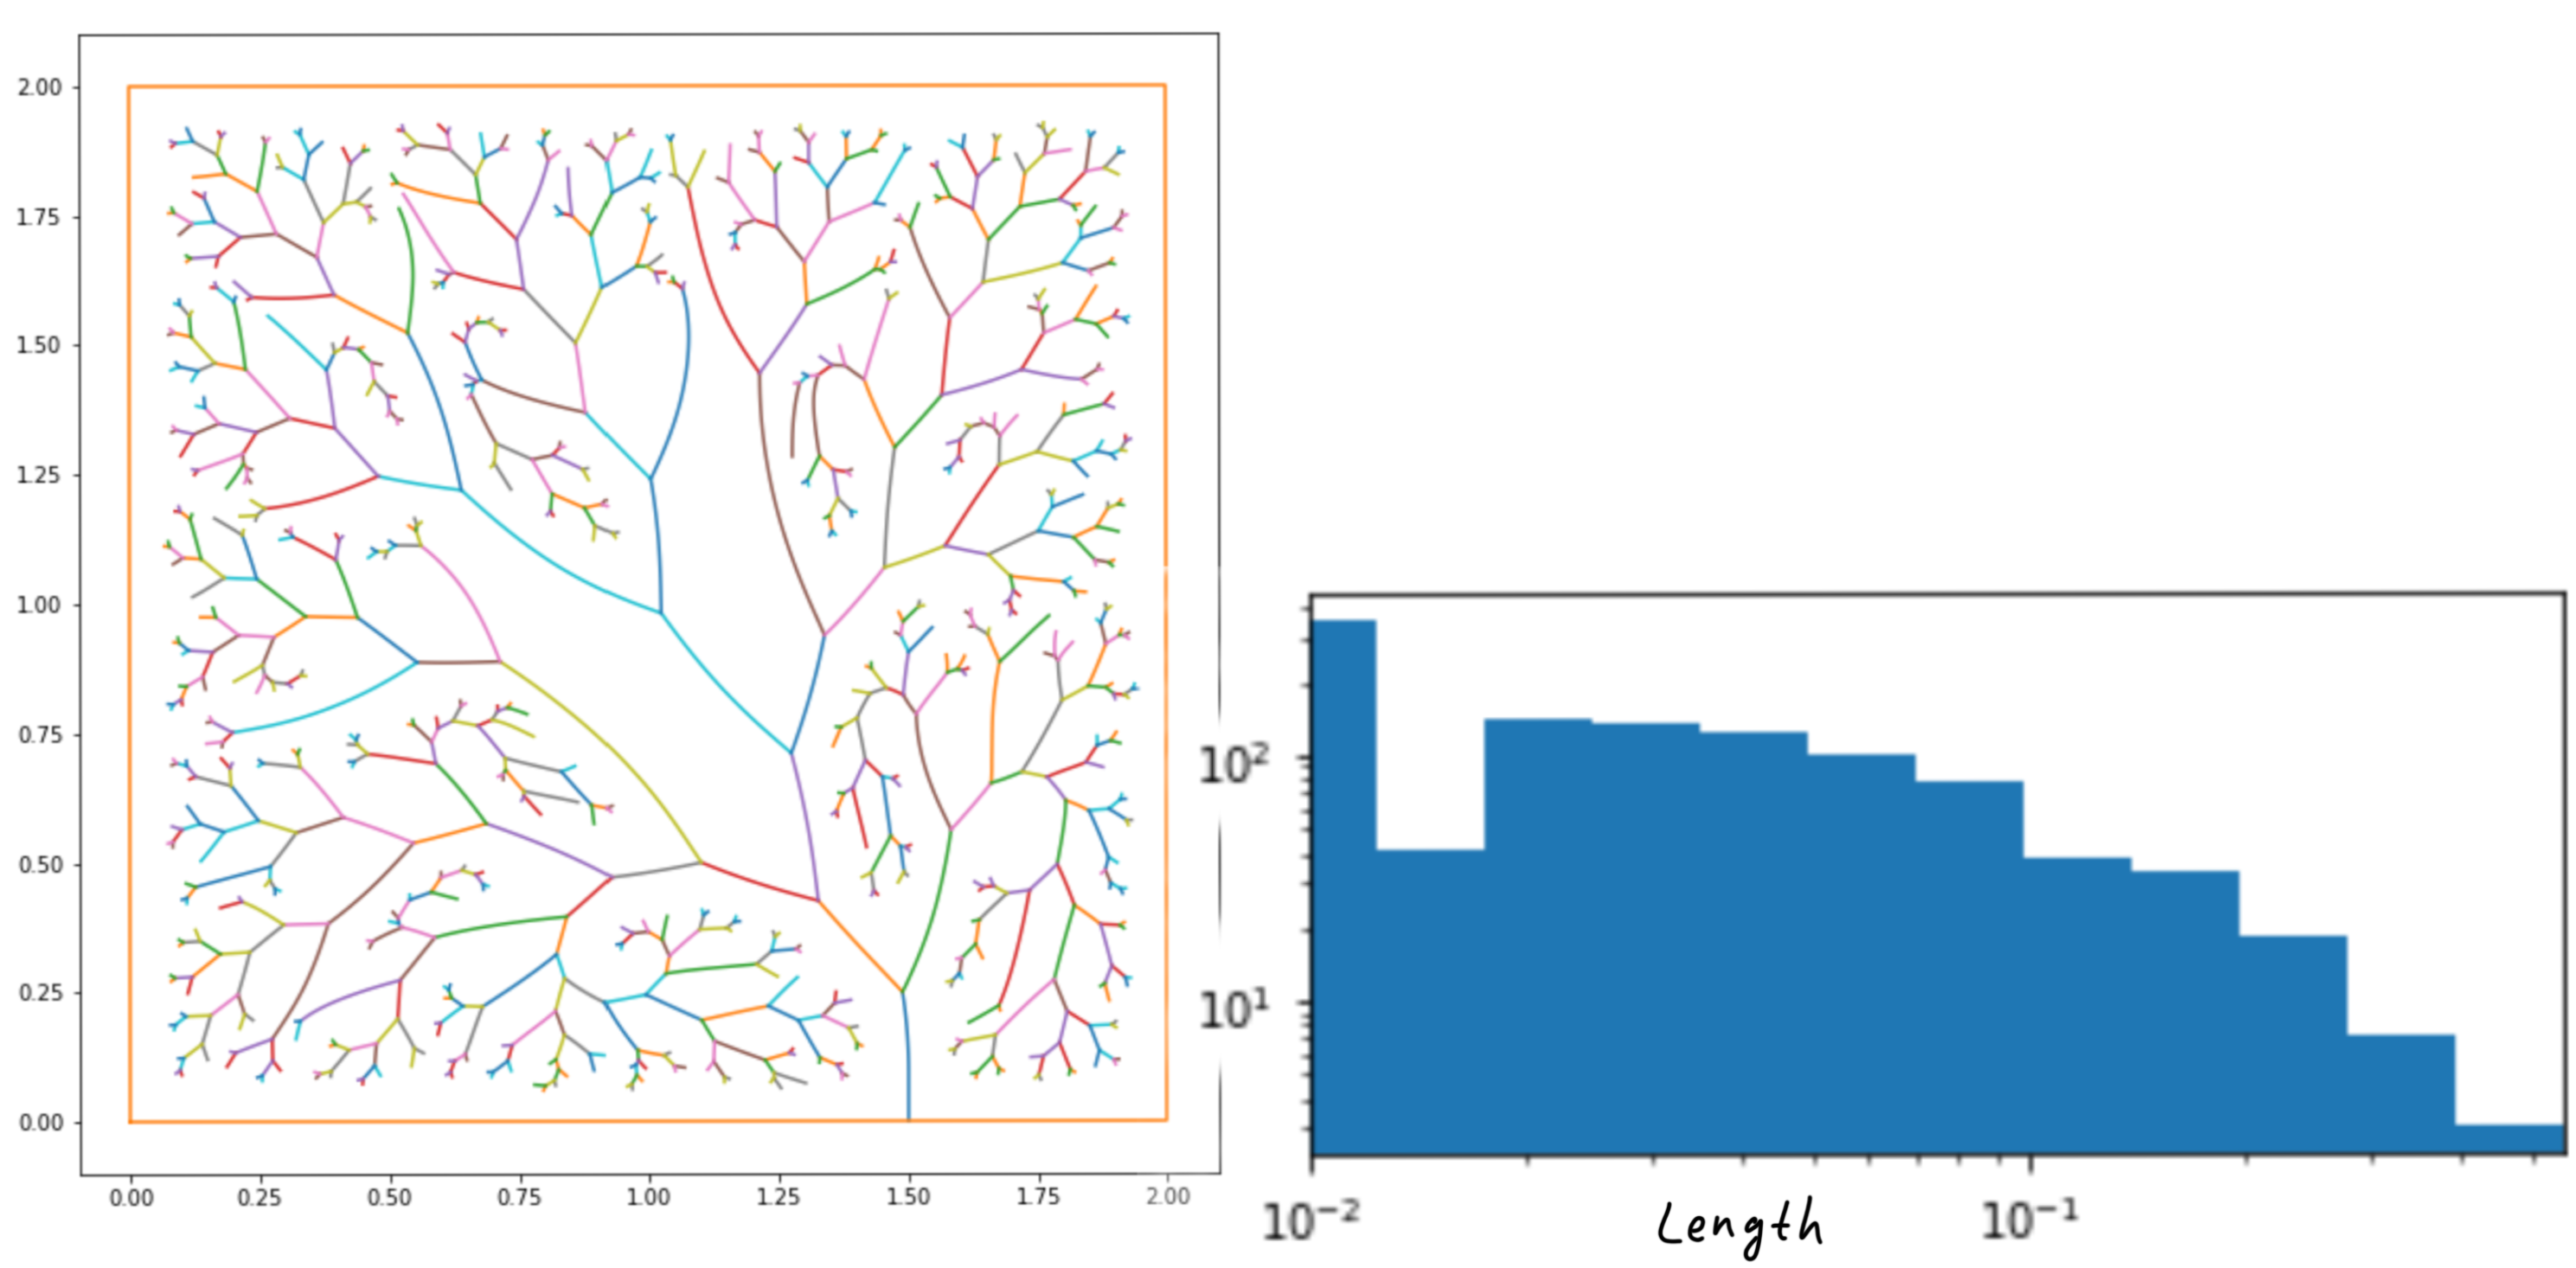
\includegraphics[width=1\textwidth]{figs/histogram.png}        
          \caption{Left plot shows river network grown in Poisson field. Right plot shows length histogram of each line from which river network consists. You can see peak at $Length = 0.01$, it is due to numerical parameter which limits minimal river length between biffurcation points and in this simulation it is equal to $0.01$.}
        \end{figure}

        \begin{figure}[H]
          \centering
          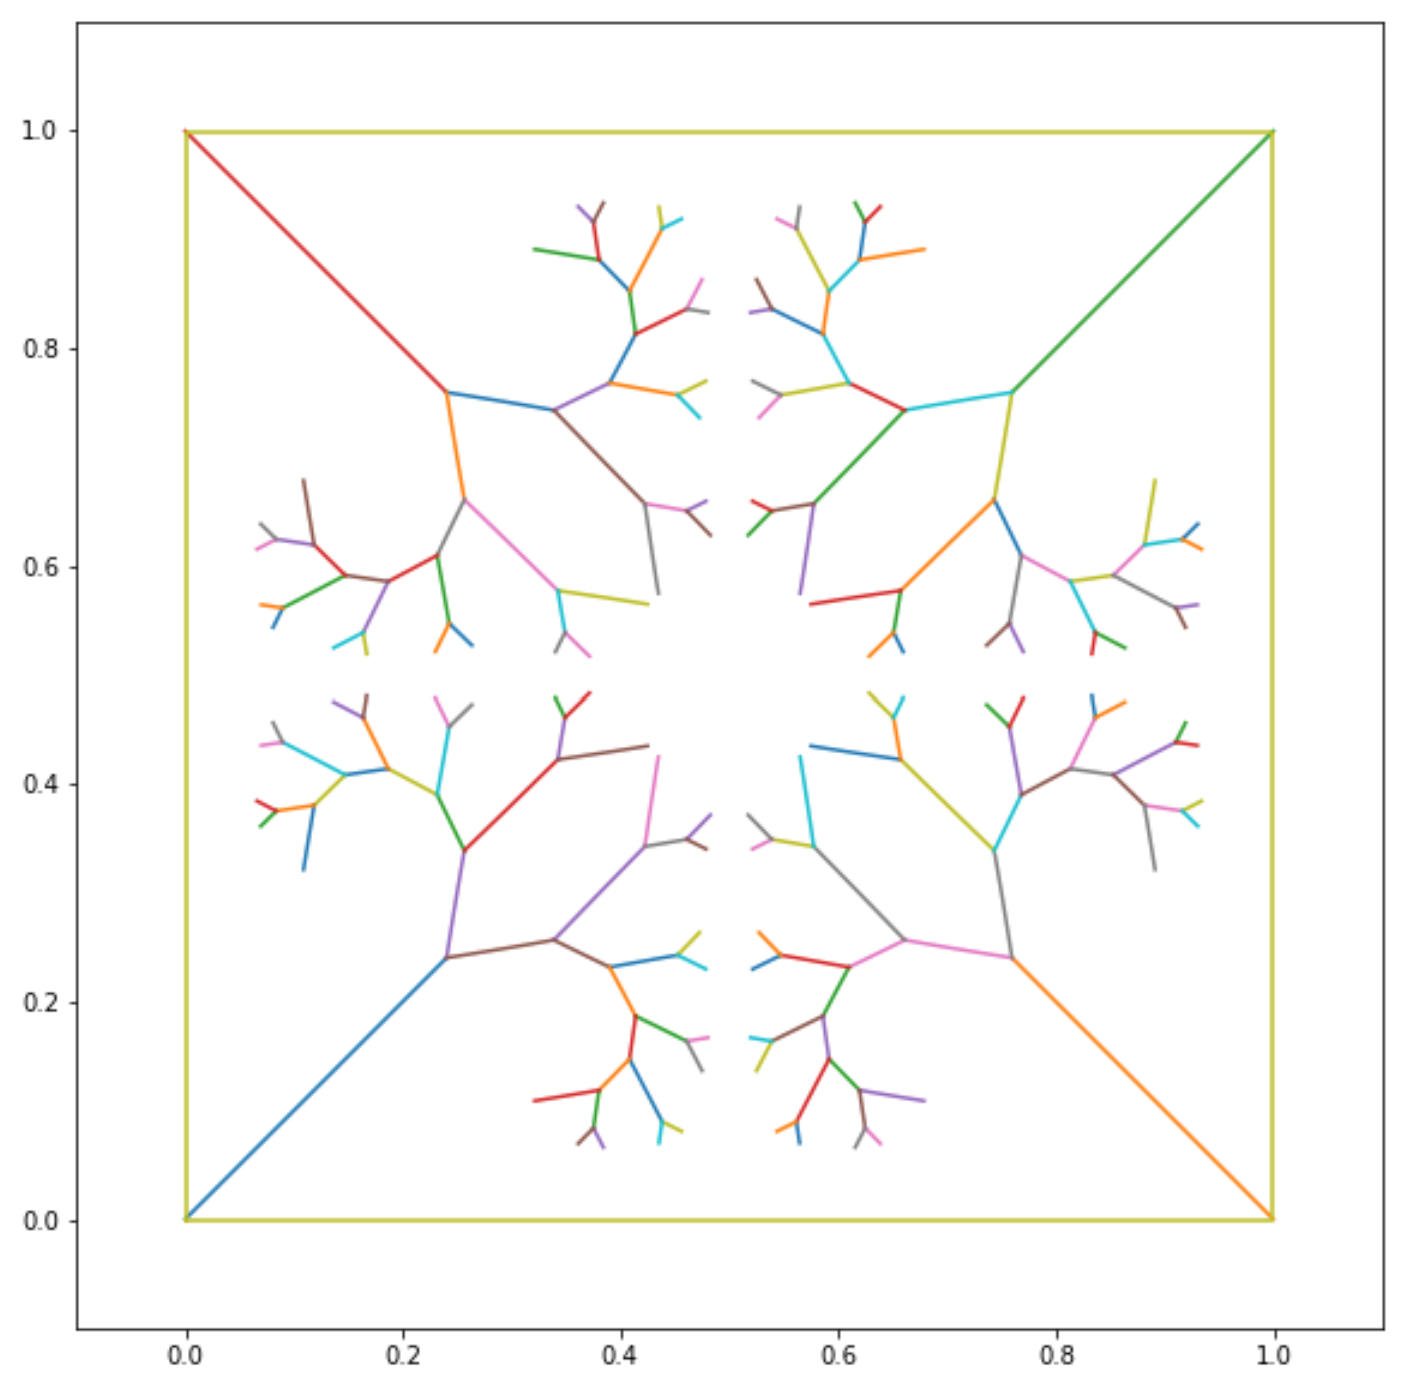
\includegraphics[width=1\textwidth]{figs/symmetic_rivers.png}        
          \caption{Initial region of this simulaiton is rectangle where each corner is the spring of the river. After growth of the each river network in Poisson field, you can see that figure is still symmetric.}
        \end{figure}

\end{document}